% **********************************************************
%                                                          *
% Marko Lalovic                                            *
% Partial Drawings of Complete Graphs                      *
% Wed Mar 12 18:42:04 CEST 2014                            *
%                                                          *
% **********************************************************
\documentclass[oneside, 12pt]{book}


% **********************************************************
%    Packages
% **********************************************************
\usepackage[utf8]{inputenc}
\usepackage[english]{babel}
\usepackage[pdftex]{graphicx}
\usepackage[pdftex,
            colorlinks=true,
            citecolor=black, filecolor=black,
            linkcolor=blue, urlcolor=black,
            pagebackref=false,
            pdfproducer={LaTeX},
            pdfcreator={LaTeX},
            hidelinks]{hyperref}
\usepackage{fancyhdr}
\usepackage{afterpage}
\usepackage{amsmath}
\usepackage{amssymb}
\usepackage{amsthm}
\usepackage{url}
\usepackage{listings}
\usepackage{enumitem}
\usepackage{verbatim}
\usepackage{parskip}
\usepackage[hidelinks]{hyperref}
\usepackage{tcolorbox}
\usepackage{pdfpages}
\usepackage{anyfontsize}
\usepackage{linguex}
\usepackage{mathtools}
\usepackage{float}
\usepackage{booktabs}
\usepackage{times}

% additional packages
\usepackage{bbm}
\usepackage{support-caption}
\usepackage{subcaption}
\usepackage{accents} % for underaccent in undersym notation
% \usepackage{breqn} % it breaks binom
\usepackage{microtype}

%tikz
\usepackage{a4}
\usepackage{tikz}
\usetikzlibrary{positioning}
\usetikzlibrary{arrows}
\usetikzlibrary{calc}
%\usetikzlibrary{matrix}
%\usetikzlibrary{shapes}
%\usetikzlibrary{decorations.markings}
%\usetikzlibrary{decorations}
\usepackage{tkz-euclide}
\usepackage{yfonts}


% **********************************************************
%    Commands and Settings
% **********************************************************
\microtypecontext{spacing=nonfrench}
\captionsetup[table]{position=bottom}

\newcommand*{\quedb}{\hfill\ensuremath{\square}}%
\setlength{\headheight}{15pt} % headheight too small
\renewcommand{\baselinestretch}{1.3} % line spacing
\renewcommand{\chaptermark}[1]%
{\markboth{\MakeUppercase{\thechapter.\ #1}}{}} \renewcommand{\sectionmark}[1]%
{\markright{\MakeUppercase{\thesection.\ #1}}} \renewcommand{\headrulewidth}{0.5pt}
\renewcommand{\footrulewidth}{0pt}

\pagestyle{fancy}
\fancyhf{}

% headers upper case
\fancyhead[L,RO]{\thepage} \fancyhead[LO]{\rightmark} \fancyhead[R]{\leftmark}
\newcommand{\autfont}{\Large}
\newcommand{\titfont}{\LARGE\bf}
\newcommand{\clearemptydoublepage}{\newpage{\pagestyle{empty}\cleardoublepage}}
\setcounter{tocdepth}{1}
\newcommand{\qedwhite}{\hfill \ensuremath{\Box}}

\definecolor{blue}{RGB}{51,105,232}
\definecolor{yellow}{RGB}{238,118,0}
\definecolor{orange}{RGB}{213,15,37}
\definecolor{red}{RGB}{139,37,0}
\definecolor{grey}{RGB}{211,211,211} 
\definecolor{gray}{RGB}{211,211,211} 
\definecolor{green}{RGB}{0,153,37}
\definecolor{color-trapezoid}{RGB}{211,211,211} 
\definecolor{color-inside}{RGB}{211,211,211} 
\definecolor{color-parallelogram}{RGB}{211,211,211} 
\definecolor{color-CL}{RGB}{211,211,211}

\theoremstyle{plain}
\newtheorem{theorem}{Theorem}
\newtheorem{lemma}[theorem]{Lemma}
\newtheorem{proposition}[theorem]{Proposition}
\newtheorem{corollary}[theorem]{Corollary}
\newtheorem{definition}[theorem]{Definition}
\newtheorem{properties}[theorem]{Properties}

\newcommand{\norm}[1]{\left\lVert#1\right\rVert}
\providecommand{\keywords}[1]{\textbf{\textit{Keywords:}} #1}

% geometry macros
\newcommand{\quadsym}{\Diamond}
\newcommand{\rectansym}{\Box}
\newcommand{\trisym}{\triangle}
\newcommand{\abovesym}[1]{\tilde{#1}}
\newcommand{\undersym}[1]{\underaccent{\tilde}{#1}}

% three-rule function
\newcommand{\threepartdef}[6]
{
	\left\{
		\begin{array}{lll}
			#1 & \mbox{if } #2 \\
			#3 & \mbox{if } #4 \\
			#5 & \mbox{else } #6
		\end{array}
	\right.
}
% two-rule function
\newcommand{\twopartdef}[4]
{
	\left\{
		\begin{array}{ll}
			#1 & \mbox{if } #2 \\
			#3 & \mbox{if } #4
		\end{array}
	\right.
}
% two-rule function version 22pt
\newcommand{\vertwopartdef}[4]
{
	\left\{
		\begin{array}{ll}
			#1 & \mbox{if } #2 \\[22pt]
			#3 & \mbox{if } #4
		\end{array}
	\right.
}

\newcommand{\sangle}{\sphericalangle}

% trapezoid tpz
\newcommand\tpz{%
  \ensuremath{
    \begin{tikzpicture}[line width=0.13ex] %0.15ex
      \pgfsetbaseline{-0.575ex}
      \useasboundingbox (-1ex, -1ex) rectangle (1ex, 1ex);
      \draw (-0.7ex, -0.5ex ) -- (0.7ex, -0.5 ex) -- (0.4 ex, 0.5ex) -- (-0.4 ex, 0.5ex) -- cycle;
    \end{tikzpicture}%
  }
}

\DeclareMathOperator{\proj}{proj}

% for the code in the appendix
\lstnewenvironment{code}[1][]
{\lstset{ %
  basicstyle=\footnotesize,
  commentstyle=\color{blue},
  keywordstyle=\color{yellow},
  numberstyle=\tiny\color{black},
  stringstyle=\color{blue},
  language=Mathematica,
  frame=lines,
  framexleftmargin=0.5em,
  framexrightmargin=0.5em,
  backgroundcolor=\color{gray!9},
  showstringspaces=false,
  tabsize=4,
  escapeinside={(*@}{@*)},#1}}{}


% **********************************************************
%    Thesis
% **********************************************************
\begin{document}
\frontmatter

\thispagestyle{empty}%
\begin{center}%
{\large\sc University of Ljubljana\\%
Faculty of Computer and Information Science\\
Faculty of Mathematics and Physics}%
\vskip 8em%
{\autfont Marko Lalović\par}%
{\titfont Partial Drawings of Complete Graphs \par}
{\vskip 4em \textsc{Bachelor Thesis \\[2mm]
Interdisciplinary University Study Programme in \\
Computer Science and Mathematics}\par}%
\vfill\null%
{\large \textsc{Mentor}:  prof.\ dr. Gašper Fijavž \par}
{\vskip 2em \large Ljubljana, 2014 \par}%
\end{center}%

\thispagestyle{empty}
\chapter*{Abstract}
Partial edge drawing of a graph is a rectilinear drawing in which a middle portion of an edge is removed from the drawing. In addition, we require that the drawing is without edge crossings. Currently, the best estimate claims~\cite{Bruckdorfer} that there is no partial edge drawing of the complete graph on 241 or more points. In this work, we improve the estimate by a factor of more than two. We show that it is not possible to draw a partial edge drawing of the complete graph on 102 or more points. The main ideas are two. On the one hand, we use a different division of the plane on which the points of the graph are located. Instead of the coordinate division of the plane, we use the areas along the rays from pre-selected points of the drawing. On the other hand, we analyze the whole drawing of the graph by the location of three, sometimes even four, points of the drawing and not only two points as in the previous estimates.

\keywords{partial edge drawings, graph theory, planar graphs, analytic geometry.}

\thispagestyle{empty}
\tableofcontents
\thispagestyle{empty}
\clearemptydoublepage % remove empty pages
%\let\cleardoublepage\clearpage

\mainmatter%
\afterpage{\cfoot{\thepage}}

\chapter{Introduction}

One of the main problems in the effective visualization of graphs is the avoidance or minimization of edge crossings in graph drawings. Very active research has been done around this problem, with works in mathematics, computer science, data visualization, and psychological user studies.

Becker et.\ al.~\cite{Becker} first propose a radically new approach to avoid edge crossings in two-dimensional drawings of non-planar graphs. They were trying to visualize overload of the AT\&T long-distance telephone network when in 1989 the San Francisco Bay area was hit by an earthquake. They were interested in where network congestion occurred and which connections carried the most traffic. In the drawing of the network, long intercontinental connections covered most of the underlying map of the U.S.\ and any problems below. They solved this problem by drawing only a certain fraction of each edge.

More recently, Burch et.\ al.~\cite{Burch} compared the readability of drawings of directed graphs drawn with partial edges to conventional drawings. They conducted a controlled user experiment with 42 participants to uncover differences in accuracy and completion time for three different tasks: 
\begin{itemize}
	\item [T1)] identifying the existence of an edge, 
	\item [T2)] deciding whether a pair of vertices is connected by a path of length two,
	\item [T3)] identifying the vertex with the highest out-degree.
\end{itemize}
With decreasing the edge length, the error rates decreased for Task 3 and increased for the two other tasks. The partially drawn edges resulted in shorter task completion times for all tasks and nearly all graph sizes. There was an interesting drop in the time required to complete Tasks 1 and 2 where the edges were shortened to about 75 percent. This drop in time can indicate that about 75 percent of the length of the drawn edges provides an optimal balance between clutter reduction and edge perception under the conditions and test parameters chosen.

Bruckdorfer and Kaufmann~\cite{BK} were the first to formalize the problem of drawing graphs with partial edges and introduce the concepts of symmetry and homogeneity. In this work, we consider a symmetric and homogeneous problem. We define a {\it partial drawing}, where the edges of the graph are represented by straight lines, without drawing the central halves of the lines. Additionally, we require that there be no crossings between such drawn edges. A partial drawing is said to be {\it symmetrical} because the drawn parts of the edge are of equal length. Due to the symmetry of the partial drawing, it is easier to identify the existence of an individual edge. We also say that a partial drawing is {\it homogeneous} because the proportion of the drawn part of an edge is the same for all edges. Due to the homogeneity, starting from the first end, it is easier to find the second end of the edge, because the distance to the second end can be inferred from the lengths of the drawn parts of the connection. Also, by drawing quarters of the edge, we equalize the proportions of the drawn and deleted parts. Bruckdorfer and Kaufmann also wanted to answer the question of which graphs can be drawn as a partial drawing. They showed that any complete graph $K_{n}$ for $n = 1,2 ..., 11$ can be drawn as a partial drawing. Through experimentation or local optimization, they showed that it is also possible to draw $K_{16}$ as a partial drawing. The result is shown in Figure~\ref{fig: K_16}.

\begin{figure}
  \centering
  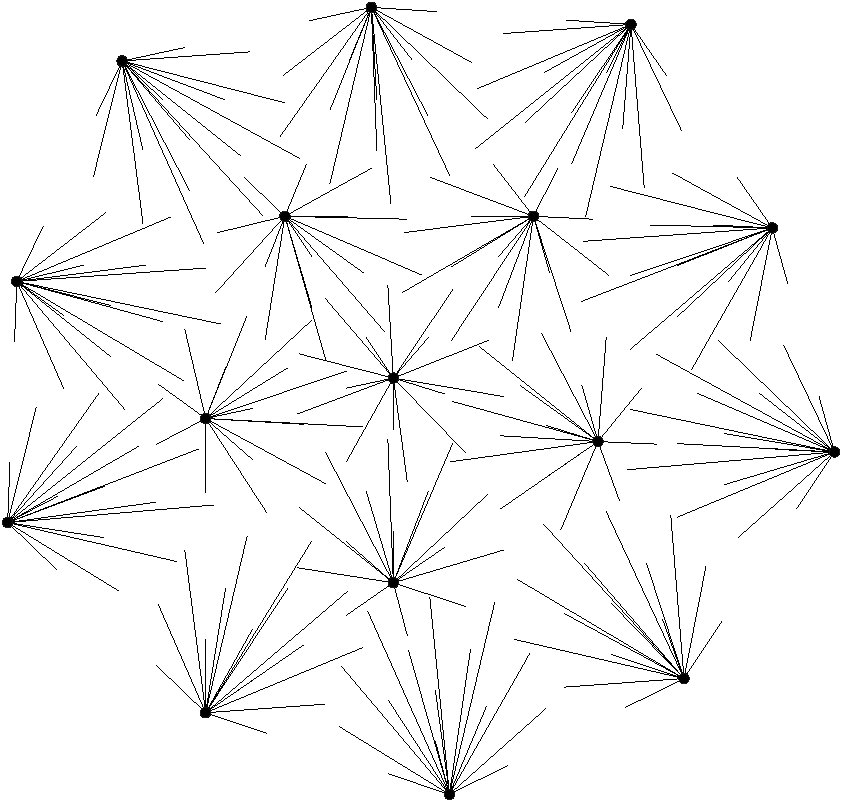
\includegraphics[width=.3\textwidth]{./figures/K16PEDCropped.pdf}
  \caption{Partial drawing of $K_{16}$}
  \label{fig: K_16}
\end{figure}


Bruckdorfer et.\ al.~\cite{Bruckdorfer} have shown that the upper bound on the number of vertices of a complete graph that can be drawn as a partial drawing is finite. They started with a simple proof that it is not possible to draw a partial drawing of a complete graph on 17 vertices in one-sided convex position. According to the result of Erd\H{o}s and Szekeres~\cite{Erdos}, any set with more than
\begin{equation*}
  \binom{2k-4}{k-2}
\end{equation*}
points, contains a subset in the one-sided convex position with $k$ points. If we insert $k = 17$ into the above expression, we arrive at the first estimate that for each
$$
  n > \binom{30}{15} = 155117520
$$
we cannot draw a partial drawing of a complete graph on $n$ vertices. They then significantly improved this estimate using the coordinate division of the plane on which the vertices of the complete graph are drawn into rectangles and showed that it is not possible to draw a partial drawing of the complete graph on 241 or more vertices.

In this work, we improve the estimate by a factor of more than two. We show that it is not possible to draw a partial drawing of the complete graph on 102 or more vertices. The main ideas are two. First, we use a different division of the plane on which the points of the graph are located. The coordinate division into rectangles has no real connection with the geometry of the partial drawing. Our approach to finding a suitable division was based on rays from pre-selected points of the drawing. In this way, the boundaries of the division are parallel to at least one of the partial edges. The resulting division has a geometry that is similar to the geometry of the partial drawing. However, the division now depends on the relative position of the pre-selected boundary points. The second idea is to analyze the entire drawing of the graph according to the location of three, sometimes even four, points of the drawing and not only two as in the previous estimates.

% TODO
In the next chapter, Preliminaries, we first define the basic concepts and establish terminology and notation. More important terms are indicated by the headings of the sections in which we define these terms. We then present the main tools (that follow from the fact that the graph $K_{3,3}$ is not planar), which allow us to control the number of points of a partial drawing. We prove the claims and theorems that serve as building blocks in the construction of the estimates.

In the third chapter, Estimates, we first define the frame in which all the points of the partial drawing lie. The frame is divided according to the three pre-selected boundary points into the following regions:
\begin{itemize}
  \item central triangle,
  \item left and right triangle and
  \item lower quadrilateral.
\end{itemize}
For each region, we derive an upper bound on the number of points in the partial drawing that lie in this region. We can assume that the central triangle is equilateral and use symmetry several times, which makes it easier to arrive at an estimate. It is different with the remaining areas. The left and right triangles are divided into cells so that each cell contains at most one point of the partial drawing. The position and number of these cells, however, vary according to the position of the selected boundary point. In addition to the cells, we use other types of polygons to divide the lower quadrilateral, which again depend on the position of the selected boundary point.

In the final chapter, Conclusion, we combine the derived bounds into the final result and present it graphically. Due to the dependence of the division on the mutual position of the boundary points, the result of the analysis is a function that represents the estimate for the upper bound on the maximum possible number of points of partial drawing. The illustrations show the division of the frame in the critical position of the boundary points, where this function reaches a maximum. We evaluate the result and suggest possible further guidelines for analysis. Appendix A provides the source code of the major calculations that helped us make the estimates.

\chapter{Preliminaries}
In this work we use only the Euclidean distance, the adjective Euclidean will be omitted. We consider finite sets of points $\Pi$ in the plane with certain constraints and want to estimate the maximum possible number of points. So we need some definitions. With $\quadsym{abcd}$ we denote a convex quadrilateral with vertices $a,b,c,d$, which follow each other in this order along its edges. If the sides of a convex quadrilateral are parallel to the coordinate axes, we use a more precise notation $\rectansym{abcd}$. We denote by $\trisym{abc}$ the triangle with vertices $a,b,c$. The length of line segment determined by the points $x,y$ is denoted by $|xy|$.

\begin{definition}
We say that a family of nonempty convex polygons
$$
  \mathcal{C} = \left\{ C_{1}, C_{2}, ..., C_{k} \right\},
$$
is a \textit{geometric partition} of polygon $L$, if
$$
  L = C_{1} \cup C_{2} \cup ... \cup C_{k}
$$
and for any $C_{i}, C_{j}, i \neq j$, intersection $C_{i} \cap C_{j}$ is considered to be a part of their common edge.
\end{definition}

\section{Ray coordinate system}
In the next chapter, we observe several times the position of the points depending on the position of up to three pre-selected points $x, y, z$. For any point $p$ located at an acute angle $\sangle{xzy}$, see Figure~\ref{fig: rays-coordinate-system}, we are interested in where the ray from the point $z$ trough the point $p$ intersects the line segment $\overline{xy}$ and at what ``height'' is the point $p$ from the position of the point $z$. Therefore, we introduce an alternative coordinate system.

\begin{figure}
\begin{center}
\begin{tikzpicture}[scale = 6.5, node distance=0.1cm,>=latex, dot/.style={circle,inner sep=1pt,fill,label={#1}, name=#1},
  extended line/.style={shorten >=-#1,shorten <=-#1},
 extended line/.default=1cm]

\begin{footnotesize}
\node [dot=](x) at (0,0) {};
\node [left = of x] {$x$};
\node [dot=](y) at (1,0) {};
\node [right = of y] {$y$};
\node [dot=](z) at ({1/2},{-sqrt(3)/2}) {};
\node [below = of z] {$z$};

% ticks on axes and mesh zx
\draw [thin] (0.3825000000, -0.6451889258) -- (0.3675000000, -0.6538491799);
\draw [thin] (0.2575000000, -0.4286825749) -- (0.2425000000, -0.4373428289);
\draw [thin] (0.1325000000, -0.2121762239) -- (0.1175000000, -0.2208364780);
\coordinate (zx1) at (0.3750000000,-0.6495190528);
\node [left = of zx1] {$\frac{1}{4}$};
\coordinate (zx2) at (0.2500000000,-0.4330127019);
\node [left = of zx2] {$\frac{1}{2}$};
\coordinate (zx3) at (0.1250000000,-0.2165063509);
\node [left = of zx3] {$\frac{3}{4}$};
\draw [thin, dotted] (zx1) -- (0.6250000000,-0.6495190528);
\draw [thin, dotted] (zx2) -- (0.7500000000,-0.4330127019);
\draw [thin, dotted] (zx3) -- (0.8750000000,-0.2165063509);

% ticks on axes and mesh xy
\draw [thin] (0.2500000000, 0.008660254038) -- (0.2500000000, -0.008660254038);
\draw [thin] (0.5000000000, 0.008660254038) -- (0.5000000000, -0.008660254038);
\draw [thin] (0.7500000000, 0.008660254038) -- (0.7500000000, -0.008660254038);
\draw [thin,dotted] (z) -- (-0.1666666667, 0.2886751346);
\draw [thin,dotted] (z) -- (0.1666666667, 0.2886751346);
\draw [thin,dotted] (z) -- (0.5000000000, 0.2886751346);
\draw [thin,dotted] (z) -- (0.8333333333, 0.2886751346);
\draw [thin,dotted] (z) -- (1.166666667, 0.2886751346);
\coordinate (xy1) at (0.2500000000,-0.0);
\node [below = of xy1,fill=white] {$\frac{1}{4}$};
\coordinate (xy2) at (0.5000000000,-0.0);
\node [below = of xy2,fill=white] {$\frac{1}{2}$};
\coordinate (xy3) at (0.7500000000,-0.0);
\node [below = of xy3,fill=white] {$\frac{3}{4}$};

% vectors and points
\draw [thin, ->] (x) -- (y);
\draw [thin, ->] (z) -- (x);
\node [dot=](p) at (0.875, 0.216506) {};
\node [above = of p,fill=white] {$p\langle \alpha, \beta \rangle$};
\node [dot=](q) at (0.3750000000, -0.4330127019) {};
\node [above = of q,fill=white] {$q\langle \frac{1}{4}, \frac{1}{2} \rangle$};

\end{footnotesize}
\end{tikzpicture}

\end{center}
\caption{Ray coordinate system.}
\label{fig: rays-coordinate-system}
\end{figure}

\begin{definition}[Ray coordinate system]
Let $x, y, z \in \mathbb{R}^{2}$ be fixed nonlinear points. Any point $p \in \mathbb{R}^{2}$ can be expressed as a linear combination of vectors $\vec{xy}$ and $\vec{zx}$ in the following way

\begin{equation*}
 \label{lin}
 \vec{zp} = \alpha \cdot \beta \cdot \vec{xy} + \beta \cdot \vec{zx}, \alpha, \beta \in \mathbb{R}
\end{equation*}

In \textit{ray coordinate system (RCS)} with respect to $x,y,z$ any point $p$ in the plane is determined by the ordered pair $(\alpha, \beta)$ and we write $p \langle \alpha, \beta \rangle$. The point $z$ is called \textit{origin} and the ray from $z$ through $x$ is called \textit{ray axis}. The third point that determines the RCS is $y$. The first coordinate $\alpha$ is called \textit{ray angle} and the second coordinate $\beta$ is called \textit{ray height} of the point $p$. Half-line with the starting point in $z$ passing through a point with ray angle $\xi$ is called a \textit{$\xi$-ray}.
\label{Ray coordinate system}
\end{definition}

For example, if $\vec{zq} = \frac{1}{2}(\frac{1}{4}\vec{xy} + \vec{zx})$ holds, the point $q$ has ray coordinates $q\langle \frac{1}{4}, \frac{1}{2} \rangle$ in RCS with respect to $x,y,z$.

\begin{definition}[Ray trapezoid]
In the ray coordinate system with respect to points $x, y, z$ the \textit{ray trapezoid}
$$
\tpz{\left[ \alpha,\omega,\gamma,\delta \right]_{x,y,z} }
$$
is trapezoid with vertices $\langle\alpha, \gamma\rangle, \langle\omega, \gamma\rangle, \langle\omega, \delta\rangle, \langle\alpha, \delta\rangle$, located in a convex angle $\sangle{xzy}$, see Figure~\ref{fig: ray-trapezoid}. Ray Trapezoid $\tpz{\left[ \alpha,\omega,\gamma,\delta \right]_{x,y,z} }$ corresponds to the Cartesian product
$$
\left[ \alpha,\omega \right] \times \left[ \gamma,\delta \right].
$$
The opposite sides of the trapezoid contained in the $z$-rays are called \textit{legs}, and the other two sides, which are parallel to the line segment $\overline{xy}$, are called \textit{bases}. The one closer to $z$ is called {\it short base} and the one farther away from $z$ is called {\it long base}. We have implicitly assumed that $\alpha \leq \omega$ and $\gamma \leq \delta$.
\end{definition}

\begin{figure}
\begin{center}
  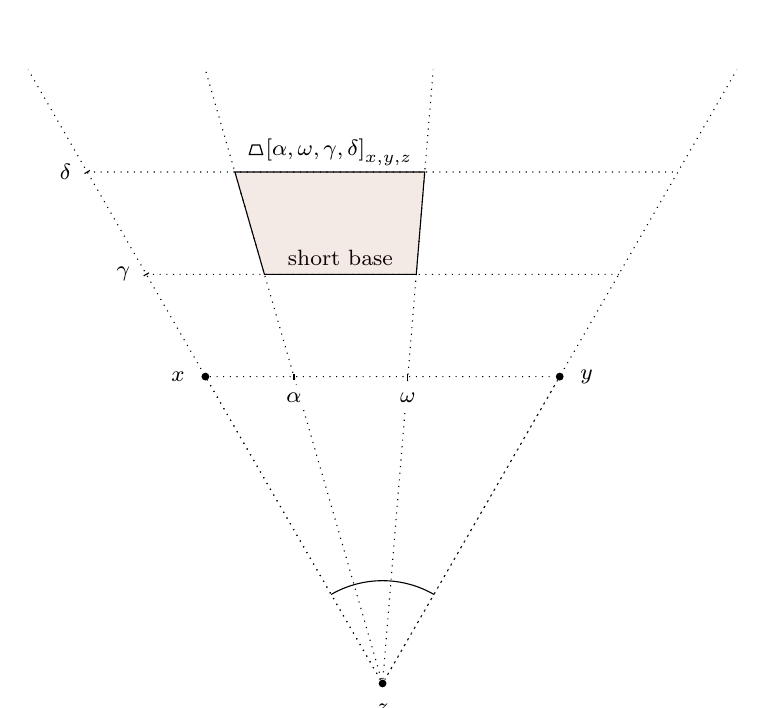
\begin{tikzpicture}[scale = 4.5, node distance=0.1cm,>=latex, dot/.style={circle,inner sep=1pt,fill,label={#1}, name=#1},
  extended line/.style={shorten >=-#1,shorten <=-#1},
 extended line/.default=1cm]
\begin{footnotesize}
\node [dot=](x) at (0,0) {};
\node [left = of x] {$x$};
\node [dot=](y) at (1,0) {};
\node [right = of y] {$y$};
\node [dot=](z) at ({1/2},{-sqrt(3)/2}) {};
\node [below = of z] {$z$};

\coordinate (x1) at (0.166667, 0.288675) {};
\coordinate (y1) at (0.595238, 0.288675) {};
\coordinate (y2) at (0.619048, 0.57735) {};
\coordinate (x2) at (0.0833333, 0.57735) {};

\draw[font=\footnotesize] (x1)--(y1) node[pos=0.5,above] {short base};

\fill[red, opacity=0.1] (0.166667, 0.288675) -- (0.595238, 0.288675) -- (0.619048, 0.57735) -- (0.0833333, 0.57735) -- (0.166667, 0.288675) -- cycle;
\draw [] (x1) -- (y1) -- (y2) -- (x2) -- (x1) -- cycle;

% rays
\draw [thin,dotted] (z) -- (-0.5, 0.866025);
\draw [thin,dotted] (z) -- (1.5, 0.866025);
\draw [thin,dotted] (z) -- (0., 0.866025);
\draw [thin,dotted] (z) -- (0.642857, 0.866025);

% ticks on y-axis
\draw [thin] (-0.174167, 0.284345) -- (-0.159167, 0.293005);
\draw [thin] (-0.340833, 0.57302) -- (-0.325833, 0.58168);

\coordinate (zx1) at (-0.166667, 0.288675);
\node [left = of zx1] {$\gamma$};
\draw [thin,dotted] (zx1) -- (1.16667, 0.288675);

\coordinate (zx2) at (-0.333333, 0.57735);
\node [left = of zx2] {$\delta$};
\draw [thin,dotted] (zx2) -- (1.33333, 0.57735);


% ticks on x-axis
\draw [thin] (0.2500000000, 0.008660254038) -- (0.2500000000, -0.008660254038);
\coordinate (xy1) at (0.2500000000,-0.0);
\node [below = of xy1,fill=white] {$\alpha$};

\draw [thin] (0.571429, 0.00866025) -- (0.571429, -0.00866025);
\coordinate (xy2) at (0.571429,0);
\node [below = of xy2,fill=white] {$\omega$};

%\draw [thin, ->] (x) -- (y);
%\draw [thin, ->] (z) -- (x);
\draw [thin,dotted] (x) -- (y) -- (z) -- (x) -- cycle;
%\node [above = of y2,fill=white] {$y_{2}$};
%\node [above = of x2,fill=white] {$x_{2}$};
%\node [below = of x1,fill=white] {$x_{1}$};
%\node [below = of y1,fill=white] {$y_{1}$};


%\tkzLabelAngle[pos=0.2,fill=white](x,z,y){$\angle xzy$}
\tkzMarkAngle[size=0.29 cm](y,z,x) %,mkcolor=red

\coordinate (q) at (0.35, 0.55) {};
\node [above = of q] {$\tpz{\left[ \alpha,\omega,\gamma,\delta \right]_{x,y,z} }$};

\end{footnotesize}
\end{tikzpicture}

\end{center}
\caption{Ray trapezoid in ray coordinate system with respect to $x,y,z$.}
\label{fig: ray-trapezoid}
\end{figure}

\section{Partial drawing}
Let $\Pi$ be the finite set of points in the plane and $n = |\Pi|$. For each pair of points $uv \in \Pi$, draw the line segment $\overline{uv}$, omitting the central half. The initial quarter of the line $\overline{uv}$, which contains the vertex $u$, is called a \textit{stub} from $u$ to $v$ and is denoted by $\overline{u}v$. The point $u$ is also called the \textit{start} of the stub $\overline{u}v$, and the other end of the stub its \textit{end}. The union of the two stubs $\overline{u}v$ and $\overline{v}u$ is called a \textit{partial edge} between the points $u$ and $v$. If any two partial edges intersect only at their possible common starting vertex, the resulting structure is called a \textit{partial drawing of a complete graph} $K_{n}$, and the set of points $\Pi$ its \textit{basis}. Let's write it more formally.

\begin{figure}
\input{./tikz/partial-edges.subfig}
\caption{How to draw a partial edge.}
\label{fig: partial-edges}
\end{figure}

\begin{definition}[Stubs]
Given points $u, v$ in the plane, line segment with ends $u$ and $\frac{3}{4}u + \frac{1}{4}v$ is called a \textit{stub} $\overline{u}v$, see Figure~\ref{fig: partial-edge}. Points $u$ and $\frac{3}{4}u + \frac{1}{4}v$ are called \textit{start} and \textit{end} of the stub $\overline{u}v$ respectively, see Figure~\ref{fig: stub-ends}. The end of the stub $\overline{u}v$ is denoted by $u_{v}$.
\label{def: stubs}
\end{definition}

\begin{definition}[Partial edge]
\textit{Partial edge} between the points $u, v$ is the union of the two stubs $\overline{u}v$ and $\overline{v}u$.
\label{def: partial-edge}
\end{definition}

\begin{definition}[Partial drawing]
Let $\Pi$ be the finite set of points in the plane and $n = |\Pi|$. The union of partial edges between all pairs of points in $\Pi$ is denoted by $\mathcal{D}(\Pi)$.

\begin{equation}
\mathcal{D}(\Pi) = \bigcup_{u,v \in \Pi} (\overline{u}v \cup \overline{v}u)
\end{equation}

If any two partial edges $(\overline{u}v \cup \overline{v}u)$ and $(\overline{u'}v' \cup \overline{v'}u'), u,v,u',v' \in \Pi$ intersect only at their possible common start (say $u = u'$), the resulting structure $\mathcal{D}(\Pi)$ is called \textit{partial drawing of a complete graph} $K_{n}$. The set of points $\Pi$ is called its \textit{basis}.
\label{def: partial-drawing}
\end{definition}

\begin{figure}
\centering
\input{./tikz/drawings-of-K6.subfig}
\caption{Various drawings of $K_{6}$.}
\label{fig: drawings-of-K6}
\end{figure}

An example is in Figure~\ref{fig: drawing-of-K_6}. The same graph was drawn with partial edges in Figure~\ref{fig: wrong-drawing-of-K_6}. We notice that we are violating the non-crossing requirement. The same graph can be drawn with partial edges without crossings, if the points are moved accordingly, see Figure~\ref{fig: partial-drawing-of-K_6}. Such a drawing is called \textit{partial drawing of a complete graph} $K_{6}$.

It is easy check that the basis points of partial drawing are in a general position.
\begin{lemma}[Non-linearity]
If $\Pi$ is the basis of a partial drawing of a complete graph, then $\Pi$ does not contain three collinear points.
\end{lemma}
\begin{proof}
Suppose that the set $\Pi$ contains collinear points $u, v, w$. If the point $v$ lies strictly between $u$ and $w$, the stub $\overline{u}v$ is contained in stub $\overline{u}w$. This is not possible in a partial drawing.
\label{lemma: non-linearity}
\end{proof}

For each potential basis $\Pi$ of the partial drawing, we will assume that it does not contain three collinear points.

When estimating the number of points in a partial drawing of a complete graph, we will be interested in whether for two points from some region must come to a crossing between the stubs to three pre-selected points. Therefore, we introduce the term {\it umbrella}.

\begin{definition}[Umbrella]
Let $x, y, z$ be points in general position. For any point $p$, an \textit{umbrella} $Y_{p,x,y,z}$ of the point $p$ is a union of $x, y, z$ stubs:
\begin{equation*}
Y_{p,x,y,z} = \overline{p}x \cup \overline{p}y \cup \overline{p}z.
\end{equation*}
\label{umbrella}
\end{definition}

In Figure~\ref{fig: umbrella-no-crossings} is an example without crossings between the umbrellas of points $u$ and $v$ with respect to three pre-selected points that are not part of the Figure. Figures~\ref{fig: umbrella-crossings-1} and ~\ref{fig: umbrella-crossings-2} show examples of crossings between umbrellas.

\begin{figure}
\centering
\input{./tikz/umbrella-crossings.subfig}
\caption{Possible crossings of umbrellas.}
\label{fig: umbrella-crossings}
\end{figure}

Let point $p$ have ray coordinates $p = \langle\beta, \delta\rangle$, then we can calculate the ray coordinates of the ends of the umbrella $Y_{p,x,y,z}$:
\begin{align}
  \label{eq: ray-coordinates-umbrella-1}
  p_{x} &= \left\langle \frac{3\delta\beta}{1+3\delta}, \frac{1+3\delta}{4} \right\rangle,\\[6pt]
  \label{eq: ray-coordinates-umbrella-2}
  p_{y} &= \left\langle\ \frac{1+3\delta\beta}{1+3\delta}, \frac{1+3\delta}{4} \right\rangle,\\[6pt]
  p_{z} &= \left\langle \beta, \frac{3}{4}\delta \right\rangle.
\end{align}


\begin{corollary}
\label{cor: consequence-of-ray-coordinates-of-umbrella-ends}
Select RCS with respect to $x,y,z$ and let the ray angle $\beta \in (0,1)$ be fixed. With increasing ray height $\delta \geq 0$ is
$$
\frac{3\delta\beta}{1+3\delta}
$$
an increasing function of height $\delta$ and
$$
\frac{1+3\delta\beta}{1+3\delta}
$$
a decreasing function of height $\delta$. This means that at a fixed angle $\beta$, with increasing height, the ray angle of the end $p_{x}$ decreases and the ray angle of the end $p_{y}$ increases.
\end{corollary}

We now define ray trapezoids with certain properties as additional terminology for determining the upper bound in the next section.

\begin{definition}[Shadows]
In ray coordinate system with respect to points $x,y,z$ the \textit{shadows} $S_{\overline{x}y}$ and $S_{\overline{y}x}$ are ray trapezoids
$$
S_{\overline{x}y} = \tpz{\left[ 0,\frac{1}{4},1,\frac{4}{3} \right]_{x,y,z} }
$$
and
$$
S_{\overline{y}x} = \tpz{\left[ \frac{3}{4},1,1,\frac{4}{3} \right]_{x,y,z} }.
$$
\end{definition}

\begin{proposition}
For $x,y,z \in \Pi$, the following obviously holds
\begin{equation}
\left( S_{\overline{x}y} \setminus \left\{ x \right\} \right) \cap \Pi = \emptyset
\end{equation}
and
\begin{equation}
\left( S_{\overline{y}x} \setminus \left\{ y \right\} \right) \cap \Pi = \emptyset.
\end{equation}
\end{proposition}

\begin{proof}
For each  $p \in S_{\overline{x}y}$ or $p \in S_{\overline{y}x}$ the stub $\overline{p}z$ intersects the short base of shadow $S_{\overline{x}y}$ or shadow $S_{\overline{y}x}$. The short base of the shadow $S_{\overline{x}y}$ is the stub $\overline{x}y$ and the short base of the shadow $S_{\overline{y}x}$ is the stub $\overline{y}x$, therefore $p \notin \Pi\setminus \left\{ x,y \right\}$.
\end{proof}

\begin{definition}[Layer]
In ray coordinate system with respect to points $x,y,z$ the \textit{layer} $L$ is the ray trapezoid
$$L = \tpz{\left[ \alpha,\omega,\gamma,\delta \right]_{x,y,z} },$$
for which
$$
\gamma \geq \frac{3}{4} \cdot \delta.
$$
The parameters $\gamma$ and $\delta$ are called \textit{lower} and \textit{upper} height of the layer $L$. The parameters $\alpha$ and $\omega$ are called \textit{left} and \textit{right} border of the layer $L$.
\end{definition}

The consequence of the condition $\gamma \geq \frac{3}{4}\delta$ is that for any point $p \in L$ the stub $\overline{p}z$ intersects short base of the layer $L$. (Even more applies, the stub $\overline{p}z$ intersects the line parallel to the line segment $\overline{xy}$ at the height $\frac{3}{4}\delta$.)

\begin{figure}
\begin{center}
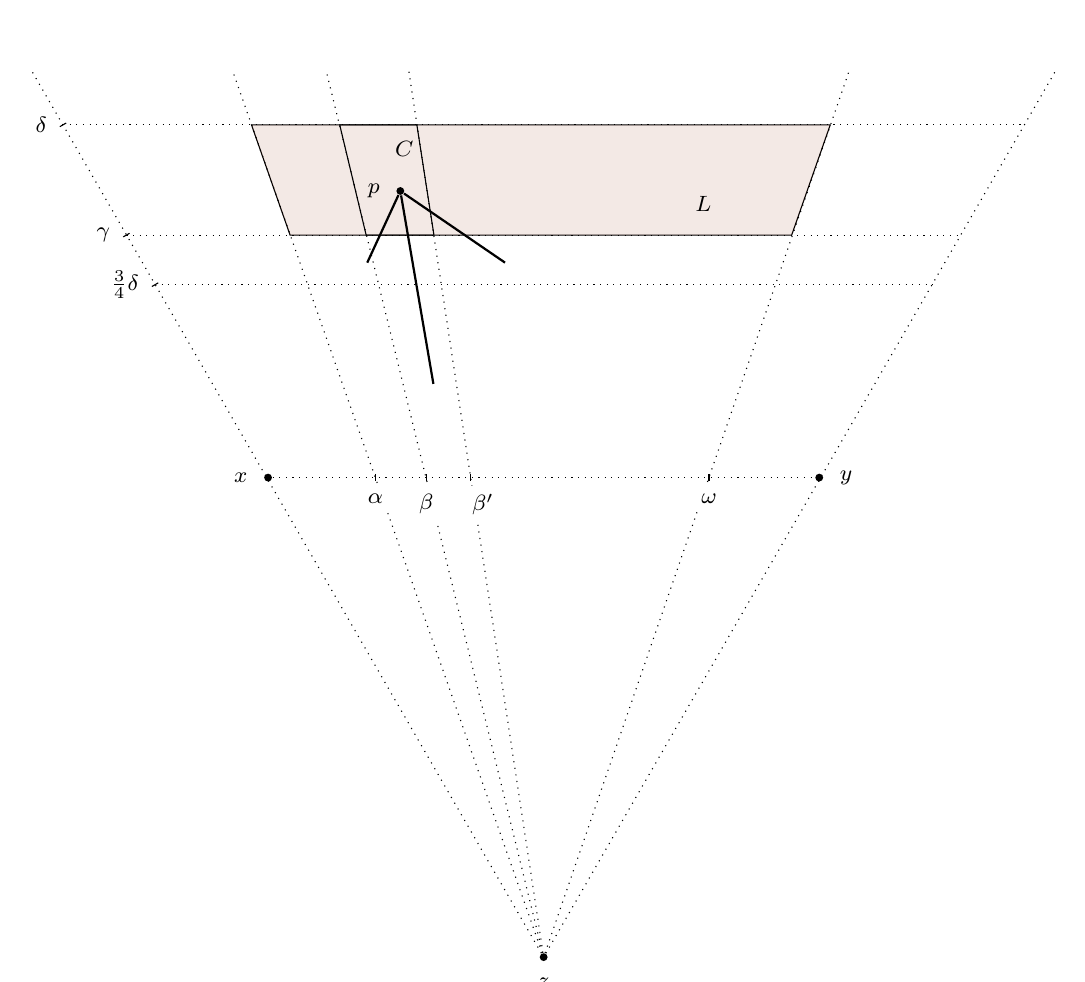
\begin{tikzpicture}[scale = 7, node distance=0.1cm,>=latex, dot/.style={circle,inner sep=1pt,fill,label={#1}, name=#1},
dot2/.style={circle,inner sep=1pt,draw,fill=white,label={#1}, name=#1}]
\begin{footnotesize}
\node [dot=](x) at (0,0) {};
\node [left = of x] {$x$};
\node [dot=](y) at (1,0) {};
\node [right = of y] {$y$};
\node [dot=](z) at (0.5,-0.87) {};
\node [below = of z] {$z$};

% triangle xyz
\draw [thin,dotted] (x) -- (y);

% band L
\draw[] (-0.03,0.64) -- (1.02,0.64) -- (0.95,0.44) -- (0.04,0.44) -- (-0.03,0.64) -- cycle;

\fill[red, opacity=0.1] (-0.03,0.64) -- (1.02,0.64) -- (0.95,0.44) -- (0.04,0.44) -- (-0.03,0.64) -- cycle;

\node [dot=](p) at (0.24,0.52) {};
\node [left = of p] {$p$};
\coordinate (px) at (0.18,0.39) {};
\coordinate (py) at (0.43,0.39) {};
\coordinate (pz) at (0.3,0.17) {};

\coordinate (xp) at (0.06,0.13) {};
\coordinate (yp) at (0.81,0.13) {};
\coordinate (zp) at (0.43,-0.52) {};

\draw [thick] (p) -- (px);
\draw [thick] (p) -- (py);
\draw [thick] (p) -- (pz);

%\draw [thick] (x) -- (xp);
%\draw [thick] (y) -- (yp);
%\draw [thick] (z) -- (zp);

%%%%%%%%%%%%%%%%%%%%%%%%%%%%%%%%%%%%%%%%%%%%%%5
%% horizontal ticks, dashed lines
\draw [thin] (-0.199231,0.353331) -- (-0.210769,0.346669);
\draw [thin] (-0.251231,0.443331) -- (-0.262769,0.436669);
\draw [thin] (-0.366231,0.643331) -- (-0.377769,0.636669);
\coordinate (delta) at (-0.372,0.64);
\node [left = of delta] {$\delta$};
\coordinate (gamma) at (-0.257,0.44) {};
\node [left = of gamma] {$\gamma$};
\coordinate (gammakaca) at (-0.205,0.35) {};
\node [left = of gammakaca] {$\frac{3}{4}\delta$};

\coordinate (delta1) at (1.372,0.64) {};
\coordinate (gamma1) at (1.257,0.44) {};
\coordinate (gammakaca1) at (1.205,0.35) {};
\draw [thin,dotted] (delta) -- (delta1);
\draw [thin,dotted] (gamma) -- (gamma1);
\draw [thin,dotted] (gammakaca) -- (gammakaca1);

%%%%%%%%%%%%%%%%%%%%%%%%%%%%%%%%%%%%%%%%%%%%%%%%%%
%% vertical ticks
\draw [thin] (0.195,0.00666173) -- (0.195,-0.00666173); % alpha
\draw [thin] (0.8,0.00666173) -- (0.8,-0.00666173); % beta
\draw [thin] (0.287, 0.00666173) -- (0.287, -0.00666173); % alphai
\draw [thin] (0.367, 0.00666173) -- (0.367, -0.00666173); % alphaii

\coordinate (alpha) at ({0.2-0.005},0) {};
\coordinate (beta) at (0.8,0) {};
\coordinate (alphai) at ({0.29 - 0.003},0) {};
%\coordinate (alphaii) at ({0.37 - 0.003},0) {};
\coordinate (alphaii) at ({0.39},0) {};

\coordinate (z1) at (-0.43,0.74) {};
\coordinate (z2) at (-0.065,0.74) {};
\coordinate (z3) at ({0.11 - 0.005},0.74) {};
\coordinate (z4) at ({0.25 + 0.005},0.74) {};
\coordinate (z5) at ({1.05 + 0.005},0.74) {};
\coordinate (z6) at (1.43,0.74) {};
% narisemo zarke
\draw [thin,dotted] (z) -- (z1);
\draw [thin,dotted] (z) -- (z2);
\draw [thin,dotted] (z) -- (z3);
\draw [thin,dotted] (z) -- (z4);
\draw [thin,dotted] (z) -- (z5);
\draw [thin,dotted] (z) -- (z6);


\node [below = of alpha,fill=white] {$\alpha$};
\node [below = of beta,fill=white] {$\omega$};
\node [below = of alphaii,fill=white] {$\beta'$};
\node [below = of alphai,fill=white] {$\beta$};

%\node [dot2=](ue) at (0.2,0.35) {};
%\coordinate (uee) at (0.19, 0.35) {};
%\node [below = of uee,fill=white] {$\undersym{e}$};
%\coordinate (uff) at (0.33,0.35) {};
%\node [dot2=](uf) at (0.315,0.35) {};
%\node [below = of uff,fill=white] {$\undersym{f}$};
%
\coordinate (e) at (0.178,0.44) {};
\coordinate (f) at (0.301,0.44) {};
%\coordinate (ee) at (0.18,0.413) {};
%\coordinate (ff) at (0.29, 0.413) {};
%\node [left = of ee] {$e$};
%\node [right = of ff] {$f$};
%
\coordinate (g) at (0.27,0.64) {};
%\node [above = of g,fill=white] {$g$};
\coordinate (h) at (0.13,0.64) {};
%\node [above = of h,fill=white] {$h$};

\draw (e) -- (f) -- (g) -- (h) -- (e) -- cycle;
\coordinate (pasL) at (0.79, 0.54) {};
\node [below = of pasL] {$L$};


\coordinate (pasL) at (0.247, 0.64) {};
\node [below = of pasL] {$C$};

\end{footnotesize}
\end{tikzpicture}

\end{center}
\caption{Maximal cell $C$ in layer $L$.}
\label{fig: layer-L}
\end{figure}

\begin{definition}[Cell]
In ray coordinate system with respect to points $x,y,z$ the \textit{cell} $C$ is ray trapezoid
$$
C = \tpz{\left[ \beta,\beta',\gamma,\delta \right]_{x,y,z} }
$$
in the layer $L = \tpz{\left[ \alpha,\omega,\gamma,\delta \right]_{x,y,z} }$, where for any point $p \in C$ holds:
\begin{itemize}
  \item stub $\overline{p}x$ intersects $\beta$-ray;
  \item stub $\overline{p}y$ intersects $\beta'$-ray;
  \item stub $\overline{p}z$ intersects short base of the cell $L$.
\end{itemize}
Parameters $\beta$ and $\beta'$ are called \textit{left} and \textit{right} border of the cell $C$.
\end{definition}

% first relationship: p = <beta', delta>
Stub $\overline{p}z$ intersects the short base due to the relationship between the lower and upper height of the layer $L$.
Let us find the relationships between the left and right borders $\beta$ and $\beta'$ in cell $C$. According to~\eqref{eq: ray-coordinates-umbrella-1} and~\eqref{eq: ray-coordinates-umbrella-2} it holds
$$
\beta' \leq \frac{(1+3\delta)\beta}{3\delta}
$$
and
$$
\beta' \leq \frac{1+3\delta\beta}{1+3\delta}.
$$

\begin{definition}
Cell $C = \tpz{\left[ \beta,\beta',\gamma,\delta \right]_{x,y,z} }$ in layer $L = \tpz{\left[ \alpha,\omega,\gamma,\delta \right]_{x,y,z} }$ is \textit{maximal}, if for any interval
$$
I = \left[ \xi, \xi' \right],
$$
for which
$$
\left[ \beta, \beta' \right] \subsetneq \left[ \xi, \xi' \right],
$$
the ray trapezoid $\tpz{\left[ \xi,\xi',\gamma,\delta \right]_{x,y,z} }$ is not a cell.
\end{definition}

This means that for the maximal cell $\tpz{\left[ \beta,\beta',\gamma,\delta \right]_{x,y,z} }$ holds
$$
\beta' = \frac{(1+3\delta)\beta}{3\delta} \text{\hspace{0.8cm}   and   \hspace{0.8cm}} \beta' \leq \frac{1+3\delta\beta}{1+3\delta}
$$
or
$$
\beta' = \frac{1+3\delta\beta}{1+3\delta} \text{\hspace{0.8cm}   and   \hspace{0.8cm}} \beta' \leq \frac{(1+3\delta)\beta}{3\delta}.
$$

\begin{proposition}
Denote
\begin{align}
\label{eq:f1_beta}
f_{1,\delta}(\beta) &= \frac{(1+3\delta)\beta}{3\delta},\\[6pt]
\label{eq:f2_beta}
f_{2,\delta}(\beta) &= \frac{1+3\delta\beta}{1+3\delta}.
\end{align}
If
$$
\beta' = \min\left\{ f_{1,\delta}(\beta), f_{2,\delta}(\beta) \right\},
$$
then the cell $C = \tpz{\left[ \beta,\beta',\gamma,\delta \right]_{x,y,z} }$ is maximal in layer $L$ with lower and upper layer height $\gamma$ and $\delta$.
\end{proposition}

\begin{figure}
\begin{center}
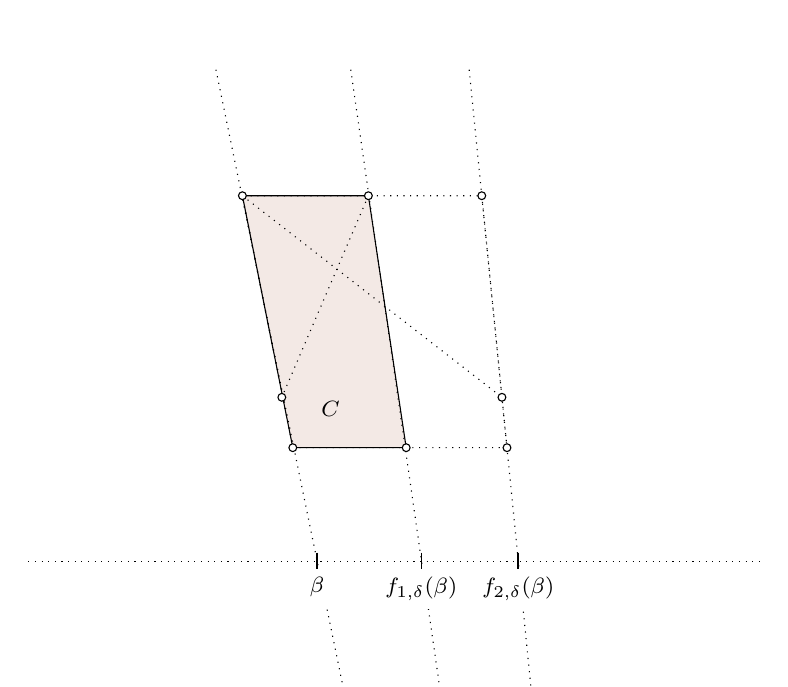
\begin{tikzpicture}[scale = 16, node distance=0.1cm,>=latex, dot/.style={circle,inner sep=1pt,fill,label={#1}, name=#1},
dot2/.style={circle,inner sep=1pt,draw,fill=white,label={#1}, name=#1}]
\begin{footnotesize}
\draw [dotted] (0,0.35) -- (0.58,0.35);


\coordinate (ue) at (0.21,0.44) {};
\coordinate (uf) at (0.3,0.44) {};
\coordinate (ff) at (0.38,0.44) {};
\coordinate (gx) at (0.2013,0.48) {};
\coordinate (hy) at (0.376,0.48) {};
\coordinate (h) at (0.17,0.64) {};
\coordinate (g) at (0.27,0.64) {};
\coordinate (gg) at (0.36,0.64) {};

\fill[red,opacity=0.1] (ue) -- (uf) -- (g) -- (h) -- (ue) -- cycle;

\draw (ue) -- (uf) -- (g) -- (h) -- (ue) -- cycle;
\draw [dotted] (g) -- (gx);
\draw [dotted] (h) -- (hy);
\draw [dotted] (ue) -- (ff) -- (gg) -- (h) -- cycle;

\coordinate (z3) at ({0.15 - 0.001},0.74) {};
\coordinate (zz3) at ({0.26 - 0.008},0.24) {};
\coordinate (z4) at ({0.26 - 0.004},0.74) {};
\coordinate (zz4) at ({0.33 - 0.002},0.24) {};
\coordinate (z5) at (0.35,0.74) {};
\coordinate (zz5) at (0.4,0.24) {};

\draw [dotted] (z3) -- (zz3);
\draw [dotted] (z4) -- (zz4);
\draw [dotted] (z5) -- (zz5);

\node [dot2=](ue) at (0.21,0.44) {};
\node [dot2=](uf) at (0.3,0.44) {};
\node [dot2=](ff) at (0.38,0.44) {};
\node [dot2=](gx) at (0.2013,0.48) {};
\node [dot2=](hy) at (0.376,0.48) {};
\node [dot2=](h) at (0.17,0.64) {};
\node [dot2=](g) at (0.27,0.64) {};
\node [dot2=](gg) at (0.36,0.64) {};

\draw [thin] (0.2292,{0.35 + 0.00666173}) -- (0.2292,{0.35-0.00666173}); % alphai
\coordinate (alphai) at (0.2292,0.35) {};
\node [below = of alphai,fill=white] {$\beta$};

\draw [thin] (0.312,{0.35+ 0.00666173}) -- (0.312,{0.35-0.00666173}); % alphaii
\coordinate (alphaii) at (0.312,0.35) {};
\node [below = of alphaii,fill=white] {$f_{1,\delta}(\beta)$};

\draw [thin] (0.3888,{0.35+ 0.00666173}) -- (0.3888,{0.35-0.00666173}); % alphaii
\coordinate (alphaiii) at (0.389,0.35) {};
\node [below = of alphaiii,fill=white] {$f_{2,\delta}(\beta)$};

\coordinate (Qi) at (0.24,0.49) {};
\node [below = of Qi] {$C$};

%\coordinate (Qii) at (0.313,0.49) {};
%\node [below = of Qii] {$Q_{i}'$};
\end{footnotesize}
\end{tikzpicture}

\end{center}
\caption{Example of functions $f_{1,\delta}(\beta), f_{2,\delta}(\beta)$ and corresponding maximal cell $C$.}
\label{fig: edge-layers-2}
\end{figure}

Compare functions $f_{1,\delta}(\beta)$ and $f_{2,\delta}(\beta)$.
\begin{proposition}
\label{prop: compare-functions-f1-f2}
If $\beta \in [0,1]$ and $\delta \geq \frac{4}{3}$, then
\begin{itemize}
  \item $f_{1,\delta}(\beta) \leq f_{2,\delta}(\beta)$, at $\beta \leq \frac{3\delta}{1 + 6\delta}$ and
  \item $f_{1,\delta}(\beta) \geq f_{2,\delta}(\beta)$, at $\beta \geq \frac{3\delta}{1 + 6\delta}$.
\end{itemize}
\end{proposition}

\begin{proof}
Expression $f_{1,\delta}(\beta) - f_{2,\delta}(\beta)$ has the same sign as $(1 + 3\delta) \cdot 3\delta \cdot (f_{1,\delta}(\beta) - f_{2,\delta}(\beta))$. Calculate
\begin{align*}
(1 + 3\delta) \cdot 3\delta \cdot (f_{1,\delta}(\beta) - f_{2,\delta}(\beta)) &= \\[6pt]%
= (1 + 3\delta)^{2} \cdot \beta - (1 + 3\delta\beta) \cdot 3\delta &= \\[6pt]%
= \beta \cdot (1 + 6\delta) - 3\delta, \\[6pt]%
\end{align*}
which is greater than zero exactly when $\beta \leq \frac{3\delta}{1+6\delta}$.
\end{proof}

% upper bound
\section{Upper bound}
Let $\Pi $ be the basis of a partial drawing of a complete graph. In the next section, we show that the power of the set $\Pi$ has an upper bound. This means that there are no partial drawings of complete graphs on arbitrarily large numbers of vertices. Without loss of generality, the following properties can be assumed for $\Pi$.

\begin{properties}
\leavevmode
\begin{itemize}
  \item[P1)] Diameter of $\Pi$ is equal to $1$.
  \item[P2)] The points $a$ and $b$ $\in \Pi$ at the maximum distance of $1$ in $\Pi$, have coordinates $(0,0)$ in $(1,0)$.
  \item[P3)] The point in $\Pi$ furthest from the $x$-axis has a positive $y$-coordinate denoted by $c$. (If there are more candidates, select one with the largest $x$-coordinate.)
  \item[P4)] The point in $\Pi$, with the smallest $y$-coordinate is denoted by $d$. (If there are more candidates, select one with the largest $x$-coordinate, even $d = b$ is possible.)
\end{itemize}
\label{list: properties}
\end{properties}

\begin{definition}[Frame]
\label{def: frame}
The frame $F$ of the drawing is the smallest coordinate rectangle containing all the points from $\Pi$. In Figure~\ref{fig: frame}, it's vertices are denoted by $\abovesym{a}, \undersym{a}, \abovesym{b}, \undersym{b}$. If we denote by $c_{y}$ and $d_{y}$ the $y$-coordinates of points $c$ and $d$, then
\begin{equation*}
F = {[0,1] \times [d_{y}, c_{y}]} =
\rectansym{\undersym{a}\undersym{b}\abovesym{b}\abovesym{a}}.
\end{equation*}
\end{definition}

\begin{figure}
\centering
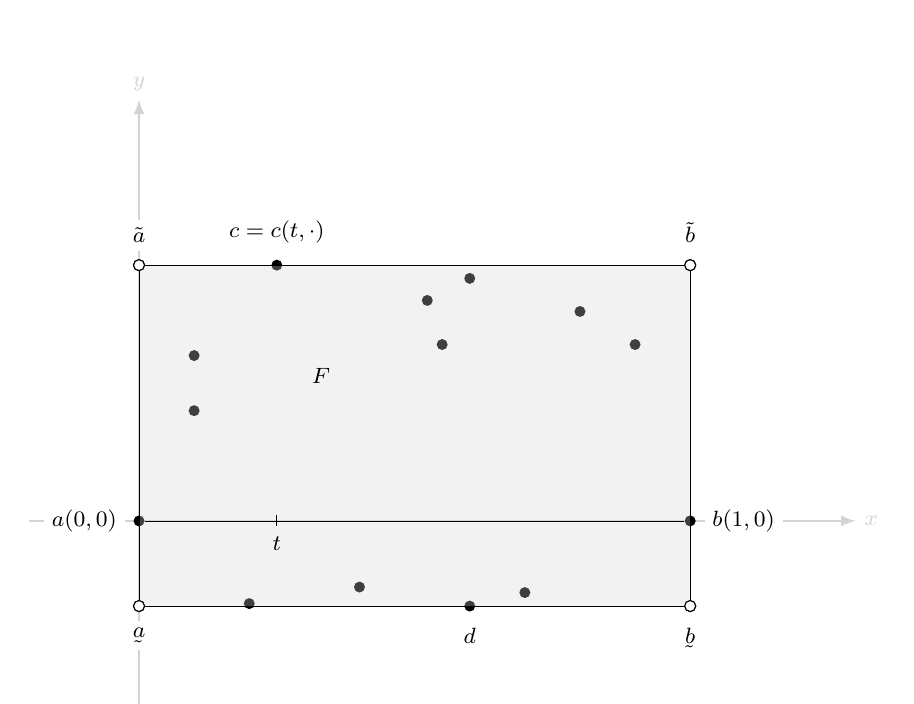
\begin{tikzpicture}[scale = 7, node distance=0.1cm,>=latex, dot/.style={circle,inner sep=1.4pt,fill,label={#1}, name=#1},
dot2/.style={circle,inner sep=1.4pt,draw,fill=white,label={#1}, name=#1}]
\begin{footnotesize}
% axes
\draw[gray,thick,->] ({-0.2}, 0) -- (1.3, 0) node[right] {$x$};
\draw[gray,thick,->] (0, {-0.1545-0.2}) -- ({0, 0.464+0.3}) node[above] {$y$};

\node [dot=] at (0.1,0.2) {};
\node [dot=] at (0.1,0.3) {};
\node [dot=] at (0.2,-0.15) {};
\node [dot=] at (0.4,-0.12) {};
\node [dot=] at (0.6,0.44) {};
\node [dot=] at (0.55,0.32) {};
\node [dot=] at (0.7,-0.13) {};
\node [dot=] at (0.523,0.4) {};
\node [dot=] at (0.8,0.38) {};
\node [dot=] at (0.9,0.32) {};

\node [dot=](a) at (0,0) {};
\node [dot=](b) at (1,0) {};
\node [dot=](c) at ({1/4},0.464) {};
\node [dot=](d) at ({3/5}, -0.1545) {};
\node [dot2=](abovea) at (0,0.464) {};
\node [dot2=](aboveb) at (1,0.464) {};
\node [dot2=](undera) at (0,-0.1545) {};
\node [dot2=](underb) at (1,-0.1545) {};

\fill[color-trapezoid,opacity=0.3] (0,0.464) -- (1,0.464)  -- (1,-0.1545) -- (0,-0.1545)-- cycle;

% c
\coordinate (t) at ({1/4},0);
\draw [thin] (-0.01, 0.464) -- (0.01, 0.464);
\coordinate (cy) at (0,0.464);

% d
\draw [thin] ({1/4}, 0.01000000000) -- ({1/4}, -0.01000000000);
\coordinate (u) at (0,-0.1545);

\draw[ultra thin] (undera) -- (underb) -- (aboveb) -- (abovea) -- (undera) -- cycle;
\draw[ultra thin] (a) -- (b) -- cycle;
\node [right = of b,fill=white] {$b(1,0)$};
\node [left = of a,fill=white] {$a(0,0)$};
\node [above = of c] {$c = c(t, \cdot)$} {};
\node [below = of d] {$d$}; 

\node [below = of t] {$t$};

\node [dot2=](abovea) at (0,0.464) {};
\node [dot2=](aboveb) at (1,0.464) {};
\node [dot2=](undera) at (0,-0.1545) {};
\node [dot2=](underb) at (1,-0.1545) {};
\node [above = of abovea,fill=white] {$\abovesym{a}$};
\node [above = of aboveb] {$\abovesym{b}$};
\node [below = of undera, fill=white] {$\undersym{a}$};
\node [below = of underb] {$\undersym{b}$};
\coordinate (f) at (0.33,0.22);
\node [above = of f] {$F$};
\end{footnotesize}
\end{tikzpicture}
\caption{Frame $F$}
\label{fig: frame}
\end{figure}

We would like to find the upper bound on the number of points in $\Pi$. Depending on the relative position of the points $c, d$ with respect to points $a, b$ we will construct the coverage $\mathcal{C}$ of the frame $F$ with a finite family of polygons $P_{1}, P_{2}, ..., P_{k}$:
$$
  F \subseteq P_{1} \cup P_{2} \cup ... \cup P_{k}.
$$

The shapes of the polygons $P_{i}$ and the number of polygons $k$ of coverage $\mathcal{C}$ will depend on the parameters $t$ and $h$:
\begin{align}
  \label{eq: t}
  t = c_{x}, \\[6pt]
  \label{eq: h}
  h = -\frac{d_{y}}{c_{y}}.
\end{align}

We denote by $c_{x}$ the $x$-coordinate of the point $c$. The point $c$ can be arbitrarily close to $\abovesym{a}$ or $\abovesym{b}$, so $t$ is any real number from the interval $(0, 1)$. The parameter $h$ is any real number from the interval $[0,1]$. We will estimate the upper bound on the number of possible basis points of the partial drawing located in each individual polygon. The estimate for the upper bound on the number of basis points in the polygon $P_{i}$ is denoted by $m(P_{i})$, so $|\Pi \cap P_{i}| \leq m(P_{i})$. The notation $m(P_{i}) = m_{0}$ means that we will be able to show that a maximum of $m_{0}$ points of a partial drawing can lie in the polygon $P_{i}$. The estimate $m(\mathcal{C}(t, h))$ of the upper bound on the number of all basis points of partial drawing of complete graph is obtained by summing the estimates of the upper bounds $m(P_{i}), i = 1, ..., k(t,h)$:
\begin{equation}
  \label{eq: estimate-for-F}
  m(\mathcal{C}(t,h)) = m(P_{1}) + m(P_{2}) + ... + m(P_{k(t,h)}).
\end{equation}

The parameters $t$ and $h$ change the shape of $k$ polygons $P_{i}$. To estimate the power of the partial drawing basis of complete graph, we must calculate for which pair $t, h$ the Estimate~\eqref{eq: estimate-for-F} is the worst.

\section{Step functions}
We define a \textit{step function} $ k = k (t) $ as a mapping
$$
  k: \left [0,1 \right] \mapsto \mathbb{N},
$$
which is
\begin{itemize}
\item piecewise constant and
\item there is a finite family of parameter values $t_{1}, t_{2}, ..., t_{r}$, where discontinuity can occur.
\end{itemize}

Additionally, $ k = k (t) $ is \textit{jump-step function} if it has a jump at each point of discontinuity. That means if
$$
  \lim_{t \to t_{0} ^{+}} k (t) \neq \lim_{t \to t_{0} ^{-}} k (t),
$$
then
$$
  k (t_{0}) = \lim_{t \to t_{0} ^{+}} k (t) \text{\hspace{0.8cm} or \hspace{0.8cm}} k (t_{0} ) = \lim_{t \to t_{0} ^{+}} k (t).
$$
A non-jump-step function may have values at a single point that differ from both the left and right limits.

To calculate the maximum of the step function, we need exact values of the discontinuity points. To calculate the maximum of the jump-step function, however, it is sufficient to know
\begin{itemize}
\item approximate values of discontinuity points $ (t_{i})_{i} $ and
\item an ascending sequence of rational numbers called \textit{system of safety intervals}:
$$
  q_{0} < q_{1} < ... < q_{r},
$$
for which for every $ i = 1, ..., r $ the inclusion
$$
  t_{i} \in (q_{i-1}, q_{i}).
$$
is fulfilled.
\end{itemize}

The maximum value of the jump-step  function $ k $ can be determined by calculating precisely the values of $k$ in all rational numbers $ q_{i}, i = 0, ..., r $.

The sum of step functions is obviously a step function, but the sum of jump-step functions is not necessarily jump-step function. If the jump-step functions $ k_{1} $ and $k_{2}$ have different points of discontinuity, then their sum $ k_{1} + k_{2} $ is also a jump-step function.

Since in practice we will know only the approximations of the discontinuity points of $ k_{1} $ and $ k_{2} $, we will be able to prove the jump of the sum $ k_{1} + k_{2} $ with their systems of safety intervals. If we find a sequence of rational numbers
$$ q_{0} <q_{1} <... <q_{r}, $$
for which holds that at each of the open intervals
$$ (q_{i-1}, q_{i}), i = 1, ..., r $$
at most one of the jump-step functions $ k_{1} $ or $ k_{2} $ has a jump, then $ k_{1} + k_{2} $ is also a jump-step function and its maximum can be calculated by calculating $ k_{1} (q_{i}) + k_{2} (q_{i}) $, for all $ i = 0, ..., r $.

In practice, we will determine the upper bound for some of the areas depending on the value of the parameter $t$. For region $P$, $k_{P}(t)$ is the upper limit for the number of points in the basis $P$, $|\Pi \cap P|$. For a global estimate, we could find a maximum for each area of $P$
$$
m(P) = \max_{t} \left \{k_{P}(t) \right \},
$$
but a better global estimate is obtained by summing the functions $k$ by individual regions and applying the maximum to the obtained sum. The functions $k = k_{P}(t)$ have natural numbers as values and only finitely many discontinuities.


\section{Crossing theorems}
The following are two theorems about crossings. In region $T_{0}$ defined in a ray trapezoid or in a triangle, we can effectively limit the number of basis points with the Theorem~\ref{thm: k33-trapezoid} or with the Theorem~\ref{thm: k33-triangle}. At this point we remind the reader that according to Lemma~\ref{lemma: non-linearity} none of the three points in $\Pi$ are collinear.

\begin{figure}
\centering
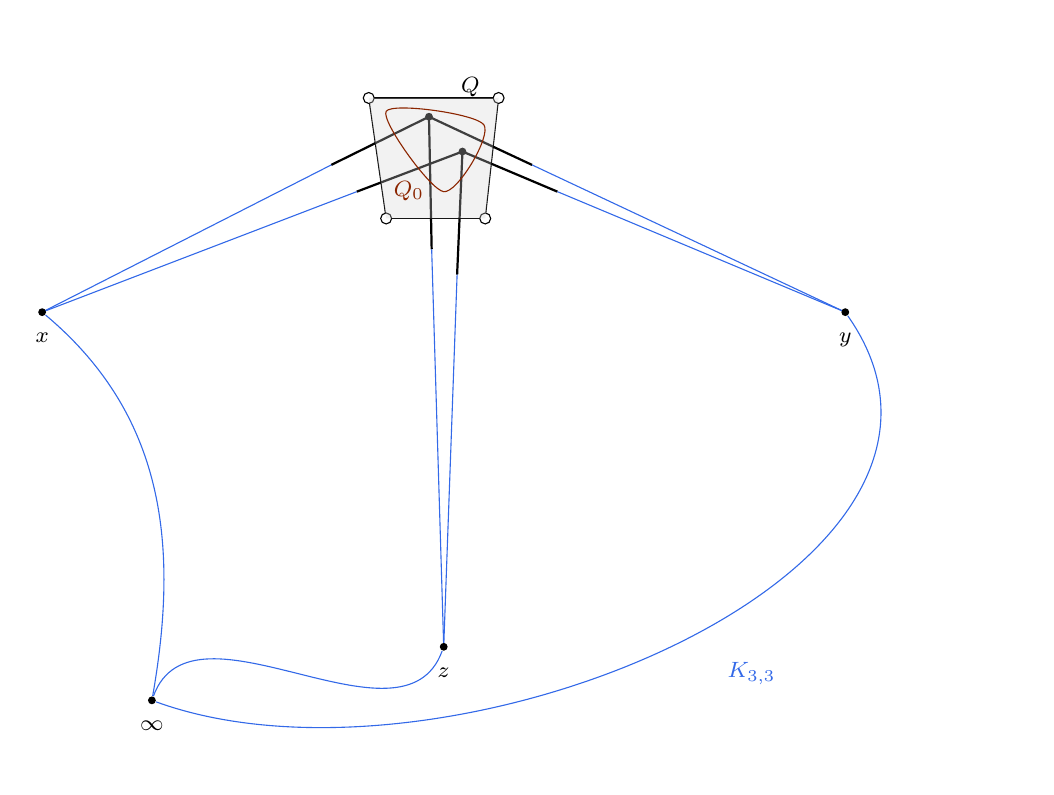
\begin{tikzpicture}[scale = 1.7, node distance=0.1cm,>=latex, dot/.style={circle,inner sep=1pt,fill,label={#1}, name=#1},
  extended line/.style={shorten >=-#1,shorten <=-#1},
 extended line/.default=1cm,
 dot2/.style={circle,inner sep=1.4pt,draw,fill=white,label={#1}, name=#1}]

\begin{footnotesize}
\draw [thick] (3.14,1.2)-- (3.1,0.28);
\draw [ thick] (2.89,1.46)-- (2.91,0.47);
\draw [ thick] (2.89,1.46)-- (3.66,1.1);
\draw [ thick] (3.14,1.2)-- (3.85,0.9);
\draw [ thick] (2.16,1.1)-- (2.89,1.46);
\draw [ thick] (2.35,0.9)-- (3.14,1.2);
\draw [] (2.44,1.6)-- (3.41,1.6);
\draw [] (3.41,1.6)-- (3.31,0.7);
\draw [] (3.31,0.7)-- (2.57,0.7);
\draw [] (2.57,0.7)-- (2.44,1.6);
\draw [color=blue] (2.35,0.9)-- (0,0);
\draw [color=blue] (2.16,1.1)-- (0,0);
\draw [color=blue] (3.1,0.28)-- (3,-2.5);
\draw [color=blue] (2.91,0.47)-- (3,-2.5);
\draw [color=blue] (3.85,0.9)-- (6,0);
\draw [color=blue] (3.66,1.1)-- (6,0);

%\draw [dotted] (2.35,2.4)-- (3,-2.5);
%\draw [dotted] (3.5,2.4)-- (3,-2.5);
%\draw [dotted] (0,0)-- (6,0);
%\draw [dotted] (0,0)-- (3,-2.5);
%\draw [dotted] (6,0)-- (3,-2.5);

\node [dot=](p1) at (2.89,1.46) {};
%\node [left = of p1] {$p_{1}$};

\node [dot=](p2) at (3.14,1.2) {};
%\node [left = of p2] {$p_{2}$};

\node [dot=](y) at (6,0) {};
\node [below = of y] {$y$};

\node [dot=](z) at (3,-2.5) {};
\node [below = of z] {$z$};

\node [dot=](x) at (0,0) {};
\node [below = of x] {$x$};

\node [dot=](inf) at (0.82,-2.9) {};
\node [below = of inf] {$\infty$};


\node [dot2=](t1) at (2.44,1.6) {};
\node [dot2=](t2) at (3.41,1.6) {};
\node [dot2=](t3) at (3.31,0.7) {};
\node [dot2=](t4) at (2.57,0.7) {};

\fill[color-trapezoid, opacity=0.3] (2.44,1.6) -- (3.41,1.6) -- (3.31,0.7) -- (2.57,0.7) --  (2.44,1.6) -- cycle;
%\draw [] (t1) -- (t2) -- (t3) -- (t4) -- (t1) -- cycle;

% draw the area T_0 inside T

\draw [red] plot [smooth cycle] coordinates {(2.57,1.5) (3.3,1.4) (3,0.9) };

\coordinate (t0) at (2.74, 1.1);
\node [red,below = of t0] {$Q_{0}$};

\coordinate (t) at (3.2,1.49);
\node [above = of t] {$Q$};

\coordinate (k33) at (5,-2.7);
\node [blue, right = of k33] {$K_{3,3}$};

\draw [blue]  (x) to[out=-40,in=80] (inf);
\draw [blue]  (y) to[out=-55,in=-20] (inf);
\draw [blue]  (z) to[out=-110,in=70] (inf);


\end{footnotesize}
\end{tikzpicture}

\caption{Drawing of $K_{3,3}$ can have crossing only in trapezoid $Q$.}
\label{fig: k33-trapezoid}
\end{figure}


\begin{theorem}[Trapezoid crossing]
\label{thm: k33-trapezoid}
Let $\Pi$ be the basis of the partial drawing of complete graph and $x,y,z \in \Pi$. Let $Q$ be $xyz$-ray trapezoid in $Q_{0} \subseteq Q$. If for any point in $Q_{0}$ holds that its $x, y, z$ stubs intersect legs and short base of the ray trapezoid $Q$, then for every two points $p_{1}, p_{2}$ from $Q_{0}$ holds
$$
Y_{p_{1},x,y,z} \cap Y_{p_{2},x,y,z} \neq \emptyset.
$$
\end{theorem}
\begin{proof}
Suppose we have in $Q_{0}$ two points $p_{1}$ and $p_{2}$ from the basis $\Pi$. Clearly  $x \not\in Q_{0}$ and consequently $x \neq p_{1}$ and $x \neq p_{2}$. Extend the stubs $\overline{p_{i}}x, \overline{p_{i}}y$ and $\overline{p_{i}}z$, for $i = 1,2$, to line segments $\overline{p_{i}x}, \overline{p_{i}y}$ and $\overline{p_{i}z}$. Choose any point $\infty$, which lies below the points $x,y,z$ and connect it with points $x,y,z$ without producing additional crossings, see Figure~\ref{fig: k33-trapezoid}. The result is a drawing of graph $K_{3, 3}$, which contains at least one intersection. Any intersection can only be contained in $Q$, therefore
$$
Y_{p_{1},x,y,z} \cap Y_{p_{2},x,y,z} \neq \emptyset.
$$
\end{proof}

The Theorem~\ref{thm: k33-trapezoid} will typically be used with the region $Q_{0} = Q$, or $Q_{0}$ will be ray trapezoid with the same left and right boundaries as $Q$. An analogous theorem about the region inside a triangle follows.


\begin{theorem}[Triangle crossing]
\label{thm: k33-triangle}
Let $\Pi$ be the basis of partial drawing of complete graph and $x,y,z \in \Pi$. Let the lines $p_{x}, p_{y}, p_{z}$ be parallel to line segments $\overline{yz}, \overline{xz}, \overline{xy}$. Suppose that for the region $T_{0} \subset T$ holds that for each point $p \in T_{0}$ its $x,y,z$-stubs $\overline{p}x, \overline{p}y, \overline{p}z$ intersect the sides of the triangle $T$, which lie on the lines $p_{x}, p_{y}, p_{z}$. Then for every two points $p_{1}, p_{2} \in T_{0}$ holds
$$
Y_{p_{1},x,y,z} \cap Y_{p_{2},x,y,z} \neq \emptyset.
$$
\end{theorem}

\begin{proof}
Suppose we have in $T_{0}$ two points $p_{1}, p_{2}$ from the basis $\Pi$.
Extend the stubs $\overline{p_{i}}x, \overline{p_{i}}y, \overline{p_{i}}z$, for $i = 1,2$, to lines $\overline{p_{i}x}, \overline{p_{i}y}, \overline{p_{i}z}$. Choose any point $\infty$ that lies below the points $x,y,z$ so that we do not produce additional crossings, see Figure~\ref{fig: k33-triangle}. Result is a drawing of $K_{3, 3}$, which contains at least one intersection. Any intersection can only be contained in $T$, therefore
$$
Y_{p_{1},x,y,z} \cap Y_{p_{2},x,y,z} \neq \emptyset.
$$
\end{proof}

\begin{figure}
\centering
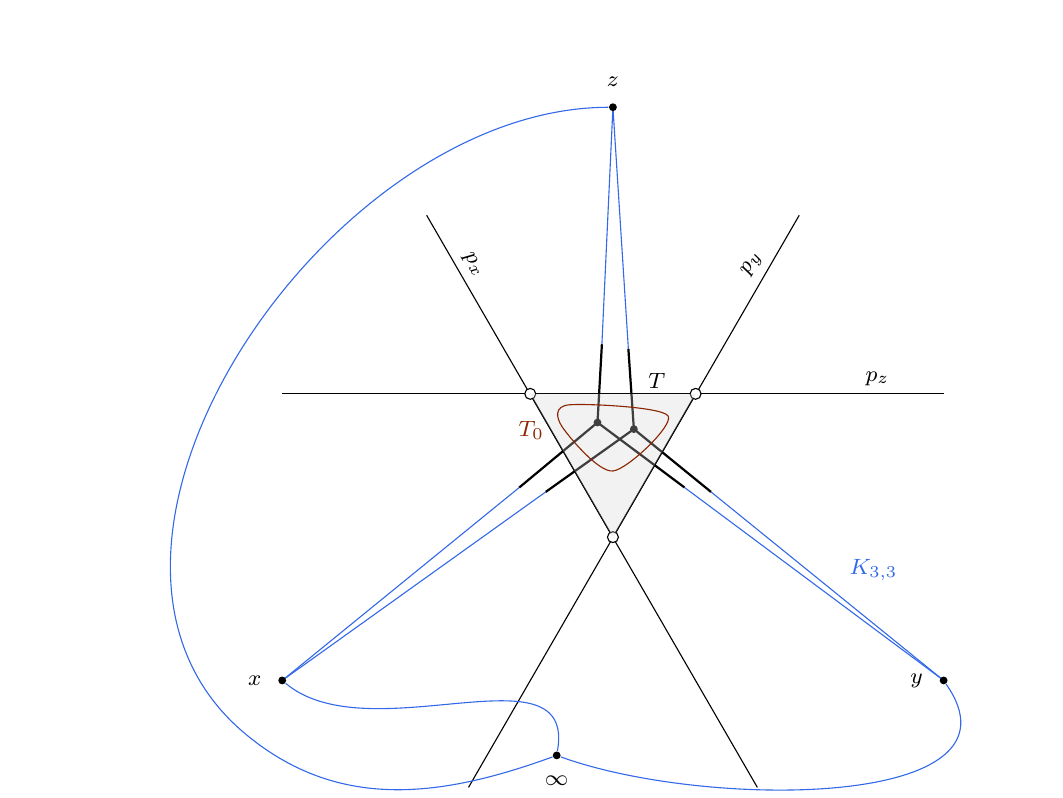
\begin{tikzpicture}[scale = 1.4, node distance=0.1cm,>=latex, dot/.style={circle,inner sep=1pt,fill,label={#1}, name=#1},
  extended line/.style={shorten >=-#1,shorten <=-#1},
 extended line/.default=1cm,
  dot2/.style={circle,inner sep=1.4pt,draw,fill=white,label={#1}, name=#1}]
\begin{footnotesize}

% analogous theorem about the region inside a triangle
\draw [thick](3.19,2.28)-- (3.14,3.01);
\draw [thick] (2.86,2.34)-- (2.9,3.05);
\draw [thick]  (2.86,2.34)-- (3.65,1.75);
\draw [thick] (3.19,2.28)-- (3.89,1.71);
\draw [thick] (2.15,1.75)-- (2.86,2.34);
\draw [thick] (2.39,1.71)-- (3.19,2.28);
\draw [blue] (2.39,1.71)-- (0,0);
\draw [blue] (2.15,1.75)-- (0,0);
\draw [blue] (3.14,3.01)-- (3,5.2);
\draw [blue] (2.9,3.05)-- (3,5.2);
\draw [blue] (3.89,1.71)-- (6,0);
\draw [blue] (3.65,1.75)-- (6,0);

\draw (1.31,4.22) -- (4.31,-0.97) node[pos=0.1,sloped,above] {$p_{x}$}; %px
\draw (0,2.6)-- (6,2.6) node[pos=0.9,sloped,above] {$p_{z}$}; %pz
\draw (4.69,4.22)-- (1.69,-0.97) node[pos=0.1,sloped,above] {$p_{y}$}; %py

\draw [] (2.25,2.6)-- (3,1.3);
\draw [] (3,1.3)-- (3.75,2.6);
\draw [] (3.75,2.6)-- (2.25,2.6);


\node [dot=](p1) at (2.86,2.34) {};
%\node [below = of p1] {$p_{1}$};

\node [dot=](p2) at (3.19,2.28) {};
%\node [below = of p2] {$p_{2}$};

\node [dot=](x) at (0,0) {};
\node [left = of x] {$x$};

\node [dot=](y) at (6,0) {};
\node [left = of y] {$y$};

\node [dot=](z) at (3,5.2) {};
\node [above = of z] {$z$};


\node [dot=](inf) at (2.49,-0.68) {};
\node [below = of inf] {$\infty$};

\node [dot2=](k) at (2.25,2.6) {};
\node [dot2=](l) at (3.75,2.6) {};
\node [dot2=](h) at (3,1.3) {};

\fill[color-inside, opacity=0.3] (2.25,2.6) -- (3.75,2.6) -- (3,1.3) -- (2.25,2.6) -- cycle;
%\draw [] (t1) -- (t2) -- (t3) -- (t4) -- (t1) -- cycle;

% draw the area T_0 inside T
\draw [red] plot [smooth cycle] coordinates {(2.54,2.3) (2.6,2.5) (3.5,2.4) (3,1.9)};

\coordinate (t0) at (2.26, 2.5);
\node [red,below = of t0] {$T_{0}$};

\coordinate (t) at (3.4,2.5);
\node [above = of t] {$T$};

\coordinate (k33) at (5,1);
\node [blue, right = of k33] {$K_{3,3}$};

\draw [blue]  (x) to[out=-40,in=80] (inf);
\draw [blue]  (y) to[out=-55,in=-20] (inf);
\draw [blue]  (z) to[out=180,in=140] (-0.34,-0.48);
\draw [blue]  (-0.34,-0.48) to[out=-40,in=200] (inf);

\end{footnotesize}
\end{tikzpicture}

\caption{Drawing of $K_{3,3}$ can have crossing only in triangle $T$.}
\label{fig: k33-triangle}
\end{figure}

For the ray trapezoid $Q$ corresponding to the Theorem~\ref{thm: k33-trapezoid}, we have shown
$$
m(Q) = 1.
$$
Also for the triangle $T$ corresponding to the Theorem~\ref{thm: k33-triangle}
$$
m(T) = 1
$$
holds.

\section{Transformation}
It will sometimes be advantageous to use geometric symmetry when estimating the maximum number of points of a partial drawing of a complete graph. For example, we would like to estimate the number of points from $\Pi$ in the triangle $\trisym{abc}$. If the triangle $\trisym{abc}$ is equilateral, we will use symmetry to our advantage. Typically, the triangle $\trisym{abc}$ will not be of this shape, but using the appropriate transformation we can convert it to equilateral. A plane transformation is \textit{affine} if it is a composite of linear transformation and parallel translation.

\begin{theorem}[Transformation]
\label{thm: transformation}
Let $\Phi$ be an invertible affine transformation of the plane. Then $\Pi$ is the basis of the partial drawing of the complete graph if and only if $\Phi(\Pi)$ is the basis of the partial drawing of the complete graph.
\end{theorem}

\begin{proof}
A partial drawing of a full graph is a union of lines. Invertible affine transformation of the plane maps disjoint line segments into disjoint line segments. However, if the line segments $\overline{ab}, \overline{ac}$ have a common vertex $a$ then their $\Phi$-images have a common edge $\Phi(a)$.
\end{proof}

Using the transformation theorem, we can assume that, for example, the triangle $\trisym{abc}$ is equilateral or the rectangle $\rectansym{ab}\abovesym{b}\abovesym{a}$ is a square, of course not both at the same time.

\chapter{Estimates}
For the basis of the partial drawing $\Pi$ we assume Properties~\ref{list: properties} and use the notation in accordance with the mentioned properties. We present the chosen division of frame, which depends on the position of the points $c$ and $d$. For the remainder of the chapter, for each region of frame division, we estimate the upper bound on the number of basis points that each region can contain. From the sum of the obtained estimates, we get the upper bound for the number of points of the basis of the partial drawing of the complete graph. Let’s write down our main result.

\begin{theorem}
The maximum possible number of points in the basis of a partial drawing of a complete graph is $101$. Symbolically, if $\Pi$ is the basis of a partial drawing, then
\begin{equation}
  |\Pi| \leq 101.
\end{equation}
\label{thm: main}
\end{theorem}


\section{Frame division}
\begin{figure}
\centering
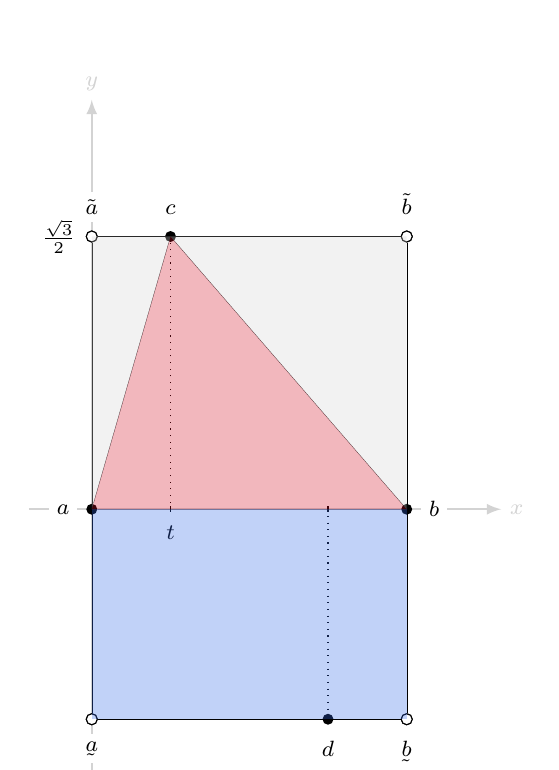
\begin{tikzpicture}[scale = 4, node distance=0.1cm,>=latex, dot/.style={circle,inner sep=1.4pt,fill,label={#1}, name=#1},
dot2/.style={circle,inner sep=1.4pt,draw,fill=white,label={#1}, name=#1}]
\begin{footnotesize}
% axes
\draw[gray,thick,->] ({-0.2}, 0) -- (1.3, 0) node[right] {$x$};
\draw[gray,thick,->] (0, {-2/3-0.2}) -- (0, 1.3) node[above] {$y$};
\node [dot=](a) at (0,0) {};
\node [dot=](b) at (1,0) {};
\node [dot=](c) at ({1/4},{sqrt(3)/2}) {};
\node [dot=](d) at ({3/4}, {-2/3}) {};
\node [dot2=](abovea) at (0,{sqrt(3)/2}) {};
\node [dot2=](aboveb) at (1,{sqrt(3)/2}) {};
\node [dot2=](undera) at (0,{-2/3}) {};
\node [dot2=](underb) at (1,{-2/3}) {};


% denote where c and d are
%%%%%%%%%%%%%% c
\draw [thin] (0.2500000000, 0.01000000000) -- (0.2500000000, -0.01000000000);
\coordinate (t) at (0.25,0);
\node [below = of t] {$t$}; % = \frac{1}{4}
\draw [thin] (-0.01, {sqrt(3)/2}) -- (0.01, {sqrt(3)/2});
\coordinate (cy) at (0,{sqrt(3)/2});
\node [left = of cy] {$\frac{\sqrt{3}}{2}$};
\draw[thin,dotted] (t) -- (c);
\draw[thin,dotted] (cy) -- (c);
%%%%%%%%%%%%%%%% d
\draw [thin] ({3/4}, 0.01000000000) -- ({3/4}, -0.01000000000);
\coordinate (dx) at ({3/4},0);
\draw [thin] (-0.01, {-2/3}) -- (0.01, {-2/3});
\coordinate (u) at (0,{-2/3});
%\node [left = of u] {$u = -\frac{1}{3}$};
\draw[thin,dotted] (u) -- (d);
\draw[thin,dotted] (dx) -- (d);
%[semithick,black]
\draw[ultra thin] (undera) -- (underb) -- (aboveb) -- (abovea) -- (undera) -- cycle;
\draw[ultra thin] (a) -- (b) -- (c) -- (a) -- cycle;
\node [right = of b,fill=white] {$b$};
\node [left = of a,fill=white] {$a$};
\node [above = of c] {$c$} {};
\node [below = of d] {$d$}; %fill=white
\node [dot2=](abovea) at (0,{sqrt(3)/2}) {};
\node [above = of abovea,fill=white] {$\abovesym{a}$};
\node [dot2=](aboveb) at (1,{sqrt(3)/2}) {};
\node [above = of aboveb] {$\abovesym{b}$};
\node [dot2=](undera) at (0,{-2/3}) {};
\node [below = of undera, fill=white] {$\undersym{a}$};
\node [dot2=](underb) at (1,{-2/3}) {};
\node [below = of underb] {$\undersym{b}$};
%\node [below = of dx,fill=white] {$\frac{2}{3}$};


\fill[orange, opacity=0.3] (0,0) -- (1,0) -- ({1/4},{sqrt(3)/2}) -- (0,0) -- cycle;
\fill[gray,opacity=0.3] (0,0) -- ({1/4},{sqrt(3)/2}) -- (0,{sqrt(3)/2}) -- (0,0) -- cycle;
\fill[gray,opacity=0.3] (1,0) -- ({1/4},{sqrt(3)/2}) -- (1,{sqrt(3)/2}) -- (1,0) -- cycle;
\fill[blue,opacity=0.3] (0,0) -- (1,0) -- (1,{-2/3}) -- (0,{-2/3}) -- (0,0) -- cycle;
\end{footnotesize}
\end{tikzpicture}

\caption{Division of the frame $F$ into a central, left, and right triangle, and a bottom triangle.}
\label{fig: frame-subsets}
\end{figure}

For an easier presentation, according to the Theorem~\ref{thm: transformation}(Transformation), we can stretch the basis $\Pi$ and thus the frame $F$ in the direction of $y$-coordinate. Thus we achieve that the $y$-coordinate of the point $c$ (this coordinate is denoted by $c_{y}$) will be equal to $\frac{\sqrt{3}}{2}$, see Figure~\ref{fig: frame-subsets}. This changes the distances between the points, and the distance between the mapped points $a$ and $b$ is no longer necessarily the largest. However, we do not change the non-crossing property of stubs. In the frame $F$, define the following polygons:

\begin{enumerate}
  \item[{1)}] \textit{central triangle} $\trisym{abc}$;
  \item[{3)}] \textit{left and right triangle} $\trisym{ac\abovesym{a}}$ in $\trisym{b\abovesym{b}c}$;
  \item[{3)}] \textit{lower quadrilateral} $\rectansym{\undersym{a}\undersym{b}ba}$.
\end{enumerate}

In Figure~\ref{fig: frame-subsets} is the division of the frame $F$, where $t = c_{x} = \frac{1}{4}$ and $d_{y} = -\frac{2}{3}$ (points $a$ and $b$ are at the maximum distance in $\Pi$).  Vertices of the frame $F$ are not part of the set $\Pi$, so they are drawn with white circles. All auxiliary points, which are not necessarily part of the set $\Pi$, will be drawn with white circles.

We will first make the estimate for the central triangle $\trisym{abc}$ absolute, and if $h$ is large enough (point $d$ is low enough), we will improve it. The estimates of the number of basis points in the left and right triangles will depend on the value of the parameter $t$. Our take on the estimate for the lower quadrilateral is by using the parameters $t = c_{x}$ in $h = -\frac{d_{y}}{c_{y}}$ simultaneously. We start with the central triangle $\trisym{abc}$.

\section{Central triangle}
In this section we estimate the upper bound for the number of basis points in the central triangle $|\Pi \cap \trisym{abc}|$. According to the Theorem~\ref{thm: transformation}(Transformation) we can assume that $\trisym{abc}$ is equilateral.

\begin{figure}
\begin{center}
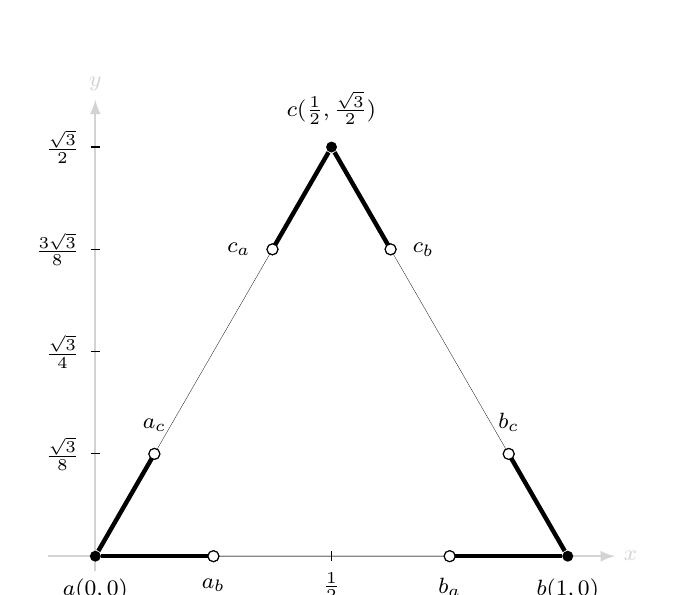
\begin{tikzpicture}[scale = 6, node distance=0.1cm,>=latex, dot/.style={circle,inner sep=1.4pt,fill,label={#1}, name=#1},
dot2/.style={circle,inner sep=1.4pt,draw,fill=white,label={#1}, name=#1}]
\begin{footnotesize}
% axes
\draw[gray,thick,->] ({-0.1}, 0) -- (1.1, 0) node[right] {$x$};
\draw[gray,thick,->] (0, {-0.1}) -- (0, {sqrt(3)/2 + .1}) node[above] {$y$};

% points
\node [dot=](a) at (0,0) {};
\node [below = of a,fill=white] {$a(0,0)$};
\node [dot=](b) at (1,0) {};
\node [below = of b] {$b(1,0)$};
\node [dot=](c) at ({1/2},{sqrt(3)/2}) {};
\node [above = of c] {$c(\frac{1}{2},\frac{\sqrt{3}}{2})$};

% stub ends
\node [dot2=](bc) at ({1 - 0.25*(0.5)}, {0.25*sqrt(3)/2}) {};
\node [above = of bc] {$b_{c}$};
\node [dot2=](cb) at ({1 - 0.75*(0.5)}, {0.75*sqrt(3)/2}) {};
\node [right = of cb] {$c_{b}$};

\node [dot2=](ac) at ({0.25*(0.5)}, {0.25*sqrt(3)/2}) {};
\node [above = of ac] {$a_{c}$};
\node [dot2=](ca) at ({0.75*(0.5)}, {0.75*sqrt(3)/2}) {};
\node [left = of ca] {$c_{a}$};

\node [dot2=](ab) at ({0.25},0) {};
\node [below = of ab] {$a_{b}$};
\node [dot2=](ba) at ({0.75}, 0)  {};
\node [below = of ba] {$b_{a}$};

%x,y,z
%\node [dot2=](x) at ({0.375}, {sqrt(3)/8}) {};
%\node [below = of x] {$x$};
%\node [dot2=](y) at ({0.625}, {sqrt(3)/8})  {};
%\node [below = of y] {$y$};
%\node [dot2=](z) at ({0.5}, {sqrt(3)/4})  {};
%\node [above = of z] {$z$};

%%%%%%%%%%%% to color it
%\fill[color-trapezoid, opacity=0.3] (a) -- ({0.25*(0.5)}, {0.25*sqrt(3)/2}) -- ({0.375}, {sqrt(3)/8}) -- ({0.25},0) -- (a) -- cycle;
%\fill[color-trapezoid, opacity=0.3] (b) -- ({1 - 0.25*(0.5)}, {0.25*sqrt(3)/2}) -- ({0.625}, {sqrt(3)/8}) -- ({0.75}, 0) -- (b) -- cycle;
%\fill[color-trapezoid, opacity=0.3] (c) -- ({1 - 0.75*(0.5)}, {0.75*sqrt(3)/2}) -- ({0.5}, {sqrt(3)/4}) -- ({0.75*(0.5)}, {0.75*sqrt(3)/2}) -- (c) -- cycle;
% color inside
%\fill[color-inside, opacity=0.3] ({0.375}, {sqrt(3)/8}) -- ({0.625}, {sqrt(3)/8}) -- ({0.5}, {sqrt(3)/4}) -- cycle;

% denote ticks 
% denote c and d
%%%%%%%%%%%%%% c
\draw [thin] (0.5, 0.01000000000) -- (0.5, -0.01000000000);
\coordinate (zx) at (0.5,0);
\node [below = of zx] {$\frac{1}{2}$}; % = 

\draw [thin] (-0.01, {sqrt(3)/8}) -- (0.01, {sqrt(3)/8});
\coordinate (xy) at (0,{sqrt(3)/8});
\node [left = of xy] {$\frac{\sqrt{3}}{8}$};

\draw [thin] (-0.01, {sqrt(3)/4}) -- (0.01, {sqrt(3)/4});
\coordinate (xz) at (0,{sqrt(3)/4});
\node [left = of xz] {$\frac{\sqrt{3}}{4}$};

\draw [thin] (-0.01, {3*sqrt(3)/8}) -- (0.01, {3*sqrt(3)/8});
\coordinate (kaza) at (0,{3*sqrt(3)/8});
\node [left = of kaza] {$\frac{3\sqrt{3}}{8}$};

\draw [thin] (-0.01, {sqrt(3)/2}) -- (0.01, {sqrt(3)/2});
\coordinate (cy) at (0,{sqrt(3)/2});
\node [left = of cy] {$\frac{\sqrt{3}}{2}$};

% big triangle
\draw[ultra thin] (a) -- (b) -- (c) -- (a) -- cycle;
% small triangle
%\draw[ultra thin] (x) -- (y) -- (z) -- (x) -- cycle;

% stubs
\draw[ultra thick] (b) -- ({1 - 0.25*(0.5)}, {0.25*sqrt(3)/2});
\draw[ultra thick] ({1 - 0.75*(0.5)}, {0.75*sqrt(3)/2}) -- (c);
\draw[ultra thick] (a) -- ({0.25*(0.5)}, {0.25*sqrt(3)/2});
\draw[ultra thick] ({0.75*(0.5)}, {0.75*sqrt(3)/2}) -- (c);
\draw[ultra thick] (a) -- ({0.25},0);
\draw[ultra thick] ({0.75}, 0) -- (b);

% parallelograms
%\draw[thin] (a) -- ({0.25*(0.5)}, {0.25*sqrt(3)/2}) -- ({0.375}, {sqrt(3)/8}) -- ({0.25},0) -- (a) -- cycle;
%\draw[thin] (b) -- ({1 - 0.25*(0.5)}, {0.25*sqrt(3)/2}) -- ({0.625}, {sqrt(3)/8}) -- ({0.75}, 0) -- (b) -- cycle;
%\draw[thin] (c) -- ({1 - 0.75*(0.5)}, {0.75*sqrt(3)/2}) -- ({0.5}, {sqrt(3)/4}) -- ({0.75*(0.5)}, {0.75*sqrt(3)/2}) -- (c) -- cycle;
%\draw [thin] (0,0) -- (1,0) -- ({1/2},{sqrt(3)/2}) -- cycle;


% again white circles to draw over the lines
\node [dot2=](bc) at ({1 - 0.25*(0.5)}, {0.25*sqrt(3)/2}) {};
\node [dot2=](cb) at ({1 - 0.75*(0.5)}, {0.75*sqrt(3)/2}) {};
\node [dot2=](ac) at ({0.25*(0.5)}, {0.25*sqrt(3)/2}) {};
\node [dot2=](ca) at ({0.75*(0.5)}, {0.75*sqrt(3)/2}) {};
\node [dot2=](ab) at ({0.25},0) {};
\node [dot2=](ba) at ({0.75}, 0)  {};
%\node [dot2=](x) at ({0.375}, {sqrt(3)/8}) {};
%\node [dot2=](y) at ({0.625}, {sqrt(3)/8})  {};
%\node [dot2=](z) at ({0.5}, {sqrt(3)/4})  {};
%\node [above = of z] {$z$};

\end{footnotesize}
\end{tikzpicture}

\end{center}
\caption{The central triangle can be transformed into an equilateral one.}
\label{fig: triangle-abc}
\end{figure}

For $u,v \in \left\{ {a,b,c} \right\}$, where $u \neq v$, we define the points $u_{v}$ as the ends of all stubs between the points $a,b, c$, see Figure~\ref{fig: triangle-abc}.

% inner triangle
The intersections of the lines $\overline{a_{b}c_{b}}$, $\overline{c_{a}b_{a}}$ and $\overline{a_{c}b_{c}}$ are denoted by $a',b',c'$ and with them we define \textit{inner triangle} $\trisym{a'b'c'}$, which is presented in Figure~\ref{fig: inner-triangle}. Using the central symmetry of the central triangle $\trisym{abc}$, we define two more groups of congruent polygons.

% corner regions
Intersection of lines $\overline{b_{c}a}$ and $\overline{b_{a}c}$ with coordinates $(\frac{7}{10},\frac{\sqrt{3}}{10})$ is denoted by $b^{*}$ and we define \textit{corner region} at $b$ as quadrilateral
$$
\quadsym{b_{a}bb_{c}b^{*}}.
$$
Symmetrically define the corner regions at $a$ and $c$:
$$
\quadsym{aa_{b}a^{*}a_{c}},
$$
$$
\quadsym{cc_{a}c^{*}c_{b}}.
$$
Corner regions are deltoids, because $\trisym{abc}$ is equilateral. They are presented in blue in Figure~\ref{fig: corner-regions}.

\begin{figure}
\begin{center}
\input{./tikz/subsets-of-triangle-abc.subfig}
\end{center}
\caption{Polygons in the central triangle.}
\label{fig: subsets-of-triangle-abc}
\end{figure}

% inner layers
We choose a ray coordinate system with respect to $a, b, c$. This means that the point $c$ is the origin, half-line from $c$ trough $a$ is the ray axis.

\textit{Inner layer} with respect to $a,b,c$ is a ray trapezoid:
$$
\tpz{\left[ \frac{1}{4},\frac{3}{4},\frac{3}{4},1 \right]_{a,b,c} }.
$$
The remaining two inner layers are determined by the same ray coordinates with respect to corresponding permutations of the points $a,b,c$:
$$
\tpz{\left[ \frac{1}{4},\frac{3}{4},\frac{3}{4},1 \right]_{a,c,b} },
$$
$$
\tpz{\left[ \frac{1}{4},\frac{3}{4},\frac{3}{4},1 \right]_{b,c,a} }.
$$
\textit{Inner layers} in Figure~\ref{fig: inner-layers} are shaded. We notice that they partially overlap.

\begin{figure}
\begin{center}
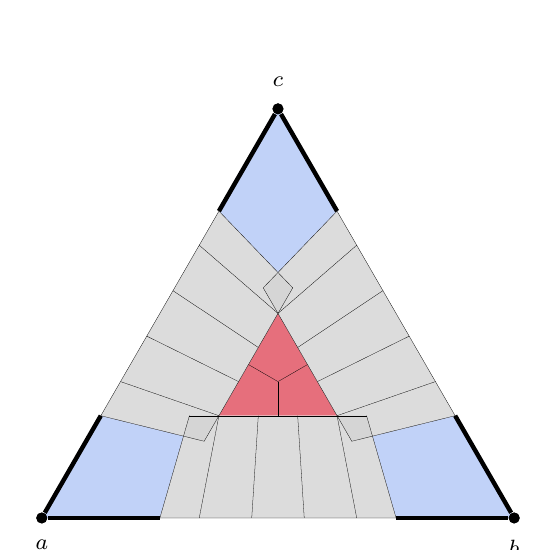
\begin{tikzpicture}[scale = 6, node distance=0.1cm,>=latex, dot/.style={circle,inner sep=1.4pt,fill,label={#1}, name=#1},
dot2/.style={circle,inner sep=1.4pt,draw,fill=white,label={#1}, name=#1}]
% axes
%\draw[gray,thick,->] ({-0.1}, 0) -- (1.1, 0) node[right] {$x$};
%\draw[gray,thick,->] (0, {-0.1}) -- (0, {sqrt(3)/2 + .1}) node[above] {$y$};

% color inside
\fill[orange,opacity=0.6] ({0.375}, {sqrt(3)/8}) -- ({0.625}, {sqrt(3)/8}) -- ({0.5}, {sqrt(3)/4}) -- cycle;

%% color deltoids
% deltoid_a
\fill[blue,opacity=0.3] (0,0) -- (0.25,0) -- (0.3, 0.173205) -- (0.125, 0.216506) -- (0,0) -- cycle;
% deltoid_b
\fill[blue,opacity=0.3] (0.75,0) -- (1,0) -- (0.875, 0.216506) -- (0.7, 0.173205) -- (0.75,0) -- cycle;
% deltoid_c
\fill[blue,opacity=0.3] (0.5, 0.866025) -- (0.625, 0.649519) -- (0.5, 0.519615) -- (0.375, 0.649519) -- (0.5, 0.866025) -- cycle;

% color trapezoids
\fill[gray,opacity=0.8] ({0.3125},{0.2165063509}) -- ({0.2500000000},{0}) -- ({0.7500000000},{0}) -- ({0.6875},{0.2165063509}) -- cycle;
\fill[gray,opacity=0.8] ({0.46875},{0.4871392896}) -- ({0.625},{0.6495190528}) -- ({0.875},{0.2165063509})-- ({0.65625},{0.1623797632}) -- cycle;
\fill[grey,opacity=0.8] ({0.53125},{0.4871392896}) -- ({0.375},{0.6495190528}) -- ({0.125},{0.2165063509}) -- ({0.34375},{0.1623797632}) -- cycle;


\node [dot=](a) at (0,0) {};
\node [dot=](b) at (1,0) {};
\node [dot=](c) at ({1/2},{sqrt(3)/2}) {};


\begin{footnotesize}
% points
\node [dot=](a) at (0,0) {};
\node [below = of a,fill=white] {$a$};
\node [dot=](b) at (1,0) {};
\node [below = of b] {$b$};
\node [dot=](c) at ({1/2},{sqrt(3)/2}) {};
\node [above = of c] {$c$};

% c
%\draw [thin] (0.5, 0.01000000000) -- (0.5, -0.01000000000);
%\coordinate (zx) at (0.5,0);
%\node [below = of zx] {$\frac{1}{2}$};
%
%\draw [thin] (-0.01, {sqrt(3)/8}) -- (0.01, {sqrt(3)/8});
%\coordinate (xy) at (0,{sqrt(3)/8});
%\node [left = of xy] {$\frac{\sqrt{3}}{8}$};
%
%\draw [thin] (-0.01, {sqrt(3)/4}) -- (0.01, {sqrt(3)/4});
%\coordinate (xz) at (0,{sqrt(3)/4});
%\node [left = of xz] {$\frac{\sqrt{3}}{4}$};
%
%\draw [thin] (-0.01, {3*sqrt(3)/8}) -- (0.01, {3*sqrt(3)/8});
%\coordinate (kaza) at (0,{3*sqrt(3)/8});
%\node [left = of kaza] {$\frac{3\sqrt{3}}{8}$};
%
%\draw [thin] (-0.01, {sqrt(3)/2}) -- (0.01, {sqrt(3)/2});
%\coordinate (cy) at (0,{sqrt(3)/2});
%\node [left = of cy] {$\frac{\sqrt{3}}{2}$};

%[semithick,black]
\draw[ultra thin] (a) -- (b) -- (c) -- (a) -- cycle;

% lines
% inner - deltoids
\draw [ultra thin] ({0.5}, {0.2165063509461096}) -- ({0.5}, {0.28867513459481287});
\draw [ultra thin] ({0.5625}, {0.3247595264191645}) -- ({0.5}, {0.28867513459481287});
\draw [ultra thin] ({0.4375}, {0.3247595264191645}) -- ({0.5}, {0.28867513459481287});

% draw stubs
\draw[ultra thick] (b) -- ({1 - 0.25*(0.5)}, {0.25*sqrt(3)/2});
\draw[ultra thick] ({1 - 0.75*(0.5)}, {0.75*sqrt(3)/2}) -- (c);
\draw[ultra thick] (a) -- ({0.25*(0.5)}, {0.25*sqrt(3)/2});
\draw[ultra thick] ({0.75*(0.5)}, {0.75*sqrt(3)/2}) -- (c);
\draw[ultra thick] (a) -- ({0.25},0);
\draw[ultra thick] ({0.75}, 0) -- (b);


% simmetrically inside
\draw [ultra thin] ({0.3125},{0.2165063509}) -- ({0.2500000000},{0});
\draw [ultra thin] ({0.375},{0.2165063509}) -- ({0.3333333333},{0});
\draw [ultra thin] ({0.458333},{0.2165063509}) -- ({0.4444444444},{0});
\draw [ultra thin] ({0.541667},{0.2165063509}) -- ({0.5555555556},{0});
\draw [ultra thin] ({0.625},{0.2165063509}) -- ({0.6666666667},{0});
\draw [ultra thin] ({0.6875},{0.2165063509}) -- ({0.7500000000},{0});
\draw [ultra thin] ({0.3125},{0.2165063509}) -- ({0.6875},{0.2165063509});

\draw [ultra thin] ({0.46875},{0.4871392896}) -- ({0.625},{0.6495190528});
\draw [ultra thin] ({0.5},{0.4330127019}) -- ({0.666667},{0.5773502692});
\draw [ultra thin] ({0.541667},{0.3608439182}) -- ({0.722222},{0.4811252243});
\draw [ultra thin] ({0.583333},{0.2886751346}) -- ({0.777778},{0.3849001795});
\draw [ultra thin] ({0.625},{0.2165063509}) -- ({0.833333},{0.2886751346});
\draw [ultra thin] ({0.65625},{0.1623797632}) -- ({0.875},{0.2165063509});
\draw [ultra thin] ({0.46875},{0.4871392896}) -- ({0.65625},{0.1623797632});

\draw [ultra thin] ({0.53125},{0.4871392896}) -- ({0.375},{0.6495190528});
\draw [ultra thin] ({0.5},{0.4330127019}) -- ({0.333333},{0.5773502692});
\draw [ultra thin] ({0.458333},{0.3608439182}) -- ({0.277778},{0.4811252243});
\draw [ultra thin] ({0.416667},{0.2886751346}) -- ({0.222222},{0.3849001795});
\draw [ultra thin] ({0.375},{0.2165063509}) -- ({0.166667},{0.2886751346});
\draw [ultra thin] ({0.34375},{0.1623797632}) -- ({0.125},{0.2165063509});
\draw [ultra thin] ({0.53125},{0.4871392896}) -- ({0.34375},{0.1623797632});

% stub ends
%\node [dot2=](bc) at ({1 - 0.25*(0.5)}, {0.25*sqrt(3)/2}) {};
%\node [above = of bc] {$b_{c}$};
%\node [dot2=](cb) at ({1 - 0.75*(0.5)}, {0.75*sqrt(3)/2}) {};
%\node [right = of cb] {$c_{b}$};
%
%\node [dot2=](ac) at ({0.25*(0.5)}, {0.25*sqrt(3)/2}) {};
%\node [above = of ac] {$a_{c}$};
%\node [dot2=](ca) at ({0.75*(0.5)}, {0.75*sqrt(3)/2}) {};
%\node [left = of ca] {$c_{a}$};
%
%\node [dot2=](ab) at ({0.25},0) {};
%\node [below = of ab] {$a_{b}$};
%\node [dot2=](ba) at ({0.75}, 0)  {};
%\node [below = of ba] {$b_{a}$};
\end{footnotesize}
\end{tikzpicture}

\end{center}
\caption{Coverage of central triangle $\trisym{abc}$.}
\label{fig: united-cover-abc}
\end{figure}

The inner triangle and both groups of congruent polygons form the coverage of the central triangle, see Figure~\ref{fig: united-cover-abc}. For each deltoid (see the same figure) in the inner triangle and for each cell in the inner layers, we will show that it contains at most one point of the partial drawing. For each corner area, we will show that it contains a maximum of $6$ points of partial drawing. The estimate for the number of points in the corner areas touching the points $a$ and $b$ will be improved by using the lowermost point $d$ in the lower quadrilateral $\quadsym{\undersym{a}\undersym{b}ba}$ of the frame $F$. Points $a,b,c$ are considered separately. We pretend that they do not belong to any area or cell, and their presence is taken into account only at the very end of the assessment.

The sum of the obtained estimates for the coverage regions of the central triangle $\trisym{abc}$ will give the estimate of the upper bound for the number of basis points in the central triangle, which will depend on the parameter $h$ (position of the point $d$). In the following, we reveal why we chose such a central triangle coverage and why the inner layers are not disjoint. In dealing with both groups of polygons, we describe and apply the ideas, which we later extend and apply to the remaining subsets of the frame $F$.

\subsection{Inner triangle}

\begin{figure}
\begin{center}
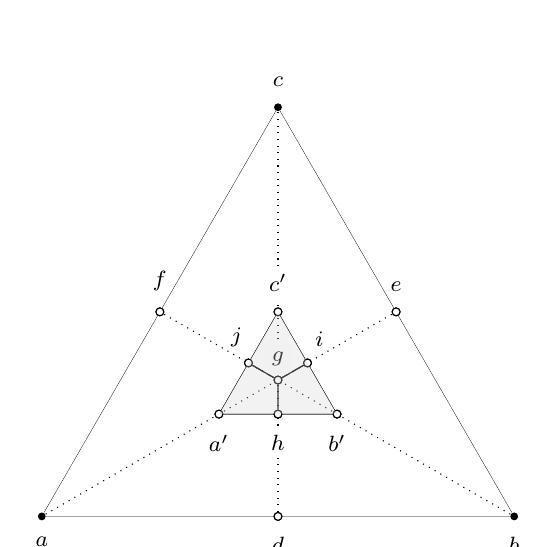
\begin{tikzpicture}[scale = 6, node distance=0.1cm,>=latex, dot/.style={circle,inner sep=1pt,fill,label={#1}, name=#1},
dot2/.style={circle,inner sep=1pt,draw,fill=white,label={#1}, name=#1}]
\begin{footnotesize}
% points
\node [dot=](a) at (0,0) {};
\node [below = of a,fill=white] {$a$};
\node [dot=](b) at (1,0) {};
\node [below = of b] {$b$};
\node [dot=](c) at ({1/2},{sqrt(3)/2}) {};
\node [above = of c] {$c$};

% x,y,z
\node [dot2=](x) at ({0.375}, {sqrt(3)/8}) {};
\node [below = of x] {$a'$};
\node [dot2=](y) at ({0.625}, {sqrt(3)/8})  {};
\node [below = of y] {$b'$};
\node [dot2=](z) at ({0.5}, {sqrt(3)/4})  {};
% d,e,f, g, h, i, j, k, l
\node [dot2=](d) at ({0.5}, 0) {};
\node [below = of d] {$d$};
\node [dot2=](e) at ({0.75}, {sqrt(3)/4})  {};
\node [above = of e] {$e$};
\node [dot2=](f) at ({0.25}, {sqrt(3)/4})  {};
\node [above = of f] {$f$};
\node [dot2=](g) at ({0.5}, {sqrt(3)/6})  {};
\node [dot2=](h) at ({1/2},{sqrt(3)/8})  {};

\node [dot2=](i) at ({1/2+1/16},{3*sqrt(3)/16})  {};
\coordinate (ifix) at ({1/2+1/16+0.025},{3*sqrt(3)/16});
\node [above = of ifix] {$i$};

\node [dot2=](j) at ({1/2-1/16},{3*sqrt(3)/16})  {};
\coordinate (jfix) at ({1/2-1/16-0.025},{3*sqrt(3)/16});
\node [above = of jfix] {$j$};

%\node [dot2=](k) at ({3/8},{sqrt(3)/4})  {};
%\node [above = of k] {$k$};
%\node [dot2=](l) at ({5/8},{sqrt(3)/4})  {};
%\node [above = of l] {$l$};
 

% big triangle 
\draw[ultra thin] (a) -- (b) -- (c) -- (a) -- cycle;
% inner small triangle
\draw[ultra thin] (x) -- (y) -- (z) -- (x) -- cycle;
% triangle median, deltoide, sigma'
\draw[ thin,dotted] (d) -- (c);
\draw[ thin,dotted] (a) -- (e);
\draw[ thin,dotted] (b) -- (f);
\draw[] (g) -- (h);
\draw[] (g) -- (i);
\draw[] (g) -- (j);
%\draw[thin, dotted] (h) -- (l) -- (k) -- (h) -- cycle;

% ticks of heights
% 2/3, 1/2, ... 
%\draw [thin] (0.2575000000, 0.4286825749) -- (0.2425000000, 0.4373428289);
%\node [left = of f] {$\frac{1}{2}$};
%\draw [thin, dotted] (f) -- (k);
%\draw [thin, dotted] (l) -- (e);
%
%\draw [thin] (0.1741666667,0.2843450076) -- (0.1591666667,0.2930052616);
%\draw [thin, dotted] (0.1666666667,0.2886751346) -- (0.8333333333,0.2886751346);

% again white points to cover the lines
\coordinate (gfix) at ({0.5}, {sqrt(3)/6-0.005});
\node [above = of gfix, fill=white] {$g$};
\draw[] (g) -- (i);
\draw[] (g) -- (j);
% inner small triangle
\draw[ultra thin] (x) -- (y) -- (z) -- (x) -- cycle;

\node [below = of h,fill=white] {$h$};
% x,y,z
\node [dot2=](x) at ({0.375}, {sqrt(3)/8}) {};
\node [dot2=](y) at ({0.625}, {sqrt(3)/8})  {};
\node [dot2=](z) at ({0.5}, {sqrt(3)/4})  {};
% d,e,f, g, h, i, j, k, l
\node [dot2=](d) at ({0.5}, 0) {};
\node [dot2=](e) at ({0.75}, {sqrt(3)/4})  {};
\node [dot2=](f) at ({0.25}, {sqrt(3)/4})  {};
\node [dot2=](g) at ({0.5}, {sqrt(3)/6})  {};
\node [dot2=](h) at ({1/2},{sqrt(3)/8})  {};
\node [dot2=](i) at ({1/2+1/16},{3*sqrt(3)/16})  {};
\node [dot2=](j) at ({1/2-1/16},{3*sqrt(3)/16})  {};
%\node [dot2=](k) at ({3/8},{sqrt(3)/4})  {};
%\node [dot2=](l) at ({5/8},{sqrt(3)/4})  {};
\node [above = of z,fill=white] {$c'$};

\fill[color-inside,opacity=0.3] ({0.375}, {sqrt(3)/8}) -- ({0.625}, {sqrt(3)/8}) -- ({0.5}, {sqrt(3)/4}) -- ({0.375}, {sqrt(3)/8}) -- cycle;

\end{footnotesize}
\end{tikzpicture}

\end{center}
\caption{Divide the inner triangle into three congruent deltoids.}
\label{fig: deltoids}
\end{figure}

In the central triangle $\trisym{abc}$ we denote the bisectors of the sides by $d, e, f$, and median with $g$, see Figure~\ref{fig: deltoids}. The point $g$ divides the median in the ratio $1:2$, so the $y$-coordinate of the point $g$ is equal to one third of the $y$-coordinate of the point $c$. The intersections of medians with the sides of the inner triangle $\trisym{a'b'c'}$ are denoted by $h, i, j$. Define the points that divide the inner triangle into three congruent deltoids:
$$
\quadsym{a'hgj},\text{\hspace{0.8cm}} \quadsym{hb'ig}\text{\hspace{0.8cm}   and   \hspace{0.8cm}} \quadsym{gic'j}.
$$

For them, we show that each contains at most one point from the set $\Pi$. From here we get the following estimate:

\begin{figure}
\begin{center}
\input{./tikz/deltoids-together.subfig}
\end{center}
\caption{For Proposition~\ref{prop: deltoids}.}
\label{fig: deltoids-together}
\end{figure}

\begin{proposition}
\label{prop: deltoids}
The inner triangle $\trisym{a'b'c'}$ contains a maximum of 3 basis points. Symbolically
$$
  m(\trisym{a'b'c'}) = 3.
$$
\end{proposition}

\begin{proof}
Denote one of the deltoids by $T_{0}$
$$
  \quadsym{a'hgj},\text{\hspace{0.8cm}} \quadsym{hb'ig}\text{\hspace{0.8cm}   and   \hspace{0.8cm}} \quadsym{gic'j}.
$$
The following property must be shown. If $p \in T_{0}$, then its stubs $\overline{p}a,\overline{p}b,\overline{p}c$ intersect all three sides of the triangle $T$ (for the shaded deltoid $T_{0}$ in Figures~\ref{fig: deltoids} is a triangle $T$ drawn in bold).

Let $x$ be any point from deltoid
$$
  \quadsym{gic'j}
$$
and $y$ any point from deltoid
$$
  \quadsym{hb'ig}.
$$
Because of symmetry, it suffices to show that the stub $\overline{x}c$ (Figure~\ref{fig: side-kl}) intersects the line segment $\overline{kl}$ and the stub $\overline{y}c$ (Figure~\ref{fig: side-jm}) intersects the line segment $\overline{jm}$.

Place the origin of ray coordinate system at the point $c$ and let the ray axis run from $c$ to $a$. The point $g$ is at the ray height $\frac{2}{3}$ from the point $c$, the points $a',h,b'$ are at the ray height $\frac{3}{4}$, points $k, c', l$ at $\frac{1}{2}$ and points $j,i,m$ at $\frac{5}{8}$.

The ray height of the point $x$ is on the interval
$$
  \left[\frac{1}{2}, \frac{2}{3}\right],
$$
and the ray height of the point $y$ on the interval
$$
  \left[\frac{5}{8}, \frac{3}{4}\right].
$$
Since
$$
  \frac{2}{3} \cdot \frac{3}{4} \leq \frac{1}{2}
$$
the stub $\overline{x}c$ intersects $\overline{kl}$ and since
$$
  \frac{3}{4} \cdot \frac{3}{4} \leq \frac{5}{8}
$$
the stub $\overline{y}c$ intersects $\overline{jm}$.

Theorem~\ref{thm: k33-triangle} using $T_{0} = \quadsym{gic'j}$ and $T = \trisym{hlk}$ claims that $|\Pi \cap T_{0}| \leq 1$. Therefore, using symmetry, the claim is proved.
\end{proof}

\subsection{Corner regions}
Let
$$
Q = \quadsym{b_{a}bb_{c}b^{*}},
$$
see Figure~\ref{fig: first-relationship}, and $p,p'$ any poins from $\left(\Pi \cap Q\right) \setminus \left\{ b \right\}$. Stubs $\overline{p}a$ and $\overline{p'}a$ intersect the line segment $\overline{b_{a}b^{*}}$ and stubs $\overline{p}c$ and $\overline{p'}c$ intersect the line segment $\overline{b_{c}b^{*}}$. Therefore, one of the angles $\sangle{apc}, \sangle{ap'c}$ is contained in the other. Without the loss of generality, it should apply

\begin{equation}
\label{eq: nesting-angles}
\sangle{apc} \subseteq \sangle{ap'c}.
\end{equation}

We say the points $p,p' \in \left(\Pi \cap Q\right) \setminus \left\{ b \right\}$ are \textit{nested}.

\begin{figure}
\begin{center}
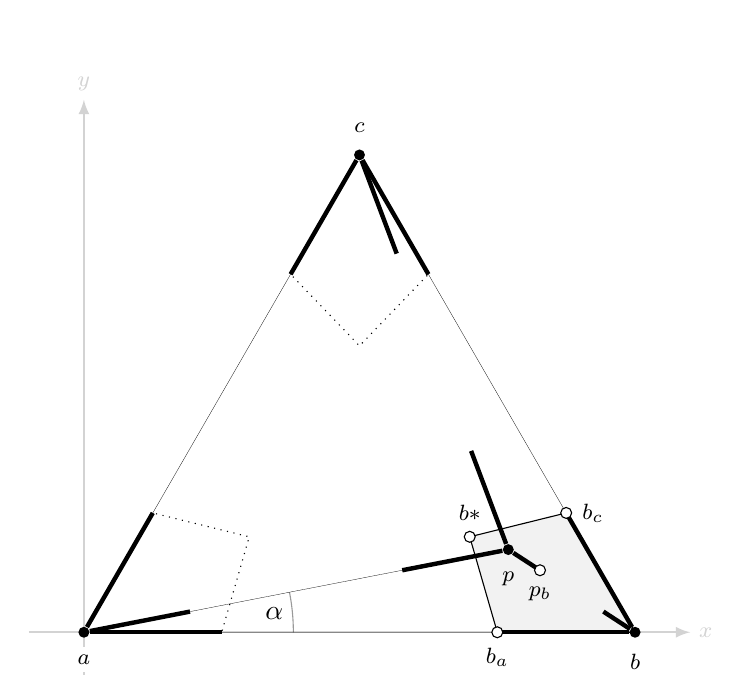
\begin{tikzpicture}[scale = 7, node distance=0.1cm,>=latex, dot/.style={circle,inner sep=1.4pt,fill,label={#1}, name=#1},
dot2/.style={circle,inner sep=1.4pt,draw,fill=white,label={#1}, name=#1}]
\begin{footnotesize}
% axes
\draw[gray,thick,->] ({-0.1}, 0) -- (1.1, 0) node[right] {$x$};
\draw[gray,thick,->] (0, {-0.1}) -- (0, {sqrt(3)/2 + .1}) node[above] {$y$};

\fill[color-parallelogram,opacity=0.3] (0.75,0) -- (1,0) -- (0.875, 0.216506) -- (0.7, 0.173205) -- (0.75,0) -- cycle;

%%%%%%%%%%%%%%%%%%%%%%%% tocke 
\node [dot=](a) at (0,0) {};
\node [below = of a,fill=white] {$a$};
\node [dot=](b) at (1,0) {};
\node [below = of b] {$b$};
\node [dot=](c) at ({1/2},{sqrt(3)/2}) {};
\node [above = of c] {$c$};

\node [dot=] (p) at (0.77,0.15) {};

% stubes between p and a
\draw [ultra thick] (p) -- (0.5775, 0.1125) {};
\draw [ultra thick] (a) -- (0.1925, 0.0375) {};

% stubs between p and b
\draw [ultra thick] (p) -- (0.8275, 0.1125) {};
\draw [ultra thick] (b) -- (0.9425, 0.0375) {};

% stubs between p and c
\draw [ultra thick] (c) -- (0.5675, 0.687019) {};
\draw [ultra thick] (p) -- (0.7025, 0.329006) {};


% stub ends
\coordinate (pb) at (0.8275, 0.1125) {};
\node [below = of pb] {$p_{b}$};

\draw [ultra thin] (p) -- (a) {};

\coordinate (ba) at (0.75,0) {};
\node [below = of ba] {$b_{a}$};
\coordinate (bc) at (0.875,0.216506351) {};
\node [right = of bc] {$b_{c}$};

% b*, a*, c*
\coordinate (bzv) at (0.7, {sqrt(3)/10}) {};
\node [above = of bzv] {$b*$};

% deltoids
% deltoid_a
\draw[dotted] (0,0) -- (0.25,0) -- (0.3, 0.173205) -- (0.125, 0.216506) -- (0,0) -- cycle;
% deltoid_b
\draw[] (0.75,0) -- (1,0) -- (0.875, 0.216506) -- (0.7, 0.173205) -- (0.75,0) -- cycle;

% deltoid_c
\draw[dotted] (0.5, 0.866025) -- (0.625, 0.649519) -- (0.5, 0.519615) -- (0.375, 0.649519) -- (0.5, 0.866025) -- cycle;

% angles
\tkzMarkAngle[mark=none, size=0.38cm, opacity=.4](b,a,p)
\tkzLabelAngle[pos = 0.34](b,a,p){$\alpha$}

%\tkzMarkAngle[draw,size=0.56cm,%
%opacity=.4](pb,a,p)

%\tkzLabelAngle[pos = 0.54](pb,a,p){$\hat{\alpha}$}
%\draw [thin] (a) -- (pb);
% big triangle 
\draw[ultra thin] (a) -- (b) -- (c) -- (a) -- cycle;
% stubs
\draw[ultra thick] (b) -- ({1 - 0.25*(0.5)}, {0.25*sqrt(3)/2});
\draw[ultra  thick] ({1 - 0.75*(0.5)}, {0.75*sqrt(3)/2}) -- (c);
\draw[ultra  thick] (a) -- ({0.25*(0.5)}, {0.25*sqrt(3)/2});
\draw[ultra  thick] ({0.75*(0.5)}, {0.75*sqrt(3)/2}) -- (c);
\draw[ultra  thick] (a) -- ({0.25},0);
\draw[ultra  thick] ({0.75}, 0) -- (b);

% again white circles to cover the lines 
\node [dot2=] (bzv) at (0.7, {sqrt(3)/10}) {};
\node [dot2=] (ba) at (0.75,0) {};
\node [dot2=] (bc) at (0.875,0.216506351) {};
\node [dot2=] (pb) at (0.8275, 0.1125){};
\node [below = of p] {$p$};

\end{footnotesize}
\end{tikzpicture}


\end{center}
\caption{For Proposition~\ref{prop: nesting}}
% corner region is quadrilateral $Q$.
\label{fig: first-relationship}
\end{figure}

Denote $\alpha = \sangle{pab}$ and $\alpha' = \sangle{p'ab}$. Since the end $p_{b}$ of the stub $\overline{p}b$ lies inside the angle $\sangle{ap'c}$, the relationship
$$
\alpha \geq \frac{4}{3} \cdot \alpha',
$$
holds, since the angle $\sangle{pap_{b}} \geq \frac{1}{4}\alpha$, because $\sangle{apb} \geq \frac{\pi}{2}$. We summarize the statement using the above labels.

\begin{proposition} % about nesting
\label{prop: nesting}
Let $p,p' \in  \left(\Pi \cap Q\right) \setminus \left\{ b \right\}$. Angles $\sangle{apc}$ and $\sangle{ap'c}$ are comparable, and if
$$\sangle{apc} \subseteq \sangle{ap'c},$$
then the estimate
$$
  \alpha \geq \frac{4}{3} \cdot \alpha'.
$$
holds.
\end{proposition}

We will need another estimate. Since the pointers $\overline{p'}c$ and $\overline{p'}a$ do not intersect the line segment $\overline{bb_{p}}$, see Figure~\ref{fig: second-relationship}, for point $p'$ at least one of the inequalities holds
$$
  \sangle{p'ab} > \sangle{b_{p}ab}
$$
or
$$
  \sangle{p'cb} > \sangle{b_{p}cb}.
$$
Without the loss of generality let the first inequality hold
$$
  \alpha' > \sangle{b_{p}ab}.
$$
We can estimate the angle $\sangle{b_{p}ab}$ using trigonometry. Using the above notation, we can write a proposition.

\begin{figure}
\begin{center}
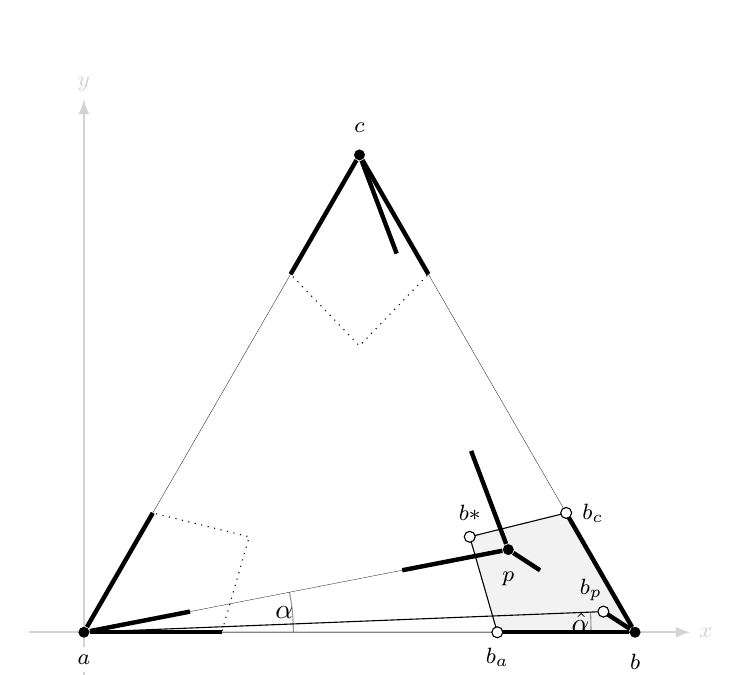
\begin{tikzpicture}[scale = 7, node distance=0.1cm,>=latex, dot/.style={circle,inner sep=1.4pt,fill,label={#1}, name=#1},
dot2/.style={circle,inner sep=1.4pt,draw,fill=white,label={#1}, name=#1}]
\begin{footnotesize}
% axes
\draw[gray,thick,->] ({-0.1}, 0) -- (1.1, 0) node[right] {$x$};
\draw[gray,thick,->] (0, {-0.1}) -- (0, {sqrt(3)/2 + .1}) node[above] {$y$};

\fill[color-parallelogram,opacity=0.3] (0.75,0) -- (1,0) -- (0.875, 0.216506) -- (0.7, 0.173205) -- (0.75,0) -- cycle;

% points
\node [dot=](a) at (0,0) {};
\node [below = of a,fill=white] {$a$};
\node [dot=](b) at (1,0) {};
\node [below = of b] {$b$};
\node [dot=](c) at ({1/2},{sqrt(3)/2}) {};
\node [above = of c] {$c$};

\node [dot=] (p) at (0.77,0.15) {};

% stubs between p and a
\draw [ultra thick] (p) -- (0.5775, 0.1125) {};
\draw [ultra thick] (a) -- (0.1925, 0.0375) {};

% stubs between p and b
\draw [ultra thick] (p) -- (0.8275, 0.1125) {};
\draw [ultra thick] (b) -- (0.9425, 0.0375) {};

% stubs between p and c
\draw [ultra thick] (c) -- (0.5675, 0.687019) {};
\draw [ultra thick] (p) -- (0.7025, 0.329006) {};


% stub ends
\coordinate (bp) at (0.9425, 0.0375) {};
%\node [above = of bp] {$b_{p}$};
\coordinate (kapaa) at (0.92, 0.028);
\node [above = of kapaa] {$b_{p}$};

\draw [ultra thin] (p) -- (a) {};

\coordinate (ba) at (0.75,0) {};
\node [below = of ba] {$b_{a}$};
\coordinate (bc) at (0.875,0.216506351) {};
\node [right = of bc] {$b_{c}$};

% b*, a*, c*
\coordinate (bzv) at (0.7, {sqrt(3)/10}) {};
\node [above = of bzv] {$b*$};

% deltoids
% deltoid_a
\draw[dotted] (0,0) -- (0.25,0) -- (0.3, 0.173205) -- (0.125, 0.216506) -- (0,0) -- cycle;
% deltoid_b
\draw[] (0.75,0) -- (1,0) -- (0.875, 0.216506) -- (0.7, 0.173205) -- (0.75,0) -- cycle;

% deltoid_c
\draw[dotted] (0.5, 0.866025) -- (0.625, 0.649519) -- (0.5, 0.519615) -- (0.375, 0.649519) -- (0.5, 0.866025) -- cycle;

% angles
\tkzMarkAngle[mark=none, size=0.38cm, opacity=.4](b,a,p)
\tkzLabelAngle[pos = 0.358](b,a,p){$\alpha$}

\tkzMarkAngle[mark=none, size=0.92cm, opacity=.4](b,a,bp)
\tkzLabelAngle[pos = 0.9](b,a,bp){$\hat{\alpha}$}

\draw [thin] (a) -- (bp);
% big triangle
\draw[ultra thin] (a) -- (b) -- (c) -- (a) -- cycle;
% stubs
\draw[ultra thick] (b) -- ({1 - 0.25*(0.5)}, {0.25*sqrt(3)/2});
\draw[ultra  thick] ({1 - 0.75*(0.5)}, {0.75*sqrt(3)/2}) -- (c);
\draw[ultra  thick] (a) -- ({0.25*(0.5)}, {0.25*sqrt(3)/2});
\draw[ultra  thick] ({0.75*(0.5)}, {0.75*sqrt(3)/2}) -- (c);
\draw[ultra  thick] (a) -- ({0.25},0);
\draw[ultra  thick] ({0.75}, 0) -- (b);


% again white circles to cover the lines 
\node [dot2=] (bzv) at (0.7, {sqrt(3)/10}) {};
\node [dot2=] (ba) at (0.75,0) {};
\node [dot2=] (bc) at (0.875,0.216506351) {};
\node [dot2=] (bp) at (0.9425, 0.0375) {};
\node [below = of p] {$p$};

\end{footnotesize}
\end{tikzpicture}


\end{center}
\caption{For Proposition~\ref{prop: stub-bpk}}
\label{fig: second-relationship}
\end{figure}

\begin{proposition}
\label{prop: stub-bpk}
Let $p,p' \in  \left(\Pi \cap Q\right) \setminus \left\{ b \right\}$, and assume that they are nested~\eqref{eq: nesting-angles} and
$$
  \alpha' > \sangle{b_{p}ab}.
$$

Then it applies
$$
  \alpha' > \frac{7}{37} \cdot \alpha.
$$
\end{proposition}

\begin{proof}
Denote $\hat{\alpha} = \sangle{b_{p}ab}$. Estimate the quotient $\frac{\alpha'}{\alpha}$. Since the tangent to $\left(0, \frac{\pi}{2}\right)$ is a convex and increasing function, it holds
\begin{equation*}
  \frac{\alpha'}{\alpha} \geq \frac{\tan(\alpha')}{\tan(\alpha)} \geq \frac{\tan(\hat{\alpha})}{\tan(\alpha)} = 1 - \frac{3}{3 + p_{x}},
\end{equation*}
where $p_{x}$ is the $x$-coordinate of the point $p$. The latter is bounded downwards by the $x$-coordinate of the point $b^{*}$, which is equal to $\frac{7}{10}$. That is why
\begin{equation*}
  \frac{\alpha'}{\alpha} > 1 - \frac{3}{3 + \frac{7}{10}} = \frac{7}{37}
\end{equation*}
and proposition holds.
\end{proof}

Using both propositions, we will be able to estimate the maximum possible number of points of the basis $\Pi$ in the quadrilateral $Q$. Let $\left\{ p_{1}, p_{2},...,p_{k} \right\}$ be the maximum set of points in $\left(\Pi \cap Q\right) \setminus \left\{ b \right\}$. According to Proposition~\ref{prop: nesting} we can assume without the loss of generality
$$
  \sangle{ap_{k}c} \subseteq \sangle{ap_{k-1}c} \subseteq ... \subseteq \sangle{ap_{2}c} \subseteq \sangle{ap_{1}c}
$$
and by Proposition~\ref{prop: stub-bpk} we can assume
$$
  \sangle{b_{p_{k}}ab} \leq \sangle{p_{1}ab}.
$$
Define the angles $\alpha_{i} = \sangle{bap_{i}}$, for $i = 1,..,k$. They are subject to relationships
\begin{equation}
\label{eq: sequence-alphas-1}
\alpha_{i} \geq \frac{4}{3} \cdot \alpha_{i-1} \text{,\hspace{0.8cm}   for    \hspace{0.8cm}} i = 2,...,k
\end{equation}

and

\begin{equation}
\label{eq: sequence-alphas-2}
\frac{\alpha_{1}}{\alpha_{k}} > \frac{7}{37}.
\end{equation}
By induction on above relationships, we produce an estimate
$$
\alpha_{1} \geq \frac{7}{37}  \cdot  \alpha_{k} \geq \frac{7}{37}  \cdot  \left(\frac{3}{4}\right)^{k-1}  \cdot \alpha_{1},
$$
which holds for $k \leq 6$. The following statement follows.
\begin{proposition}
\label{prop: corner-regions-1}
If $\Pi$ is the basis of a partial drawing and $Q = \quadsym{b_{a}bb_{c}b^{*}}$, then
\begin{equation}
\left|\left(\Pi \cap Q\right) \setminus \left\{ b \right\}\right| \leq 6.
\end{equation}
\end{proposition}

% improvement by taking into account point d
\begin{figure}
\begin{center}
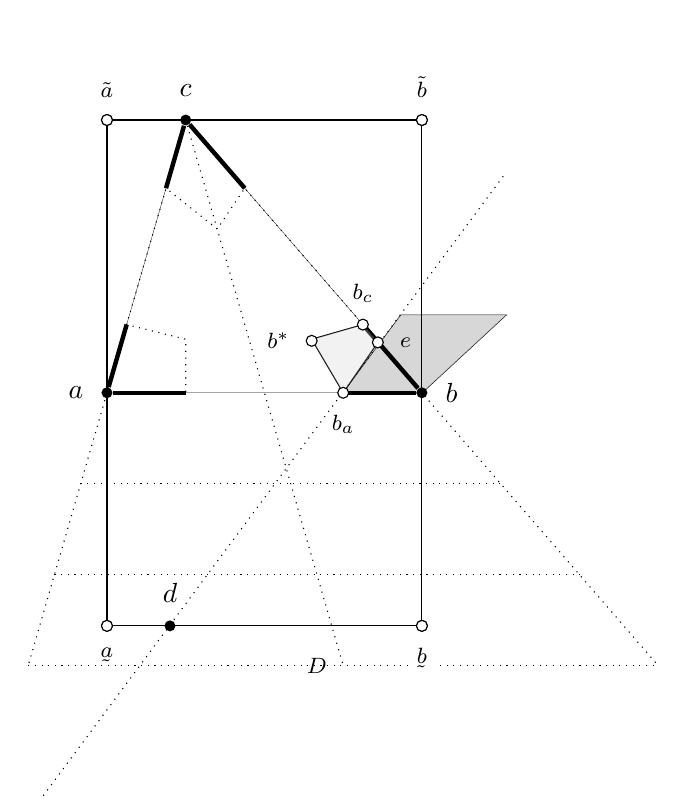
\begin{tikzpicture}[scale = 4, node distance=0.1cm,>=latex, dot/.style={circle,inner sep=1.4pt,fill,label={#1}, name=#1},
dot2/.style={circle,inner sep=1.4pt,draw,fill=white,label={#1}, name=#1}]

% shadow S_ba
\draw ({0.75}, 0) -- (1,0) -- (1.26667, 0.246667)  -- (.933333, 0.246667) -- (0.75,0) -- cycle;
\fill[color-parallelogram,opacity=0.9] ({0.75}, 0) -- (1,0) -- (1.26667, 0.246667)  -- (.933333, 0.246667) -- (0.75,0) -- cycle;

\node [dot=](a) at (0,0) {};
\node [left = of a] {$a$} {};
\node [dot=](b) at (1,0) {};
\node [right = of b] {$b$} {};
\node [dot=](c) at ({0.25},{sqrt(3)/2}) {};
\node [above = of c] {$c$} {};
\node [dot=](d) at (0.2,-0.74) {};
\node [above = of d] {$d$};

% axes
\draw[dotted] (c) -- (-0.25, -0.866025);
\draw[dotted] (c) -- (1.75, -0.866025);
\draw[dotted] (-0.25, -0.866025) -- (1.75, -0.866025);
\draw[dotted] (-0.0833333, -0.288675) -- (1.25, -0.288675);
\draw[dotted] (-0.166667, -0.57735) -- (1.5, -0.57735);
\draw[dotted] (c) -- (0.75, -0.866025);
\draw[dotted] (-0.24, -1.33) -- (1.26,0.69);
%\draw[dotted] (1.77,-0.35) -- (-0.66,0.76);;

 
\begin{footnotesize}
%\draw[color=black] (0,{sqrt(3)/2}) circle (inner sep=1pt);
\node [dot2=](abovea) at (0,{sqrt(3)/2}) {};
\node [dot2=](aboveb) at (1,{sqrt(3)/2}) {};
\node [dot2=](undera) at (0,-0.74) {};
\node [dot2=](underb) at (1,-0.74) {};

% frame F
\draw[] (undera) -- (underb) -- (aboveb) -- (abovea) -- (undera) -- cycle;
\draw[ultra thin] (a) -- (b) -- (c) -- (a) -- cycle;

% stubs
\draw[ultra thick] (b) -- (0.8125,0.216506);
\draw[ultra thick] (0.4375,0.649519) -- (c);

\draw[ultra thick] (a) -- (0.0625,0.216506);
\draw[ultra thick] (0.1875,0.649519) -- (c);

\draw[ultra thick] (a) -- ({0.25},0);
\draw[ultra thick] ({0.75}, 0) -- (b);

% color region for point d
%\fill[color-trapezoid,opacity=0.3] (0,{-2/3*sqrt(3)/2}) -- (0,{-sqrt(3)/2}) -- (0.75, -0.866025) -- (0.666667, -0.57735) -- (0,{-2/3*sqrt(3)/2}) -- cycle;
% -0.416667, -1.44338
% -0.25, -0.866025
%\fill[color-trapezoid,opacity=0.3] (-0.166667, -0.57735) -- (-0.25, -0.866025) -- (0.75, -0.866025) -- (0.666667, -0.57735) -- (-0.166667, -0.57735) -- cycle;

% color allowed area Q i.e. no shadow corners at b
\draw (0.75,0) -- (0.86,0.16) -- (0.8125,0.216506) -- (0.65,0.17) -- (0.75,0) -- cycle;
\fill[color-parallelogram,opacity=0.3] (0.75,0) -- (0.86,0.16) -- (0.8125,0.216506) -- (0.65,0.17) -- (0.75,0) -- cycle;
% dotted remaining corners
\draw[dotted] (0,0) -- (0.25,0) -- (0.25,0.17) -- (0.0625,0.216506) -- (0,0) -- cycle;
\draw[dotted] ({0.25},{sqrt(3)/2}) -- (0.4375,0.649519) -- (0.35,0.52) -- (0.1875,0.649519) -- ({0.25},{sqrt(3)/2}) -- cycle;

\node [dot2=](abovea) at (0,{sqrt(3)/2}) {};
\node [above = of abovea] {$\abovesym{a}$}; 

\node [dot2=](aboveb) at (1,{sqrt(3)/2}) {};
\node [above = of aboveb] {$\abovesym{b}$};

\node [dot2=](undera) at (0,-0.74) {};
\node [dot2=](underb) at (1,-0.74) {};

\node [below = of undera] {$\undersym{a}$};
\node [below = of underb,fill=white] {$\undersym{b}$};

\node [dot2=](ba) at (0.75,0) {};
\node [below = of ba] {$b_{a}$}; 
\node [dot2=](bc) at (0.8125,0.216506){};
\node [above = of bc] {$b_{c}$}; 
\node [dot2=](e) at (0.86,0.16){};
\node [right = of e] {$e$}; 
\node [dot2=](bstar) at (0.65,0.165){};
\node [left = of bstar] {$b^{*}$}; 
\coordinate (D) at (0.75, -0.866025) {};
\node [left = of D] {$D$}; 

\end{footnotesize}
\end{tikzpicture}

\end{center}
\caption{The shadow $S_{\overline{b}a}$ in ray coordinate system with respect to $a,b,d$ is represented as a dark gray area.}
\label{fig: corner-regions-improvement-1}
\end{figure}

The estimate of the number of basis points in the corner regions at $a$ and $b$ can be improved by assuming that the edge point $d$ is \textit{low enough} in the lower quadrilateral of the partial drawing. For the case when the parameter $h = -\frac{d_{y}}{c_{y}}$ it holds
$$
h \leq \frac{2}{3},
$$
see Figure~\ref{fig: corner-regions-improvement-1}. If the point $p \in \Pi \cap \trisym{abc}$ lies too close to the points $a$ or $b$, its stub $\overline{p}d$ intersects one of the stubs $\overline{a}b$ or $\overline{b}a$. The shadows
$$
S_{\overline{a}b} = \tpz{\left[ 0,\frac{1}{4},1,\frac{4}{3} \right]_{a,b,d}}
$$
and
$$
S_{\overline{b}a} = \tpz{\left[ \frac{3}{4},1,1,\frac{4}{3} \right]_{a,b,d}}
$$
depend on the position of the point $d$. We would like to improve the estimate in Proposition~\ref{prop: corner-regions-1} that follows from Proposition~\ref{prop: stub-bpk}, for the number of points in corner region $Q = \quadsym{bb_{a}b^{*}b_{c}}$ and consequently also in the region $\quadsym{aa_{b}a^{*}a_{c}}$. We do the following:

Using transformation, the triangle $\trisym{abc}$ is mapped into equilateral triangle. We show that the shadow of the pointer $\overline{b}a$ with respect to $d$ is minimal in a precisely determined position of the point $d$. In this position, we estimate the maximum number of basis points in $\quadsym{bb_{a}b^{*}b_{c}}$. The same estimate will apply to $quadsym{aa_{b}a^{*}a_{c}}$. The shadow $S_{\overline{b}a}$ is ray trapezoid in RCS with respect to $a, b, d$. The height of its long base is the smallest in the case when $h = \frac{2}{3}$ and its leg lies at a minimum angle exactly when the point $d$ lies on the extreme left border of the frame. In the case when $\trisym{abc}$ is equilateral (the frame is a parallelogram), the intersection $S_{\overline{b}a} \cap \trisym{abc}$ is minimal at the value of parameter $t = 0$, see Figure~\ref{fig: improvement-3}. Again, we denote by $k$ the maximum number of basis points 
$$
p_{1}, p_{2}, ..., p_{k}
$$
located in
$$
\left(\Pi \cap \quadsym{bb_{a}b^{*}b_{c}}\right) \setminus \left\{ b \right\},
$$
The points must not lie in the shadow of $S_{\overline{b}a}$ and we assume nesting property.

\begin{proposition}
The quadrilateral $\quadsym{bb_{a}b^{*}b_{c}} \setminus \left\{ b \right\}$ in the case of $h \geq \frac{2}{3}$ contains a maximum of $4$ basis points,
$$
|\left(\Pi \cap \quadsym{bb_{a}b^{*}b_{c}}\right) \setminus \left\{ b \right\}| \leq 4.
$$
\end{proposition}

\begin{proof}
The point at the intersection of the bisector of the angle $\sangle{abc}$ and the shadow side $\overline{b_{a}e}$ has coordinates at most $(\frac{22}{25},\frac{\sqrt{3}}{25})$ and denote it by $p^{*}$, see Figure~\ref{fig: improvement-3}. It holds
$$
\sangle{p^{*}ab} = \sangle{p^{*}cb} = \arctan{\frac{\sqrt{3}}{22}}.
$$

For point $p_{1}$ holds
$$
\sangle{p_{1}ab} \geq \sangle{p^{*}ab}
$$
or
$$
\sangle{p_{1}cb} \geq \sangle{p^{*}ab}.
$$
Without the loss of generality, we decide for the first case. Consequentially
$$
\alpha_{1} = \sangle{p_{1}ab} \geq \arctan{\frac{\sqrt{3}}{22}}.
$$
For the point $p_{k}$ holds the inequality
$$
\alpha_{k} = \sangle{p_{k}ab} \leq \arctan{\frac{\sqrt{3}}{7}}.
$$

If we also consider the nesting relationships~\ref{prop: nesting}
$$
\alpha_{i} \geq \frac{4}{3} \cdot \alpha_{i-1} \text{,\hspace{0.8cm}   for   \hspace{0.8cm}} i = 2,...,k,
$$
we produce the inequalities
$$
\arctan{\frac{\sqrt{3}}{7}} \geq \alpha_{k} \geq \left(\frac{4}{3}\right)^{k-1} \cdot \alpha_{1} \geq \left(\frac{4}{3}\right)^{k-1} \cdot \arctan{\frac{\sqrt{3}}{22}},
$$
which is fulfilled only at $k \leq 4$.
\end{proof}

\begin{figure}
\begin{center}
\begin{tikzpicture}[scale = 4, node distance=0.1cm,>=latex, dot/.style={circle,inner sep=1.4pt,fill,label={#1}, name=#1},
dot2/.style={circle,inner sep=1.4pt,draw,fill=white,label={#1}, name=#1}]

% axes
\draw[gray,thick,->] ({-0.6}, 0) -- (1.6, 0) node[right] {$x$};
\draw[gray,thick,->] (0, {-sqrt(3)/2-0.1}) -- (0, {sqrt(3)/2 + .1}) node[above] {$y$};

\node [right = of b,fill=white] {$b$};

% shadow S_ba
\draw ({0.75}, 0) -- (1,0) -- (1.44333, 0.193333)  -- (1.11, 0.193333) -- (0.75,0) -- cycle;
\fill[color-parallelogram,opacity=0.9] ({0.75}, 0) -- (1,0) -- (1.44333, 0.193333)  -- (1.11, 0.193333) -- (0.75,0) -- cycle;


%\fill[color-trapezoid,opacity=0.3] ({-1/2},{-sqrt(3)/2}) -- (0.5, -0.866025) -- (0.5, -0.57735) -- (-0.33, -0.58) -- ({-1/2},{-sqrt(3)/2}) -- cycle;

% deltoid_a
\draw[dotted] (0,0) -- (0.25,0) -- (0.3, 0.173205) -- (0.125, 0.216506) -- (0,0) -- cycle;
% deltoid_b
\draw[] (0.75,0) -- (0.94,0.1) -- (0.875, 0.216506) -- (0.7, 0.173205) -- (0.75,0) -- cycle;
\fill[color-parallelogram,opacity=0.3] (0.75,0) -- (0.94,0.1) -- (0.875, 0.216506) -- (0.7, 0.173205) -- (0.75,0) -- cycle;
% deltoid_c
\draw[dotted]  (0.5, 0.866025) -- (0.625, 0.649519) -- (0.5, 0.519615) -- (0.375, 0.649519) -- (0.5, 0.866025) -- cycle;

\begin{footnotesize}
\node [dot=](a) at (0,0) {};
\node [dot=](b) at (1,0) {};
\node [dot=](c) at ({1/2},{sqrt(3)/2}) {};
\node [above = of c] {$\abovesym{a} = c$};
\node [dot=](d) at (-0.33, -0.58) {};

\node [dot2=](overa) at ({1/2},{sqrt(3)/2}) {};
%\node [above = of overa] {$\abovesym{a}$};
\node [dot2=](overb) at ({3/2},{sqrt(3)/2}) {};
\node [above = of overb] {$\abovesym{b}$};
\node [dot2=](underb) at (0.666667, -0.57735) {};

% frame F
\draw[] (-0.33, -0.58) -- (underb) -- (overb) -- (overa) -- (-0.33, -0.58) -- cycle;
\draw[thin,dotted] (a) -- (b) -- (c) -- (a) -- cycle;

%% big triangle
\draw [thin,dotted] ({-1/2},{-sqrt(3)/2}) -- ({1/2},{sqrt(3)/2}) -- ({3/2},{-sqrt(3)/2}) -- cycle;

%% the lower two lines and the upper four tilted lines
\draw [thin,dotted]({-1/3},{-sqrt(3)/3}) -- ({4/3},{-sqrt(3)/3});
\draw [thin,dotted]({-1/6},{-sqrt(3)/6}) -- ({7/6},{-sqrt(3)/6});

% halves of 3/4 outwards
\draw [thin,dotted] (c) -- ({1/2},{-sqrt(3)/2});

% lines, e, p*, b*, corner regions
\draw [dotted] (-.66,.96) -- (1.8,-0.46);
%\draw [dotted] (-0.93,-0.9) -- (1.8,0.55);
\draw [dotted] (-0.93,-0.9) -- (1.8,0.557);

% stubs
\draw[ultra thick] (b) -- ({1 - 0.25*(0.5)}, {0.25*sqrt(3)/2});
\draw[ultra thick] ({1 - 0.75*(0.5)}, {0.75*sqrt(3)/2}) -- (c);
\draw[ultra thick] (a) -- ({0.25*(0.5)}, {0.25*sqrt(3)/2});
\draw[ultra thick] ({0.75*(0.5)}, {0.75*sqrt(3)/2}) -- (c);
\draw[ultra thick] (a) -- ({0.25},0);
\draw[ultra thick] ({0.75}, 0) -- (b);


\node [dot2=](e) at (0.94,0.1) {};
\node [right = of e] {$e$}; 
\node [dot2=](bzvezd) at (0.7, 0.173205) {};
\node [left = of bzvezd] {$b*$}; 
\node [dot2=](pzvezd) at (0.88,0.07) {};
\node [left = of pzvezd] {$p*$}; 

\node [dot2=](ba) at (0.75,0) {};
\node [below = of ba] {$b_{a}$}; 
\node [dot2=](bc) at (0.875, 0.216506) {};
\node [above = of bc] {$b_{c}$}; 
%\node [below = of undera] {$\undersym{a}$};
\node [below = of underb,fill=white] {$\undersym{b}$};
\node [left = of a,fill=white] {$a$};
\node [above = of d,fill=white] {$\undersym{a} = d*$};

% again the dots to cover the lines
\node [dot2=](overa) at ({1/2},{sqrt(3)/2}) {};
%\node [above = of overa] {$\abovesym{a}$};
\node [dot2=](overb) at ({3/2},{sqrt(3)/2}) {};
\node [above = of overb] {$\abovesym{b}$};
\node [dot2=](underb) at (0.666667, -0.57735) {};

\coordinate (D) at (0.5, -0.866025) {};
\node [left = of D] {$D$};

\end{footnotesize}
\end{tikzpicture}

\end{center}
\caption{The intersection $S_{\overline{b}a} \cap \trisym{abc}$ is minimal for the value of parameter $t = 0$.}
\label{fig: improvement-3}
\end{figure}

The section can be concluded with a cumulative estimate for the maximum number of basis points in the union of corner regions.

\begin{proposition}
\label{prop: corner-regions-union}
In the corner regions, if we exclude the points $a,b,c$, there is at most 18 basis points. However, if $h \geq \frac{2}{3}$ and we exclude the points $a,b,c$, there is at most 14 basis points. Symbolically
$$
\left|\left(\Pi \cap \left(
\quadsym{aa_{b}a^{*}a_{c}} \cup
\quadsym{bb_{a}b^{*}b_{c}} \cup
\quadsym{cc_{a}c^{*}c_{b}}
\right)\right)
\setminus \left\{ a,b,c \right\}\right| \leq \twopartdef
{ 14, } {h \geq \frac{2}{3},}
{ 18, } {h < \frac{2}{3}.}
$$
\end{proposition}

\subsection{Inner layers}
To estimate the number of basis points in the inner layers, by symmetry it is sufficient to consider one of them.

\begin{proposition}
\label{prop: inner-layer}
The inner belt contains a maximum of 5 basis points. Symbolically
$$
\left|
\tpz{\left[ \frac{1}{4},\frac{3}{4},\frac{3}{4},1 \right]_{a,b,c} } \cap \Pi
\right| \leq 5.
$$
\end{proposition}

\begin{proof}
We break the layer into 5 cells $C_{i}, i = 1,...,5$. Let $\beta_{i}, i = 0,...,5$ be cell boundaries. Cell $C_{i}$ has a left boundary $\beta_{i-1}$ and right boundary $\beta_{i}$. Cells are constructed starting from the left. The first four cells will be the largest, but the fifth cell will not:
\begin{align*}
\beta_{0} &= \frac{1}{4}, \\[6pt]%
\beta_{1} &= \min\left\{ f_{1,1}\left(\frac{1}{4}\right), f_{2,1}\left(\frac{1}{4}\right) \right\} = \frac{1}{3} \approx 0{,}33\text{\hspace{0.1cm}},\\[6pt]%
\beta_{2} &= \min\left\{ f_{1,1}\left(\frac{1}{3}\right), f_{2,1}\left(\frac{1}{3}\right) \right\} = \frac{4}{9} \approx 0{,}44\text{\hspace{0.1cm}},\\[6pt]%
\beta_{3} &= \min\left\{ f_{1,1}\left(\frac{4}{9}\right), f_{2,1}\left(\frac{4}{9}\right) \right\} = \frac{7}{12} \approx 0{,}58\text{\hspace{0.1cm}},\\[6pt]%
\beta_{4} &= \min\left\{ f_{1,1}\left(\frac{7}{12}\right), f_{2,1}\left(\frac{7}{12}\right) \right\} = \frac{11}{16} \approx 0{,}69\text{\hspace{0.2cm} and}\\[6pt]%
\beta_{5} &= \frac{3}{4}.
\end{align*}
Finally, it should be shown, that for each cell $C_{i},i=1,...,5$ holds
$$
m(C_{i}) = 1.
$$
Here we use the Theorem~\ref{thm: k33-trapezoid} (Trapezoid crossing) with $Q = C_{i}$ and $Q_{0} = C_{i}$. Choose any point $p \in C_{i}$. By definition, $\overline{p}z$ intersects the short base of trapezoid $C_{i}$. We need to check that the stubs $\overline{p}x, \overline{p}y$ intersect the legs of trapezoid $C_{i}$. The ray height of the point $p$ is denoted by
$$
\xi \in \left[\frac{3}{4}, 1 \right].
$$
The ray heights of the ends of the stubs $\overline{p}x, \overline{p}y$ are
$$
\frac{1+3\xi}{4} \in \left[\frac{3}{4}, 1 \right].
$$
Since the stub $\overline{p}x$ intersects $\beta_{i-1}$-ray and the stub $\overline{p}y$ intersects $\beta_{i}$-ray, the proposition is proved.
\end{proof}

We conclude the section with a cumulative estimate for the maximum number of basis points in the union of inner layers.

\begin{proposition}
\label{prop: inner-layers}
In the inner layers, there is a maximum of 15 basis points in total. Symbolically
$$
\left|
\Pi \cap \left(
\tpz{\left[ \frac{1}{4},\frac{3}{4},\frac{3}{4},1 \right]_{a,b,c} } \cup
\tpz{\left[ \frac{1}{4},\frac{3}{4},\frac{3}{4},1 \right]_{a,c,b} } \cup
\tpz{\left[ \frac{1}{4},\frac{3}{4},\frac{3}{4},1 \right]_{b,c,a} }
\right)
\right|
\leq 15.
$$
\end{proposition}

We summarize all the estimates in the inner triangle into a theorem:
\begin{theorem}
In the inner triangle $\trisym{abc}$, if we exclude the points $a,b,c$, there are at most 36 basis points. If $h \geq \frac{2}{3}$ and we exclude the points $a,b,c$, there are at most 32 basis points in the inner triangle. Symbolically
$$
\left|\left(\Pi \cap \trisym{abc}\right) \setminus \left\{ a,b,c \right\}\right| \leq \twopartdef
{ 32, } {h \geq \frac{2}{3},}
{ 36, } {h < \frac{2}{3}.}
$$
\end{theorem}
\begin{proof}
Use Proposition~\ref{prop: deltoids}, Proposition~\ref{prop: corner-regions-union} and Proposition~\ref{prop: inner-layers}.
\end{proof}

\section{Left and right triangle}
The left triangle $\trisym{ac\abovesym{a}}$ and the right triangle $\trisym{b\abovesym{b}c}$ depend on the parameter $t$, which represents the $x$-coordinate of the point $c$. Select the fixed $t$. We can observe only the left triangle $\trisym{ac\abovesym{a}}$ for each value of parameter $t$ from the interval $(0, 1)$. The corresponding drawing for the right triangle is obtained by mirroring the space over the vertical of the line segment $\overline{ab}$ for the parameter $1 - t$.

Let's transform the space so that the central triangle $\trisym{abc}$ becomes equilateral, see Figure~\ref{fig: upper-layers}. After the transformation, the point $c$ is fixed and the parameter $t$ represents the distance between the vertex $\abovesym{a}$ and the point $c$. The ray height of the vertex $\abovesym{a}$ is equal to $1 + t$. We choose a ray coordinate system according to the points $a,c,b$, so we place the origin at the point $b$ and the ray axis runs from $b$ to $a$.

\begin{figure}
\begin{center}
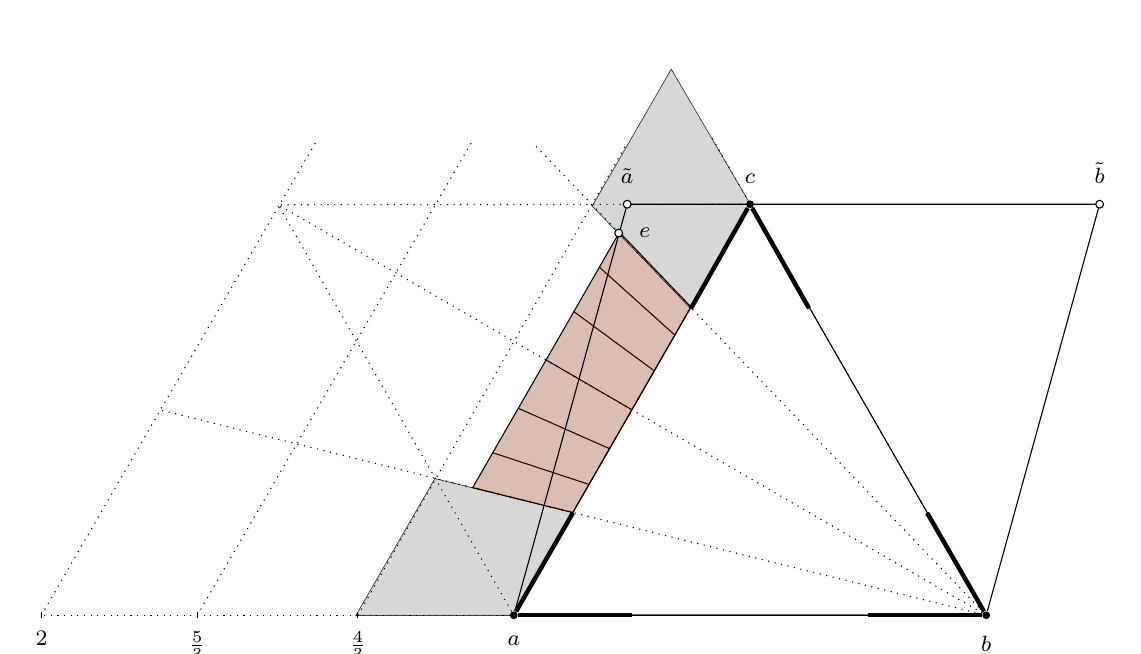
\begin{tikzpicture}[scale = 6, node distance=0.1cm,>=latex, dot/.style={circle,inner sep=1pt,fill,label={#1}, name=#1},
dot2/.style={circle,inner sep=1pt,draw,fill=white,label={#1}, name=#1}]

\begin{footnotesize}
\draw (0,0) -- (0.125, 0.216506) -- (-0.166667, 0.288675) -- (-0.333333, 0.) -- (0,0) -- cycle;
\fill[color-parallelogram,opacity=0.9] (0,0) -- (0.125, 0.216506) -- (-0.166667, 0.288675) -- (-0.333333, 0.) -- (0,0) -- cycle;

%% S_{ca}
\draw (0.375, 0.649519) -- (0.5,0.87) -- (0.333333, 1.1547) -- (0.166667, 0.866025) -- (0.375, 0.649519) -- cycle;
\fill[color-parallelogram,opacity=0.9] (0.375, 0.649519) -- (0.5,0.87) -- (0.333333, 1.1547) -- (0.166667, 0.866025) -- (0.375, 0.649519) -- cycle;

\node [dot=](a) at (0,0) {};
\node [below = of a] {$a$};
\node [dot=](b) at (1,0) {};
\node [below = of b] {$b$};
\node [dot=](c) at (0.5,0.87) {};
\node [above = of c] {$c$};
%
\draw [thin] ({0.375},{0.6525}) -- ({0.223602},{0.810559});
\draw [thin] ({0.340833},{0.59305}) -- ({0.181159},{0.736708});
\draw [thin] ({0.297328},{0.51735}) -- ({0.127115},{0.642671});
\draw [thin] ({0.25},{0.435}) -- ({0.068323},{0.540373});
\draw [thin] ({0.202672},{0.35265}) -- ({0.00953071},{0.438074});
\draw [thin] ({0.159167},{0.27695}) -- ({-0.0445135},{0.344037});
\draw [thin] ({0.125},{0.2175}) -- ({-0.0869565},{0.270186});
\draw [thin] ({0.375},{0.6525}) -- ({0.125},{0.2175});

\draw [thin] ({-0.0869565},{0.270186}) -- ({0.223602},{0.810559});
\fill[red,opacity=0.3] ({0.375},{0.6525}) -- ({0.125},{0.2175}) -- ({-0.0869565},{0.270186}) -- ({0.223602},{0.810559}) -- cycle;

\coordinate[]  (aa) at (0.24,0.87) {};
\coordinate[]  (bb) at (1.24,0.87) {};

\coordinate[]  (b12) at (-0.4987,0.869) {};
\coordinate[]  (b14b14) at (-0.75,0.435) {};
\coordinate[]  (b34b34) at (0.04,1) {};
\coordinate[]  (a2) at (-1,0) {};
\coordinate[]  (ac) at (0.13,0.22) {};
\coordinate[]  (ca) at (0.38,0.65) {};
\coordinate[]  (a43) at (-0.33,0) {};
\coordinate[]  (a43a43) at (0.24,1) {};
\coordinate[]  (a53) at (-0.67,0) {};

\coordinate[]  (e) at (0.23,0.8) {};
\coordinate[]  (a53a53) at (-0.09,1) {};
\coordinate[]  (a2a2) at (-0.42,1) {};
\coordinate[]  (o) at (0.42,1.01) {};

\draw[ultra thick] (b) -- ({1 - 0.25*(0.5)}, {0.25*sqrt(3)/2});
\draw[ultra thick] ({1 - 0.75*(0.5)}, {0.75*sqrt(3)/2}) -- (c);
\draw[ultra thick] (a) -- ({0.25*(0.5)}, {0.25*sqrt(3)/2});
\draw[ultra thick] ({0.75*(0.5)}, {0.75*sqrt(3)/2}) -- (c);
\draw[ultra thick] (a) -- ({0.25},0);
\draw[ultra thick] ({0.75}, 0) -- (b);

\draw [thin] (a) -- (b) -- (c) -- (a) -- cycle;
\draw [thin] (a) -- (b) -- (bb) -- (aa) -- (a) -- cycle;
\draw [dotted] (a) -- (b12) -- (c) -- cycle;

\draw [dotted] (b) -- (a2);
\draw [dotted] (b) -- (b14b14);
\draw [dotted] (b) -- (b12);
\draw [dotted] (b) -- (b34b34);
\draw [dotted] (b) -- (o);

\draw [dotted] (a43) -- (a43a43);
\draw [dotted] (a53) -- (a53a53);
\draw [dotted] (a2) -- (a2a2);

\draw [thin] (-0.33,0.00666173) -- (-0.33,-0.00666173); 
\node [below = of a43] {$\frac{4}{3}$};

\draw [thin] (-0.67,0.00666173) -- (-0.67,-0.00666173); 
\node [below = of a53] {$\frac{5}{3}$};

\draw [thin] (-1,0.00666173) -- (-1,-0.00666173); 
\node [below = of a2] {$2$};

\node [dot2=] (aa) at (0.24,0.87) {};
\node [above = of aa] {$\abovesym{a}$};
\node [dot2=] (bb) at (1.24,0.87) {};
\node [above = of bb] {$\abovesym{b}$};

\node [dot2=] (e) at (0.222,0.809) {};
\node [right = of e] {$e$};

\end{footnotesize}
\end{tikzpicture}
\end{center}
\caption{First upper layer for $t = 0.24.$}
\label{fig: upper-layers}
\end{figure}

For each value of parameter $t$ in the shadows $S_{\overline{a}c}$ and $S_{\overline{c}a}$ there will be no basis points except for the points $a$ and $c$. The maximum ray height of a point in the left triangle $\trisym{ac\abovesym{a}}$ that does not lie inside the shadow $S_{\overline{c}a}$ (it may lie on the edge of the shadow) is denoted by $\delta_{max}$. In Figure~\ref{fig: upper-layers} we marked the point $e$ with the maximum ray height $\delta_{max}$ with value of parameter $t = 0.24$.

The region in the left triangle without the shadows $S_{\overline{a}c}, S_{\overline{c}a}$ is covered by a maximum of three layers $L_{1},L_{2},L_{3}$. We define them as ray trapezoids with respect to $a, c, b$:
$$
L_{1} = \tpz{\left[ \alpha_{1},\omega_{1},\gamma_{1},\delta_{1} \right]_{a,c,b} },
$$
$$
L_{2} = \tpz{\left[ \alpha_{2},\omega_{2},\gamma_{2},\delta_{2} \right]_{a,c,b} },
$$
$$
L_{3} = \tpz{\left[ \alpha_{3},\omega_{3},\gamma_{3},\delta_{3} \right]_{a,c,b} }.
$$

The boundaries $\alpha_{i},\omega_{i},\gamma_{i},\delta_{i}, i = 1,2,3$, for each layer, depend on the value of parameter $t$ and are represented in Table~\ref{tab: upper-bounds-boundaries}. The table shows the following. If $t \leq \frac{1}{3}$ then $\delta_{max} \leq \frac{4}{3}$ and we say that the layers $L_{2}$ and $L_{3}$ are empty. The layer $L_{1}$ is always non-empty because $t > 0$ is always valid and therefore $\delta_{max} > 1$. For $t < \frac{1}{3}$, we adjust the upper ray height of the layer $L_{1}$ so that it is equal to $\delta_{max}$. The layer $L_{2}$ is not empty for $t > \frac{1}{3}$. For $t < \frac{2}{3}$, we adjust the upper ray height of the layer $L_{2}$ so that it is equal to $\delta_{max}$. The layer $L_{3}$ is not empty for $t > \frac{2}{3}$ and we adjust the upper ray height of this layer so that it is equal to $\delta_{max}$.

\begin{table*}
\centering
\begin{tabular}{@{}ccccccccc@{}}\toprule
& \multicolumn{1}{c}{$t \in [0,\frac{1}{3}]$} & \phantom{abc}& \multicolumn{2}{c}{$t \in (\frac{1}{3},\frac{2}{3}]$} &
\phantom{abc} & \multicolumn{3}{c}{$t \in (\frac{2}{3},1]$}\\
\cmidrule{2-2} \cmidrule{3-4} \cmidrule{5-9}
         & $L_{1}$               && $L_{1}$       			  & $L_{2}$          		   && $L_{1}$       & $L_{2}$         & $L_{3}$  \\ \midrule
 & $\alpha_{1} = \frac{1}{4}$    && $\alpha_{1} = \frac{1}{4}$ & $\alpha_{2} = \frac{1}{4t}$ && $\alpha_{1} = \frac{1}{4}$ & $\alpha_{2} = \frac{1}{4t}$  & $\alpha_{3} = \frac{2}{5t}$ \\[0.2cm]
 & $\omega_{1} = \frac{3}{4}$    && $\omega_{1} = \frac{3}{4}$ & $\omega_{2} = \frac{3}{4}$  && $\omega_{1} = \frac{3}{4}$ & $\omega_{2} = \frac{3}{4}$   & $\omega_{3} = \frac{3}{5}$ \\[0.2cm]
 & $\gamma_{1} = 1$              && $\gamma_{1} = 1$           & $\gamma_{2} = \frac{4}{3}$  && $\gamma_{1} = 1$           & $\gamma_{2} = \frac{4}{3}$   & $\gamma_{3} = \frac{5}{3}$ \\[0.2cm]
 & $\delta_{1} = \frac{4}{4-3t}$ && $\delta_{1} = \frac{4}{3}$ & $\delta_{2} = 1 + t$        && $\delta_{1} = \frac{4}{3}$ & $\delta_{2} = \frac{5}{3}$   & $\delta_{3} = 1 + t$ \\
\bottomrule
\end{tabular}
\caption{Boundaries of the upper layers.}
\label{tab: upper-bounds-boundaries}
\end{table*}

% regarding the function k
For $m = 1,2,3$, we denote by $k_{L_{m}} = k_{L_{m}}(t)$ a function of the required number of cells into which we break the layer $L_{m}$. It follows from the Proposition~\ref{prop: inner-layer} that there is at most one basis point in each cell. Therefore, the function $k_{L_{m}}(t)$ is the estimate for the maximum number of possible basis points in the layer $L_{m}$. By layer definition, $\gamma \geq \frac{3}{4}\delta$, so $k_{L_{m}}(t)$ is independent of the $\gamma$ parameter. For a fixed $t$, the layer $L_{m}$, if it is non-empty, is partitioned into as few cells as possible. In such a partition we can assume that all the cells except perhaps the last one are maximal. To partition into cells
$$
C_{1}, C_{2}, ..., C_{k},
$$
it is necessary to determine their ray heights
$$
\beta_{0} = \alpha, \beta_{1}, \beta_{2},..., \beta_{k} = \omega.
$$
Where for every $i = 1, ..., k$ holds
$$
\beta_{i} = \min\left\{ f_{1,\delta}(\beta_{i-1}), f_{2,\delta}(\beta_{i-1}) \right\}.
$$
For chosen $t$, the required number of cells $k_{m}$ in the layer $L_{m}$ is determined by calculating the ray angles $\beta_{i}$. We stop at that $i = k - 1$, where
$$
\min\left\{ f_{1,\delta}(\beta_{k-1}), f_{2,\delta}(\beta_{k-1}) \right\} \geq \omega.
$$

If for the chosen value $t = t_{0}$ all cells in the layer $L_ {m}$ are maximal, we say that such a value of the parameter $t$ is \textit{critical}. To illustrate, the parameter $t$ is critical when, with a small change in the parameter in the appropriate direction, we achieve that the number of cells in one of the layers changes by 1 or the step function $k_{L_{m}}$ has (maybe) a discontinuity at $t_{0}$.

% the L2 case
For the layer $L_{2}$, the estimate for the number of points $k_{L_{2}} = k_{L_{2}}(t)$ is a jump-step function with jumps at approx.
$$
0.36\text{\hspace{0.2cm}},\text{\hspace{0.2cm}} 0,41\text{\hspace{0.2cm}} ,\text{\hspace{0.2cm}} 0,47\text{\hspace{0.2cm}}  ,\text{\hspace{0.2cm}} 0,55\text{\hspace{0.2cm}} ,\text{\hspace{0.2cm}} 0,63\text{\hspace{0.2cm}} , 0,75\text{\hspace{0.2cm}} ,\text{\hspace{0.2cm}} 0,9.
$$
It is presented in Figure~\ref{fig: left-triangle-layers-estimates} in blue. Its system of safety intervals is determined by a sequence of rational numbers
$$
\frac{5}{14}\text{\hspace{0.2cm}} ,\text{\hspace{0.2cm}} \frac{2}{5}\text{\hspace{0.2cm}} ,\text{\hspace{0.2cm}} \frac{7}{15}\text{\hspace{0.2cm}} ,\text{\hspace{0.2cm}} \frac{6}{11}\text{\hspace{0.2cm}} ,\text{\hspace{0.2cm}} \frac{3}{5}\text{\hspace{0.2cm}} ,\text{\hspace{0.2cm}} \frac{77}{103}\text{\hspace{0.2cm}} ,\text{\hspace{0.2cm}} \frac{17}{19}\text{\hspace{0.2cm}} ,\text{\hspace{0.2cm}} 1.
$$

\begin{figure}
\begin{center}
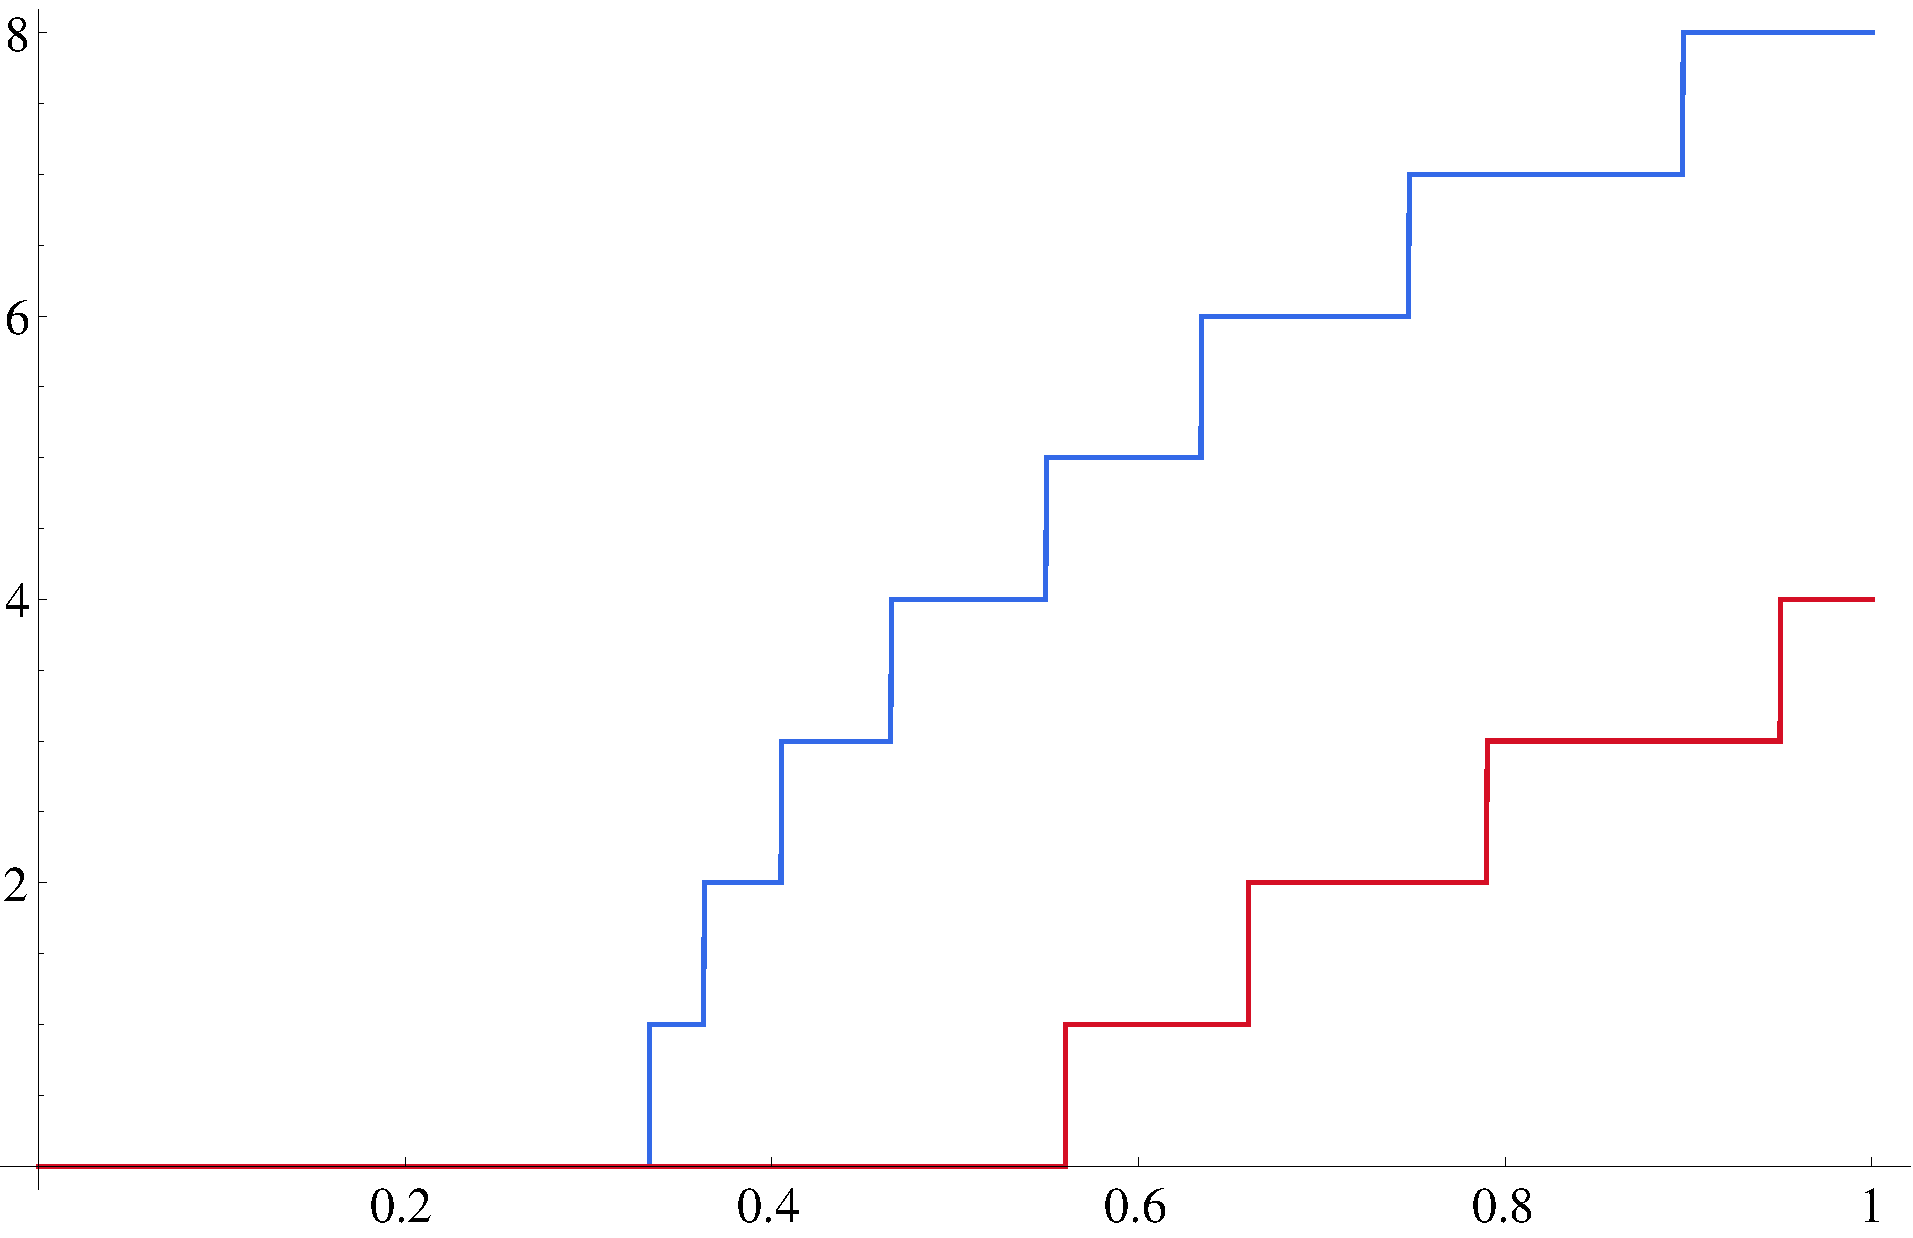
\includegraphics[width=0.8\textwidth]{./figures/plot-kL2-jL2-large.pdf}
\end{center}
\caption{Plot of the function $k_{L_{2}}(t)$ in blue and plot of the function $j_{L_{2}}(t)$ in red as functions of $t$.}
\label{fig: left-triangle-layers-estimates}
\end{figure}

% function j
In a layer with a known left boundary of a maximal cell, its right boundary is calculated either by using $f_{1,\delta}$ or by using $f_{2, \delta}$. By Proposition~\ref{prop: compare-functions-f1-f2}, there exists some $j \in \mathbb{Z}$, to which the implications
\begin{itemize}
  \item if $i \leq j$, then $\beta_{i} = f_{1,\delta}(\beta_{i-1})$;
  \item if $i > j$, then $\beta_{i} = f_{2,\delta}(\beta_{i-1})$;
\end{itemize}
apply. For some $t$, there may be a jump in the values of $j$. This only happens if:
$$
\beta_{j} = f_{1,\delta}(\beta_{j-1}) = f_{2,\delta}(\beta_{j-1}).
$$

For $m=1,2,3$ denote by $j_{L_{m}} = j_{L_{m}}(t)$ a function that counts how many times we have to use $f_{2, \delta}$ before we start using $f_{2, \delta}$ to calculate the right boundary in the layer $L_{m}$. The $j_{L_{m}}$ is also a jump-step function and we mark its discontinuity points as critical values of parameter $t$. For these values of parameter $t$, the function $k_{L_{m}}$ can have a jump, which is limited in size by 1.

For the layer $L_{2}$, the $j_{L_{2}} = j_{L_{2}}(t)$ is a jump-step function shown in Figure~\ref{fig: left-triangle-layers-estimates} in red.

In the left triangle, the number of cells in the layers increases monotonically whit $t$. Approximations for critical values of $t$ were calculated numerically using bisection. The calculation is attached in Appendix A.

For $m = 1,2,3$ in the right triangle we analogously define the layers $L_{m}'$ and functions $k_{L_{m}'}, j_{L_{m}'}$. It is easy to see that the parameters $t$ and $t' = 1 - t$ are critical or subcritical at the same time. Cumulative number of cells in layers
$$
L_{1}, L_{2}, L_{3},L_{1}', L_{2}', L_{3}',
$$
represents the estimate for the number of basis points in the left and right triangles as a function of $t$. To calculate the sum of such functions, it suffices to ensure that for a single value of $t$, at most one of the terms of the sum has a jump. If we succeed in constraining the approximately calculated critical and subcritical values of the parameters
$$
t_{1} < t_{2} < ... < t_{r}
$$
by rational numbers
$$
q_{0} < q_{1} < ... < q_{r},
$$
for which $q_{i-1} < t_{i} < q_{i}$ holds, the extreme of the sum of these step functions can be determined by calculating such a sum for all the values of $q_{i}, i = 0, ..., r$.

Figure~\ref{fig: left-and-right-layers-estimates} shows an approximate calculation of the sum $S_{k}(t)$. The function $S_{k}(t)$ reaches a maximum at
$$
q_{1} = \frac{1}{11}
$$
and the sum of the functional values $S_{k}(\frac{1}{11}) = 24$. The sum of functions is a symmetric function, therefore
$$
S_{k}(\frac{10}{11}) = 24.
$$
The estimate for the upper bound on the number of basis points in the union of the left and right triangles is consequently equal to the maximum value of the function $S_{k}$, $S_{k}(\frac{1}{11}) = 24$.

\begin{figure}
\centering
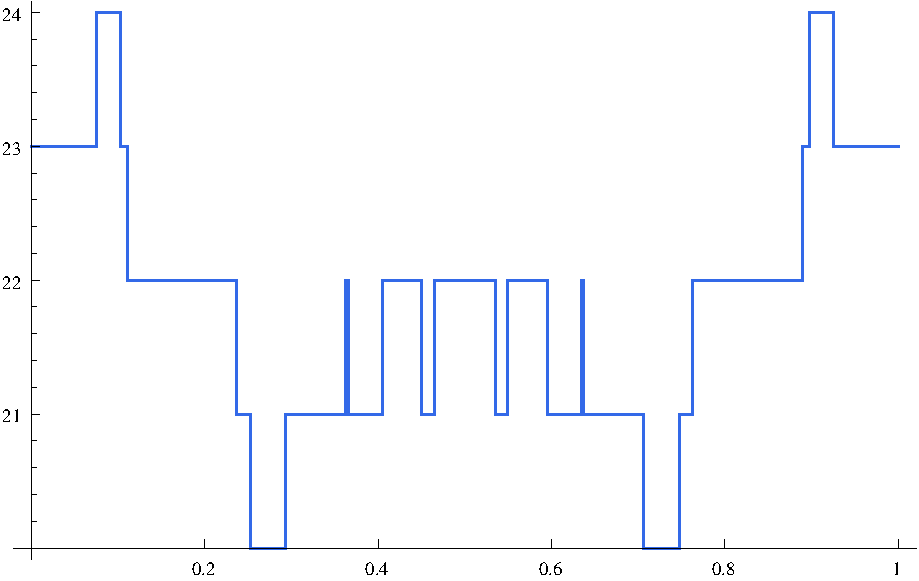
\includegraphics[width=0.8\textwidth]{./figures/left-and-right-layers-estimates-small.pdf}
\caption{Estimate for the number of basis points in the left and right triangles as a function of $t$.}
\label{fig: left-and-right-layers-estimates}
\end{figure}

The exact estimate for the whole frame $F$ will be made in the next section using the lower part $\rectansym{ab\undersym{b}\undersym{a}}$ of the frame. If both the lower and upper parts of the frame were estimated by breaking into $\trisym{abc}, \trisym{abd}$, and a pair of left and right triangles, we obtain the following suboptimal estimate. We have a maximum of 36 basis points in the central triangle. In the union of the left and right triangles, a maximum of 24 basis points. This means that the basis of the partial drawing has a maximum of
$$
2 \cdot 36 + 2 \cdot 24 + 4 = 124
$$
points. In this case, the term 4 corresponds to the contribution of the boundary points $ a, b, c, d $.


\section{Lower quadrilateral}
We choose ray coordinate system with respect to the points $a,b,c$. Lower quadrilateral $\rectansym{a\undersym{a}\undersym{b}b}$ without the shadows $S_{\overline{a}b}, S_{\overline{b}a}$ is covered with a maximum of three layers $B_{1},B_{2},B_{3}$. We define them as ray trapezoids with respect to $a, b, c$:
\begin{itemize}
\item $B_{1}$ with ray heights $1,\frac{4}{3}$;
\item $B_{2}$ with ray heights $\frac{4}{3},\frac{5}{3}$;
\item $B_{3}$ with ray heights $\frac{5}{3},2$.
\end{itemize}

In doing so, we can limit ourselves to two separate cases. If the parameter
$$
h = -\frac{d_{y}}{c_{y}} > \frac{2}{3},
$$
then all the layers $B_{m}, m = 1,2,3$ are non-empty. The upper height of layer $B_{3}$ can be set to 2, as the higher the height, the worst the upper bound. If, however
$$
h \leq \frac{2}{3},
$$
the layer $B_{3}$ is empty. The upper height of layer $B_{2}$ can be set to $\frac{5}{3}$ for the same reason.

\begin{figure}
\begin{center}
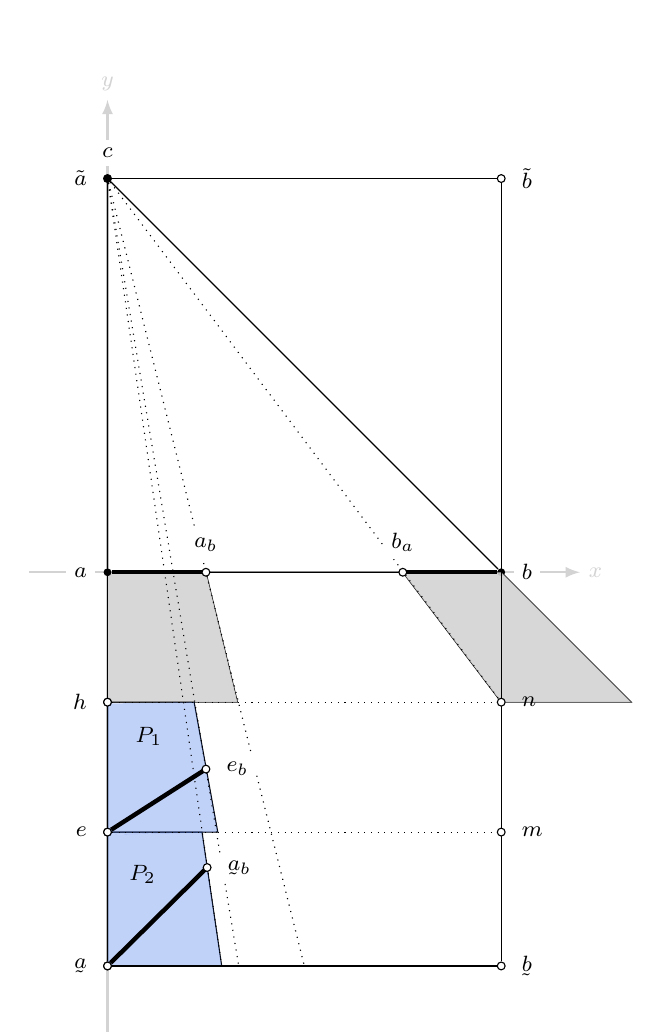
\begin{tikzpicture}[scale = 5, node distance=0.1cm,>=latex, dot/.style={circle,inner sep=1pt,fill,label={#1}, name=#1},
dot2/.style={circle,inner sep=1pt,draw,fill=white,label={#1}, name=#1}]
\begin{footnotesize}
% S_{ab}
\draw (0,0) -- (0., -0.33) -- (0.33, -0.33) -- (0.25,0) -- (0,0) -- cycle;
\fill[color-parallelogram,opacity=0.9] (0,0) -- (0., -0.33) -- (0.33, -0.33) -- (0.25,0) -- (0,0) -- cycle;

% osi
\draw[gray,thick,->] ({-.2}, 0) -- (1.2, 0) node[right] {$x$};
\draw[gray,thick,->] (0, {-1.2}) -- (0, {1.2}) node[above] {$y$};

% GeoGebra export
% since it does not change
\node[dot2=] (aabove) at (0,1) {};
\node [left = of aabove] {$\abovesym{a}$};
\node[dot2=] (abelow) at (0,-1) {};
\node [left = of abelow] {$\undersym{a}$}; %(0,-1)
\node[dot2=] (babove) at (1,1) {};
\node [right = of babove] {$\abovesym{b}$};
\node[dot2=] (bbelow) at (1,-1) {};
\node [right = of bbelow] {$\undersym{b}$};

\coordinate (ab) at (0.25,0) {};
\coordinate (ba) at (0.75,0) {};


\node[dot2=] (h) at (0,-0.33) {};
\node [left = of h] {$h$}; %(0,-\frac{1}{3})
\node[dot2=] (e) at (0,-0.66) {};
\node [left = of e] {$e$}; %(0,-\frac{2}{3})

\coordinate (ee) at (1,-0.66) {};
\coordinate (hh) at (1,-0.33) {};

\coordinate (abelowb) at ({0.25+0.003},{-0.75}) {};

\node [dot=](a) at (0,0) {};
\node [left = of a,fill=white] {$a$};
\node [dot=](b) at (1,0) {};
\node [right = of b,fill=white] {$b$};

% S_{ca}
\draw (1,0) -- (1.33, -0.33) -- (1, -0.33) -- (0.75,0) -- (1,0)  -- cycle;
\fill[color-parallelogram,opacity=0.9] (1,0) -- (1.33, -0.33) -- (1, -0.33) -- (0.75,0) -- (1,0) -- cycle;

% since it changes with t
\node [dot=](c) at (0,1) {};
\node [above = of c,fill = white] {$c$};

\coordinate (eb) at (0.25,-0.5) {};

\coordinate (g) at (0.22,-0.33) {};
\coordinate (f) at (0.28,-0.66) {};
\coordinate (fbelow) at (0.29,-1) {};
\coordinate (fcupframe) at ({0.33+0.003333},{-1}) {};
\coordinate (c14cupframe) at (0.5,-1) {};
\coordinate (c34cupframe) at (1.5,-1) {};
\coordinate (gbelow) at (0.24,-0.66) {};

% lines
%%%% color the black holes
\draw (abelow) -- (fbelow) -- (gbelow) -- (e) -- (abelow) -- cycle;
\draw (e) -- (f) -- (g) -- (h) -- (e) -- cycle;

\fill[blue,opacity=0.3] (0,-1) -- (fbelow) -- (gbelow) -- (0, {-2/3}) -- (abelow) -- cycle;
\fill[blue,opacity=0.3] (0, {-2/3}) -- (f) -- (g) -- (0,{-1/3}) -- (e) -- cycle;


% stubs
\draw[ultra thick] (a) -- (ab);
\draw[ultra thick] (b) -- (ba);
\draw[ultra thick] (abelow) -- (abelowb);
\draw[ultra thick] (e) -- (eb);

% abc and the frame
\draw [thin] (a) -- (b) -- (c) -- (a) -- cycle;
\draw [thin] (abelow) -- (bbelow) -- (babove) -- (aabove) -- (abelow) -- cycle;

% zarki iz c
\draw [dotted] (c) -- (fbelow);
\draw [dotted] (c) -- (fcupframe);
\draw [dotted] (c) -- (c14cupframe);
\draw [dotted] (c) -- (hh);

% horizontalno vzporednice ab
\draw [dotted] (h) -- (hh);
\draw [dotted] (e) -- (ee);

% end GeoGebra export

% again the dots and labels to cover the lines
\node[dot2=] (abelowb) at ({0.25+0.003},{-0.75}) {};
\node [right = of abelowb,fill=white] {$\undersym{a}_{b}$};
\node[dot2=] (eb) at (0.25,-0.5) {};
\node [right = of eb,fill = white] {$e_{b}$};
\node[dot2=] (h) at (0,-0.33) {};
\node[dot2=] (e) at (0,-0.66) {};
\node[dot2=] (abelow) at (0,-1) {};
\node[dot2=] (ab) at (0.25,0) {};
\node [above = of ab,fill=white] {$a_{b}$};
\node[dot2=] (ba) at (0.75,0) {};
\node [above = of ba,fill=white] {$b_{a}$};

\node[dot2=] (n) at (1,-0.33) {};
\node [right = of n] {$n$}; %(1,-\frac{1}{3})
\node[dot2=] (m) at (1,-0.66) {};
\node [right = of m] {$m$};%(1,-\frac{2}{3})

%%% denote P1, P2, P3
\coordinate (p1) at (0.03,{-2/3+0.25}) {};
\node [right = of p1] {$P_{1}$};

\coordinate (p2) at (0.014,{-2/3-0.1}) {};
\node [right = of p2] {$P_{2}$};


\end{footnotesize}
\end{tikzpicture}

\end{center}
\caption{Illustration at a very small value of parameter $t$.}
\label{fig: half-shadows}
\end{figure}

Let's look at the illustration for a very small value of the parameter $t$ in Figure~\ref{fig: half-shadows}. The points from the regions $P_{1}$ and $P_{2}$ have very small ray angles in RCS with respect to $a, b, c$. Therefore, to break such a layer into cells would require a large number, albeit maximal, of cells. We address the problem by dealing separately with the regions $P_ {1}$ and $P_{2}$, which will be related to the estimate for the number of points in the corner areas, which we made in Proposition~\ref{prop: corner-regions-union}.

\subsection{Half shadows}
In RCS with respect to $a,b,c$ in the lower quadrilateral $\quadsym{a\undersym{a}\undersym{b}b}$, we define four regions of special treatment called \textit{half-shadows}\footnote{A term is related to astronomy. Astronomical term is penumbra used for the shadows cast by celestial bodies.} and we denote them by
% TODO: H_1, ...
$$
P_{1},P_{2},P_{3},P_{4}.
$$

Their shape depends on the parameter $t$ (position of the point $c$). It is also possible that each of the half-shadows is empty.
Half-shadows $P_{1}, P_{3}$ lie in the layer with ray heights between $\frac{4}{3}$ and $\frac{5}{3}$, half-shadows $P_{2}, P_{4}$ in the layer with ray heights between $\frac{5}{3}$ and $2$, see Figure~\ref{fig: half-shadows-2}.

\begin{figure}
\begin{center}
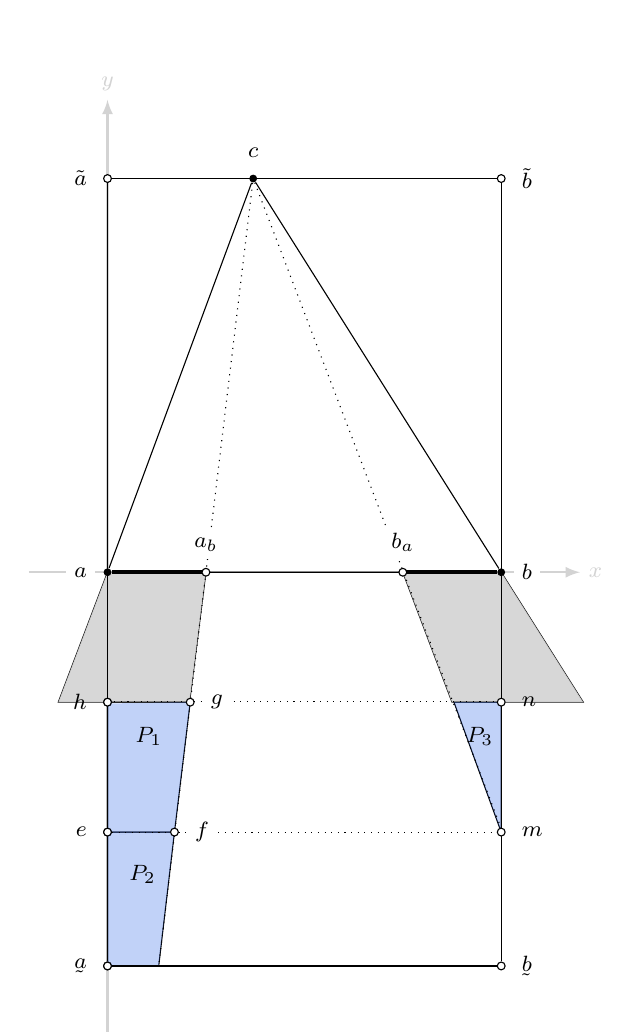
\begin{tikzpicture}[scale = 5, node distance=0.1cm,>=latex, dot/.style={circle,inner sep=1pt,fill,label={#1}, name=#1},
dot2/.style={circle,inner sep=1pt,draw,fill=white,label={#1}, name=#1}]

\begin{footnotesize}

% S_{ab}
\draw (0,0) -- (-0.125, -0.33) -- (0.208333, -0.33) -- (0.25,0) -- (0,0) -- cycle;
\fill[color-parallelogram,opacity=0.9] (0,0) -- (-0.125, -0.33) -- (0.208333, -0.33) -- (0.25,0) -- (0,0) -- cycle;

% S_{ca}
\draw (1,0) -- (1.20833, -0.33) -- (0.875, -0.33) -- (0.75,0) -- (1,0) -- cycle;
\fill[color-parallelogram,opacity=0.9] (1,0) -- (1.20833, -0.33) -- (0.875, -0.33) -- (0.75,0) -- (1,0) -- cycle;

\draw[gray,thick,->] ({-.2}, 0) -- (1.2, 0) node[right] {$x$};
\draw[gray,thick,->] (0, {-1.2}) -- (0, {1.2}) node[above] {$y$};

\node[dot2=] (aabove) at (0,1) {};
\node [left = of aabove] {$\abovesym{a}$};
\node[dot2=] (abelow) at (0,-1) {};
\node [left = of abelow] {$\undersym{a}$}; %(0,-1)
\node[dot2=] (babove) at (1,1) {};
\node [right = of babove] {$\abovesym{b}$};
\node[dot2=] (bbelow) at (1,-1) {};
\node [right = of bbelow] {$\undersym{b}$};

\coordinate (ab) at (0.25,0) {};
\coordinate (ba) at (0.75,0) {};


\node[dot2=] (h) at (0,-0.33) {};
\node [left = of h] {$h$}; %(0,-\frac{1}{3})
\node[dot2=] (e) at (0,-0.66) {};
\node [left = of e] {$e$}; %(0,-\frac{2}{3})

\coordinate (ee) at ({1},{-0.66}) {};
\coordinate (hh) at (1,-0.33) {};

\coordinate (abelowb) at ({0.25+0.003},{-0.75}) {};

\node [dot=](a) at (0,0) {};
\node [left = of a,fill=white] {$a$};
\node [dot=](b) at (1,0) {};
\node [right = of b,fill=white] {$b$};

\coordinate (c38) at (0.37,1) {};
\coordinate (g38) at (0.21,-0.33) {};
\coordinate (f38) at (0.17,-0.66) {};
\coordinate (fbelow38) at  (0.13,-1) {};
\coordinate (g38g38) at (0.88,-0.33) {};

\node [dot=](c) at (0.37,1) {};
\node [above = of c,fill = white] {$c$};

\coordinate (eb) at (0.25,-0.5) {};

\coordinate (g) at (0.21,-0.33) {};
\coordinate (f) at (0.17,-0.66) {};
\coordinate (fbelow) at (0.13,-1) {};
\coordinate (fpresekokvir) at ({0.33+0.003333},{-1}) {};
\coordinate (c14presekokvir) at (0.5,-1) {};
\coordinate (c34presekokvir) at (1.5,-1) {};
\coordinate (gbelow) at (0.24,-0.66) {};

\draw (abelow) -- (fbelow) -- (f) -- (e) -- (abelow) -- cycle;
\draw (e) -- (f) -- (g) -- (h) -- (e) -- cycle;

\fill[blue,opacity=0.3] (0,-1) -- (fbelow) -- (f) -- (0, {-2/3}) -- (abelow) -- cycle;
\fill[blue,opacity=0.3] (0, {-2/3}) -- (f) -- (g) -- (0,{-1/3}) -- (e) -- cycle;

\draw (ee) -- (hh) -- (0.88,-0.33) -- (ee) -- cycle;
\fill[blue,opacity=0.3] (ee) -- (hh) -- (0.88,-0.33) -- (ee) -- cycle;

\draw[ultra thick] (a) -- (ab);
\draw[ultra thick] (b) -- (ba);

\draw [thin] (a) -- (b) -- (c) -- (a) -- cycle;
\draw [thin] (abelow) -- (bbelow) -- (babove) -- (aabove) -- (abelow) -- cycle;

\draw [dotted] (c) -- (fbelow);
\draw [dotted] (c) -- ({1+0.001},{-0.66+0.00666});

\draw [dotted] ({0},{-1/3+0.004}) -- ({1},{-1/3+0.004});
\draw [dotted] (e) -- (ee);

\node[dot2=] (h) at (0,-0.33) {};
\node[dot2=] (e) at (0,-0.66) {};
\node[dot2=] (abelow) at (0,-1) {};
\node[dot2=] (ab) at (0.25,0) {};
\node [above = of ab,fill=white] {$a_{b}$};
\node[dot2=] (ba) at (0.75,0) {};
\node [above = of ba,fill=white] {$b_{a}$};

\node[dot2=] (n) at (1,-0.33) {};
\node [right = of n] {$n$}; %(1,-\frac{1}{3})
\node[dot2=] (m) at (1,-0.66) {};
\node [right = of m] {$m$}; %(1,-\frac{2}{3})

\coordinate (p1) at (0.03,{-2/3+0.25}) {};
\node [right = of p1] {$P_{1}$};

\coordinate (p2) at (0.014,{-2/3-0.1}) {};
\node [right = of p2] {$P_{2}$};

\coordinate (p3) at ({1-0.129},{-2/3+0.25}) {};
\node [right = of p3] {$P_{3}$};

\node[dot2=] (g) at (0.21,-0.33) {};
\node[right = of g,fill=white] {$g$};
\node[dot2=]  (f) at (0.17,-0.66) {};
\node[right = of f,fill=white] {$f$};

\end{footnotesize}
\end{tikzpicture}
\end{center}
\caption{Illustration at value $t = \frac{3}{8}$.}
\label{fig: half-shadows-2}
\end{figure}

% description of half-shadows
The half-shadow $P_{1}$ is empty for the values of the parameter $t \in (\frac{5}{8}, 1]$. For $t \in [0, \frac{5}{8}]$, the half-shadow $P_{1}$ is defined as the intersection of the frame $F$ with the ray trapezoid
$$
\tpz{\left[ 0,\varphi,\frac{4}{3},\frac{5}{3} \right]_{a,b,c} }.
$$
For $t \in [\frac{1}{4},\frac{5}{8}]$ the value of parameter $\varphi = \frac{1}{4}$. For $t \in [0, \frac{1}{4}]$ the $\varphi$ is the extreme ray angle at which for every point $p \in P_{1}$ its stub $\overline{p}b$ intersects $\varphi$-ray. It follows from Corollary~\ref{cor: consequence-of-ray-coordinates-of-umbrella-ends} that for $\varphi$ we can choose the ray angle of the ray from $c$ to the end of $e_{b}$, see Figure~\ref{fig: half-shadows}.

The half-shadow $P_{2}$ is empty for the values of parameter $t \in (\frac{3}{8}, 1]$. For $t \in [0, \frac{3}{8}]$, the half-shadow $P_{2}$ is defined as the intersection of the frame $F$ with the ray trapezoid
$$
\tpz{\left[ 0,\varphi,\frac{5}{3},2 \right]_{a,b,c} }.
$$
For $t \in [\frac{1}{4},\frac{3}{8}]$, the value of parameter is $\varphi = \frac{1}{4}$. For $t \in [0, \frac{1}{4}]$, the $\varphi$ is the extreme ray angle at which for every point $p \in P_{2}$ its stub $\overline{p}b$ intersects $\varphi$-ray. From Corollary~\ref{cor: consequence-of-ray-coordinates-of-umbrella-ends} it follows that for $\varphi$ we can choose the ray angle of the ray from $c$ to end $\undersym{a}_{b}$, see Figure~\ref{fig: half-shadows}.

The half-shadows $P_{3}, P_{4}$ are defined analogously as $P_{1}, P_{2}$ by choosing the parameter $1 - t$ and stubs towards point $a$. The treatment of half-shadows is summarized in Table~\ref{tab: half-shadows-description}.

\begin{table*}
\begin{center}
\begin{tabular}{lcc}
	\toprule[1.5pt]
    Half-shadow & $t \in $ & $\varphi$ from \\
	\midrule[1.5pt]
	$P_{1}$  & $[0,\frac{1}{4}]$ & $e_{b}$\\[0.2cm]
	$P_{1}$  & $[\frac{1}{4},\frac{5}{8}]$& $a_{b}$ \\[0.2cm]

	$P_{2}$  & $[0,\frac{1}{4}]$& $\undersym{a}_{b}$ \\[0.2cm]
	$P_{2}$ & $[\frac{1}{4},\frac{3}{8}]$ & $a_{b}$ \\[0.2cm]

	$P_{3}$ & $[\frac{3}{8},\frac{3}{4}]$ & $b_{a}$ \\[0.2cm]
	$P_{3}$ & $[\frac{3}{4},1]$ & $m_{a}$ \\[0.2cm]

	$P_{4}$ & $[\frac{5}{8},\frac{3}{4}]$ & $b_{a}$ \\[0.2cm]
	$P_{4}$ & $[\frac{3}{4},1$ & $\undersym{b}_{a}$ \\[0.2cm]
	\bottomrule[1.5pt]
\end{tabular}
\end{center}
\caption{Summary of half-shadows.}
\label{tab: half-shadows-description}
\end{table*}

% nesting and the assumption that p 'is more inward than p
Observe the half-shadow $P_{1}$ and choose any two points $p,p' \in P_{1}$. Assume that they belong to the basis $p,p' \in \Pi$. For the point $p$ its stub $\overline{p}b$ intersects the extreme ray of the region $P_{1}$ (line trough $c$ and $f$), and the stub $\overline{p}c$ intersects the line parallel to $\overline{ab}$ at ray height $\frac{5}{4}$. The same is true for $p'$. This means that the angles $\sangle{cpb}$ and $\sangle{cp'b}$ are nested and we can assume without the loss of generality that
$$
\sangle{cp'b} \subseteq \sangle{cpb}.
$$

% estimate of length quotient
Denote the vertices of half-shadow $P_{1}$ with $e,f,g,h$, see Figure~\ref{fig: half-shadows-2}. Let $r$ be the line that goes trough $p$ and $b$. We estimate the quotient of the following lengths. The length of the line segment $\overline{pb}$ and the lengths of the rectangular projection of the line segment $\overline{p'b}$ on the line $r$, denoted by $\left|\proj_{r} \left(\overline{p'b}\right) \right|$, and denote it by $q_{b}(t)$:
\begin{align*}
\frac{\left|pb\right|}{\left|\proj_{r} \left(\overline{p'b}\right)\right|} &\leq
\frac{\left|eb\right|}{\min
\left\{
\left|\proj_{\overline{fb}} \left(\overline{gb}\right)\right|,
\left|\proj_{\overline{hb}} \left(\overline{gb}\right)\right|
\right\}
} = q_{b}(t) = \\[6pt]%
&= \vertwopartdef
{ \frac{\sqrt{13}}{
3\cdot\min
\left\{ \frac{\left| 65 - 12 t \right|}{24 \sqrt{10}},
\frac{\left| 451 + 8 (1 - 2 t) t \right|}{24 \sqrt{545 + 8 t (17 + 2 t)}} \right\}
}, } {t \leq \frac{1}{4},}
{ \frac{\sqrt{13}}{
3\cdot\min
\left\{ \frac{\left| 7 + 3 t \right|}{3 \sqrt{10}},
\frac{\left| 22 + t (23 + 8 t) \right|}{3 \sqrt{113 + 16 t (7 + 4 t)}} \right\}
}, } {t \geq \frac{1}{4}.} \\[6pt]%
\end{align*}

The calculation for the expression $q_{b}$ as a function of $t$ is available in Appendix A. Let $s$ be a line passing through $p$ and $c$. Similarly, we denote by $q_{c}$ the estimate for the quotient of the length of $\overline{pc}$ and the length of the rectangular projection of the line segment $\overline{p'c}$ on $s$, denoted by $\left|\proj_{s} \left(\overline{p'c}\right) \right|$:

\begin{align*}
\frac{\left|pc\right|}{\left|\proj_{s} \left(\overline{p'c}\right)\right|} &\leq
\frac{\max\left\{ \left|ec\right|, \left|fc\right| \right\}}{\min
\left\{
\left|\proj_{\overline{gc}} \left(\overline{hc}\right)\right|,
\left|\proj_{\overline{hc}} \left(\overline{gc}\right)\right|
\right\}
} = q_{c}(t) = \\[6pt]%
&= \vertwopartdef
{
\frac{
\max
\left\{ \sqrt{\frac{25}{9} + \frac{49}{576}\left(1-4t\right)^{2}}, \sqrt{\frac{25}{9}+t^{2}} \right\}
}{
\min
\left\{ \frac{128 + 15t(4t-1)}{24 \sqrt{16+9t^{2}}},
\frac{128 + 15t(4t-1)}{3 \sqrt{1049+200t(2t-1)}} \right\}}, } {t \leq \frac{1}{4},}
{
\frac{
\max
\left\{ \frac{5}{3} \sqrt{1 + \left(t - \frac{1}{4}\right)^{2}}, \sqrt{\frac{25}{9}+t^{2}} \right\}
}{
\min
\left\{ \frac{16 + 3t(4t-1)}{3 \sqrt{16+9t^{2}}},
\frac{16 + 3t(4t-1)}{3 \sqrt{17 + 8t(2t-1)}} \right\}}, } {t \geq \frac{1}{4}.} \\[6pt]%
\end{align*}

The calculation for the expression $q_{c}$ as a function of $t$ is also available in Appendix A. With $\ell$ we denote the end of the stub $\overline{p}p'$ and define the angles:
$$
\beta' = \sangle{pbp'}, \hat{\beta} = \sangle{pbl},
$$
$$
\gamma' = \sangle{pcp'}, \hat{\gamma} = \sangle{pcl}.
$$
At least one of the inequalities holds because of nesting
$$
\beta' \geq \hat{\beta} \text{\hspace{0.8cm}   or   \hspace{0.8cm}} \gamma' \geq \hat{\gamma}.
$$

Estimate the quotient of the angles $\beta'$ and $\hat{\beta}$ assuming that $\beta' \geq \hat{\beta}$
\begin{equation}
\label{eq: half-shados-beta}
\frac{\beta'}{\hat{\beta}} \leq \frac{\tan(\beta')}{\tan(\hat{\beta})} \leq 4\cdot\frac{\left|pb\right|}{\left|\proj_{\overline{pb}} \left(\overline{p'b}\right) \right|} \leq 4 \cdot q_{b}(t).
\end{equation}

The first inequality follows due to the convexity and increasing of tangent function on $(0,\frac{\pi}{2})$. Provided that $\gamma' \geq \hat{\gamma}$, a similar relationship holds
\begin{equation}
\label{eq: half-shadows-gamma}
\frac{\gamma'}{\hat{\gamma}} \leq 4 \cdot q_{c}(t).
\end{equation}
Therefore, at least one of the estimates~\eqref{eq: half-shados-beta} or~\eqref{eq: half-shadows-gamma} holds.

Let $\left\{ p_{0},p_{1},..., p_{k} \right\}$ be the maximum family of points from the basis $\Pi$ lying in $P_{1}$. Here we can assume nesting:
$$
\sangle{cp_{k}b} \subseteq \sangle{cp_{k-1}b} \subseteq ... \subseteq \sangle{cp_{1}b} \subseteq \sangle{cp_{0}b}.
$$
For $i = 1, ..., k$ we write
$$
\beta_{i} = \sangle{p_{0}bp_{i}} \textit{  and  } \gamma_{i} = \sangle{p_{0}cp_{i}}.
$$
Similar to Preposition~\ref{prop: nesting} also for sequences $(\beta_{i})_{i}$ and $(\gamma_{i})_{i}, i = 1,...,k$ holds:
$$
\beta_{i} \geq \frac{4}{3}\beta_{i-1} \text{\hspace{0.8cm}   in   \hspace{0.8cm}} \gamma_{i} \geq \frac{4}{3} \gamma_{i-1}.
$$

The point $p_{1}$ is subject to one of the relationships:
$$
\sangle{p_{0}bp_{1}} \geq  \sangle{p_{0}b(p_{0})_{p_{k}}} \text{\hspace{0.8cm}   or   \hspace{0.8cm}} \sangle{p_{0}cp_{1}} \geq \sangle{p_{0}c(p_{0})_{p_{k}}}.
$$
In the first case, we produce an estimate
$$
\beta_{k} \leq 4 \cdot q_{b}(t) \cdot \beta_{1} \leq 4 \cdot q_{b}(t) \left(\frac{3}{4}\right)^{k-1} \cdot \beta_{k},
$$
which holds when $k \leq 7$ for $t < t_{0} \approx 0{,}4585$ and when $k \leq 6$ for $t \geq t_{0}$. For $t > \frac{5}{8}$ the half-shadow $P_{1}$ is empty. In the second case
$$
\gamma_{k} \leq 4 \cdot q_{c}(t) \cdot \gamma_{1} \leq 4 \cdot q_{c}(t) \left(\frac{3}{4}\right)^{k-1} \cdot \gamma_{k},
$$
which holds when $k \leq 6$ for each $t$ from the interval on which the half-shadow $P_{1}$ is not empty. We get a worse bound in the first of the two cases and summarize it in the next statement, taking into account the point $p_{0}$.

\begin{proposition}
In the half-shadow $P_{1}$ we have at most 8 basis points for $t < t_{0} \approx 0{,}4585$ and at most 7 for $t \geq t_{0}$. Symbolically
$$
\left|
\Pi \cap P_{1}
\right| \leq \twopartdef
{ 8, } {t < t_{0} \approx 0{,}4585,}
{ 7, } {t \geq t_{0}.}
$$
\end{proposition}

We get the critical value of $t$, which is the exact value at which the estimate drops from 8 to 7 basis points, which we limit between two rational numbers. An analogous estimate is also made for the region $P_{2}$. The half-shadows $P_{3}, P_{4}$ are derived using symmetry. The results can be summarized in a plot showing the estimate for the number of basis points in half-shadows depending on the value of parameter $t$.

\begin{figure}
\centering
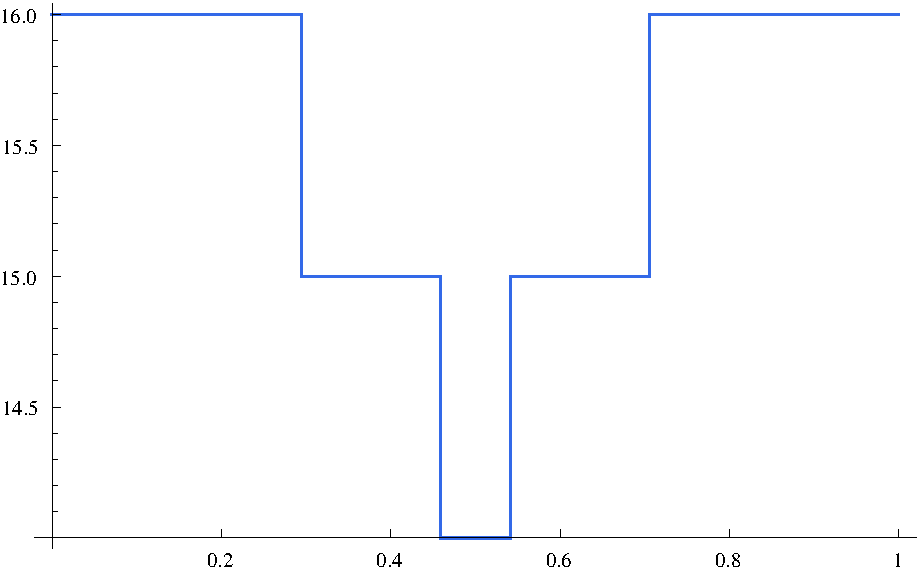
\includegraphics[width=0.8\textwidth]{./figures/estimates-in-half-shadows.pdf}
\caption{Estimate for the number of basis points in half-shadows as a function of $t$.}
\label{fig: estimates-in-half-shadows}
\end{figure}

\subsection{Lower layers}
We transform the frame again so that the central triangle $\trisym{abc}$ becomes equilateral and introduce the RCS with respect to $a,b,c$. Assume $h > \frac{2}{3}$. The lower quadrilateral $\rectansym{a\undersym{a}\undersym{b}b}$, without the shadows $S_{\overline{a}b}, S_{\overline{b}a}$ and without the half-shadows $P_{1}, P_{2}, P_{3}, P_{4}$, we cover with ray trapezoids with respect to $a,b,c$:
$$
B_{1} = \tpz{\left[ \frac{1}{4},\frac{3}{4},1,\frac{4}{3} \right]_{a,b,c} },
$$
$$
B_{2} = \tpz{\left[ \alpha_{2},\omega_{2},\frac{4}{3},\frac{5}{3} \right]_{a,c,b} },
$$
$$
B_{3} = \tpz{\left[ \alpha_{3},\omega_{3},\frac{5}{3},2 \right]_{a,c,b} }.
$$
The parameters $\alpha$ and $\omega$ in the layers $B_{2}, B_{3}$ depend on which sub-interval $t$ lies and on whether the half-shadows $P_{i}, i = 1,...,4$ are empty or non-empty.

\begin{figure}
\begin{center}
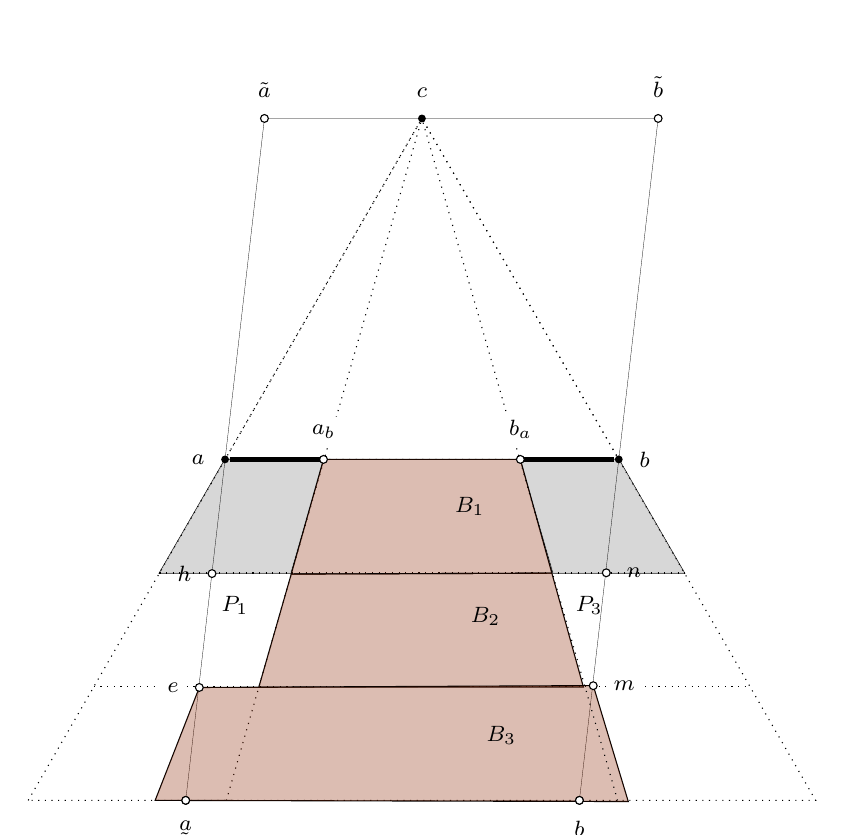
\begin{tikzpicture}[scale = 5, node distance=0.1cm,>=latex, dot/.style={circle,inner sep=1pt,fill,label={#1}, name=#1},
dot2/.style={circle,inner sep=1pt,draw,fill=white,label={#1}, name=#1}]

\begin{footnotesize}
% S_{ab}
\draw (0,0) -- (-0.166667, -0.288675) -- (0.166667, -0.288675) -- (0.25,0) -- (0,0) -- cycle;
\fill[color-parallelogram,opacity=0.9] (0,0) -- (-0.166667, -0.288675) -- (0.166667, -0.288675) -- (0.25,0) -- (0,0) -- cycle;

% S_{ba}
\draw (1,0) -- (1.16667, -0.288675) -- (0.833333, -0.288675) -- (0.75,0) -- (1,0) -- cycle;
\fill[color-parallelogram,opacity=0.9] (1,0) -- (1.16667, -0.288675) -- (0.833333, -0.288675) -- (0.75,0) -- (1,0) -- cycle;

\node [dot=](a) at (0,0) {};
\node [left = of a] {$a$};
\node [dot=](b) at (1,0) {};
\node [right = of b] {$b$};
\node [dot=](c) at ({1/2},{sqrt(3)/2}) {};
\node [above = of c] {$c$};

\coordinate (e) at (-0.06541, -0.57937) {};
\coordinate (h) at (-0.03315, -0.29366) {};
\coordinate (n) at (0.96821, -0.2816) {};
\coordinate (m) at (0.93514, -0.57456) {};
\coordinate (ab) at (0.25,0) {};
\coordinate (ba) at (0.75,0) {};

\node [dot2=](overa) at ({1/2-0.4},{sqrt(3)/2}) {};
\node [above = of overa] {$\abovesym{a}$};
\node [dot2=](overb) at ({1/2 + 0.6},{sqrt(3)/2}) {};

\node [dot2=](undera) at ({1/2-0.6},{-sqrt(3)/2}) {};
\node [below = of undera] {$\undersym{a}$};
\node [dot2=](underb) at ({1/2+0.4},{-sqrt(3)/2}) {};
\node [below = of underb] {$\undersym{b}$};

\draw[ultra thin] (undera) -- (underb) -- (overb) -- (overa) -- (undera) -- cycle;
\draw[thin,dotted] (a) -- (b) -- (c) -- (a) -- cycle;

\draw [thin,dotted] ({-1/2},{-sqrt(3)/2}) -- ({1/2},{sqrt(3)/2}) -- ({3/2},{-sqrt(3)/2}) -- cycle;

\draw [thin,dotted]({-1/3},{-sqrt(3)/3}) -- ({4/3},{-sqrt(3)/3});
\draw [thin,dotted]({-1/6},{-sqrt(3)/6}) -- ({7/6},{-sqrt(3)/6});

\draw [thin,dotted] (c) -- (0.00332, -0.86603);

\draw[ultra thick] (a) -- ({0.25},0);
\draw[ultra thick] ({0.75}, 0) -- (b);


\coordinate (e) at (-0.06541, -0.57937) {};
\coordinate (h) at (-0.03315, -0.29366) {};
\coordinate (n) at (0.96821, -0.2816) {};
\coordinate (m) at (0.93514, -0.57456) {};

\coordinate (f) at (0.16815, -0.29124) {};
\coordinate (g) at (0.08573, -0.57864) {};
\coordinate (ff) at (0.83, -0.289) {};
\coordinate (gg) at (0.91, -0.578) {};
\coordinate (uu) at (0.997, -0.86603) {};

% B1
\draw[] (ab) -- (ba) -- (ff) -- (f) -- (ab)-- cycle;
\fill[red,opacity=0.3] (ab) -- (ba) -- (ff) -- (f) -- (ab)-- cycle;

% B2
\draw[] (ff) -- (f) -- (g)-- (gg) -- (ff)-- cycle;
\fill[red,opacity=0.3] (ff) -- (f) -- (g)-- (gg) -- (ff)-- cycle;

% B3
\draw[] (1.02407, -0.869) -- (m)-- (e) --(-0.17754, -0.86603) --(1.02407, -0.869) -- cycle;
\fill[red,opacity=0.3] (1.02407, -0.869) -- (m)-- (e) -- (-0.17754, -0.86603) --(1.02407, -0.869) -- cycle;

\draw[thin,dotted] (c) -- (uu);

\node [dot2=](e) at (-0.06541, -0.5793) {};
\node [left = of e,fill=white] {$e$};
\node [dot2=](h) at (-0.03315, -0.29) {};
\node [left = of h] {$h$};
\node [dot2=](n) at (0.96821, -0.288) {};
\node [right = of n] {$n$};
\node [dot2=](m) at (0.93514, -0.5748) {};
\node [right = of m,fill=white] {$m$};
\node[dot2=] (ab) at (0.25,0) {};
\node [above = of ab,fill=white] {$a_{b}$};
\node[dot2=] (ba) at (0.75,0) {};
\node [above = of ba,fill=white] {$b_{a}$};
\node [above = of overb,fill=white] {$\abovesym{b}$};

%%% P1,P2,P3
\coordinate (p1) at (0.1,{-0.33-0.04}) {};
\node [left = of p1] {$P_{1}$};

\coordinate (p2) at (0.85,{-0.33-0.04}) {};
\node [right = of p2] {$P_{3}$};
% Bi
\coordinate (b1) at (0.7,{-0.12}) {};
\node [left = of b1] {$B_{1}$};
\coordinate (b2) at (0.74,{-0.33-0.07}) {};
\node [left = of b2] {$B_{2}$};
\coordinate (b3) at (0.78,{-0.66-0.04}) {};
\node [left = of b3] {$B_{3}$};

\node [dot2=](undera) at ({1/2-0.6},{-sqrt(3)/2}) {};
\node [dot2=](underb) at ({1/2+0.4},{-sqrt(3)/2}) {};

\end{footnotesize}
\end{tikzpicture}
\end{center}
\caption{Lower layers at $t = 0.4$}
\label{fig: lower-layers}
\end{figure}

\begin{table*}
\begin{center}
\begin{tabular}{lccccc}
	\toprule[1.5pt]
    Layer & $t \in $ & $\alpha$ from & $\omega$ from & $\alpha$ & $\omega$ \\
	\midrule[1.5pt]
	$B_{2}$ & $(0, \frac{1}{4}]$           & $e_{b}$ & $\overline{\undersym{b}b}$ & $\frac{1+3t}{7}$ & $\frac{3+2t}{5}$ \\[0.2cm]
	$B_{2}$ & $(\frac{1}{4}, \frac{3}{8}]$ & $a_{b}$ & $\overline{\undersym{b}b}$ & $\frac{1}{4}$ & $\frac{3+2t}{5}$ \\[0.2cm]
	$B_{2}$ & $(\frac{3}{8}, \frac{1}{2}]$ & $a_{b}$ & $b_{a}$ 				     & $\frac{1}{4}$ & $\frac{3}{4}$ \\[0.2cm]

	$B_{3}$ & $(0, \frac{1}{4}]$           & $\undersym{a}_{b}$         & $\overline{\undersym{b}b}$ & $\frac{1+4t}{8}$ & $\frac{1+t}{2}$ \\[0.2cm]
	$B_{3}$ & $(\frac{1}{4}, \frac{3}{8}]$ & $a_{b}$                    & $\overline{\undersym{b}b}$ & $\frac{1}{4}$ & $\frac{1+t}{2}$ \\[0.2cm]
	$B_{3}$ & $(\frac{3}{8}, \frac{1}{2}]$ & $\overline{\undersym{a}a}$ & $\overline{\undersym{b}b}$ & $\frac{t}{2}$ & $\frac{1+t}{2}$ \\[0.2cm]
	\bottomrule[1.5pt]
\end{tabular}
\end{center}
\caption{Left and right boundaries of lower layers $B_{2}, B_{3}$.}
\label{tab: left-and-right-borders-of-lower-layers}
\end{table*}

The first lower layer $B_{1}$ lies between the shadows $S_{\overline{a}b}, S_{\overline{b}a}$. After the transformation that achieves the equilaterality of the triangle $\trisym{abc}$, the shape and size of layer $B_{1}$ are independent of $t$. Therefore, using Proposition~\ref{prop: inner-layer}, we can derive an estimate
$$
\left|
B_{1} \cap \Pi
\right| \leq 7.
$$

For the remaining two layers, however, the left and right boundaries depend on $t$. By symmetry, the lower layers can be considered only for $t \in [0,\frac{1}{2}]$. For $t$, where half-shadow $P_{1}$ is nonempty, the left boundary of the layer $B_{2}$ will be the right leg of half-shadow $P_{1}$, determined by the end of stub $e_{b}$ or by end of stub $a_{b}$. For other values of $t$, the boundaries will be defined by the sides $\overline{\undersym{a}a}, \overline{\undersym{b}b}$ of the frame $F$. The same is true for the lower layer $B_{3}$. The left and right boundaries of the layers $B_{2}, B_{3}$ are summarized in Table~\ref{tab: left-and-right-borders-of-lower-layers}. In Table we have listed where from where we get $\alpha$ and $\omega$ and how they depend on the parameter $t = c_{y}$.

Let $k_{2}$ and $k_{3}$ be estimates for the upper bound on the number of basis points located in lower layers $B_{2}$ and $B_{3}$ respectively. For a fixed $t$ we can calculate
$$
k_{B_{2}}(t),j_{B_{2}}(t),k_{B_{3}}(t),j_{B_{3}}(t),
$$
which, however, are generally no longer monotonous functions. Therefore, we need to find the critical values of the parameter $t$ analytically. In Figure~\ref{fig: lower-layer-kj} we have drawn the approximate behavior of the function $k_{B_{3}}(t)$ in blue and $j_{B_{3}}(t)$ in red for the layer $B_{3}$. The larger jump of 4 occurs due to a different definition of half-shadows when passing over $t = \frac{3}{8}$.

\begin{figure}
\centering
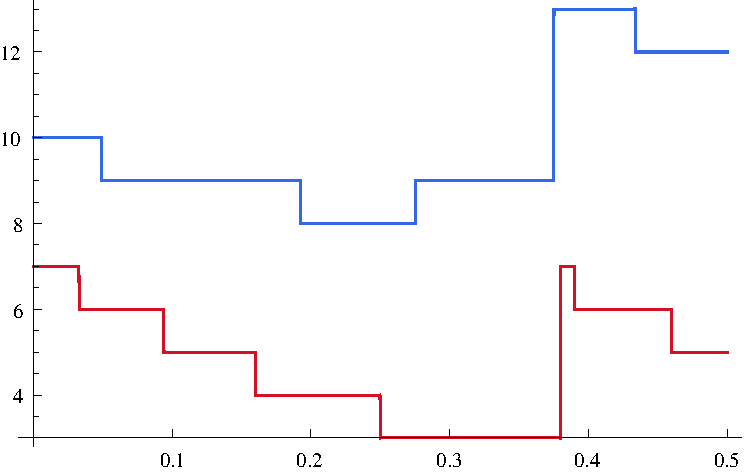
\includegraphics[width=0.8\textwidth]{./figures/lower-layer-kj.pdf}
\caption{Plot of the function $k_{B_{3}}(t)$ in blue and the function $j_{B_{3}}(t)$ in red as functions of $t$.}
\label{fig: lower-layer-kj}
\end{figure}

For an individual layer $B_{m}$, for $m = 2,3$, we first find the critical values of $t$, for which there are jumps in the value of $j_{B_{m}}(t)$. By Proposition~\ref{prop: compare-functions-f1-f2} we have
\begin{align*}
\beta_{i} &= \frac{3\delta}{1+6\delta}, \\[6pt]%
\left(\frac{1+3\delta}{3\delta}\right)^{i}\beta_{0} &= \frac{3\delta}{1+6\delta}, \\[6pt]%
\alpha(t) &= \frac{3\delta}{1+6\delta}\left(\frac{3\delta}{1+3\delta}\right)^{i}
\end{align*}
and the value of the parameter $t$ can be calculated as the inverse value of the linear function of the left boundary.
\begin{equation}
\label{eq: inverse}
t = \overset{-1}{\alpha}\left( \frac{\left(3\delta\right)^{i+1}}{(1+6\delta)\left(1+3\delta\right)^{i}} \right).
\end{equation}

For an individual layer $B_{m}, m = 2,3$, the adjacent critical values of parameter $t$, which are calculated using~\ref{eq: inverse}, are denoted by $t_{0}$ and $t_{1}$. Function $j_{B_{m}}$ is constant on the sub-interval
$$
t \in (t_{0}, t_{1}).
$$

The height $\delta$ of each individual layer is constant. Therefore, we can calculate all critical values of $t$, where the value of $k_{B_{m}}(t)$ changes. On each sub-interval between adjacent evaluations of $t$ we check whether there is a change in the number of cells $k = k_{B_{m}}(t)$. As in the proof of Proposition~\ref{prop: inner-layer}, for some fixed $t \in (t_{0}, t_{1})$, we can calculate the cell boundaries $\beta_{i}, i = 1,...,k$ and determine the value of $k_{B_{m}}(t)$. On the sub-interval $(t_{0}, t_{1})$ the critical value of $t$ occurs in two cases. In the first case, when the number of cells in the layer is reduced and $\beta_{k-1}(t)$ reaches $\omega(t)$ and the value of $k_{B_{m}}(t)$ decreases by 1. To find the critical value of $t$, we need to solve the equation
$$
\beta_{k-1}(t) = \omega(t).
$$

In the second case, however, the number of cells in the layer increases and $\omega(t)$ exceeds $\beta_{k}(t)$ and the value of $k_{B_{m}}(t)$ increases by 1. To find the critical $t$, we need to solve the equation
$$
\omega(t) = \beta_{k}(t).
$$

Specifically, there are two sub-cases in the second case. If
$$
k-1 > j_{B_{m}}(t) \text{\hspace{0.8cm}   for   \hspace{0.8cm}} t \in (t_{0}, t_{1}),
$$
then $\beta_{k}(t)$ is calculated using $f_{1,\delta}$, otherwise using $f_{2, \delta}$. The functions of left and right boundary are linear. The functions $f_{1,\delta}, f_{2,\delta}$ from the expression for $\beta_{i}$ are also linear. Therefore, $\beta_{i}$ is linear because it is a composite of $i$ linear functions. We find the critical value of $t$ by finding the intersection of two linear functions on the observed sub-interval. If there is no intersection on the sub-interval, then there is no critical value of $t$.

\chapter{Conclusion}
Appendix A provides a calculation to arrive at all critical values of the parameter $t$. These are the values of $t$ where one of the step function that estimates the number of cells in the layers or the number of basis points in the half-shadows has a jump. The approximations of the critical values $t_{r}, r = 1, ..., 43$ of parameter $t$ are:

\begin{align*}
&0.049, \text{\hspace{0.2cm}} 0.075, \text{\hspace{0.2cm}}
0.1, \text{\hspace{0.2cm}} 0.11, \text{\hspace{0.2cm}} 0.19, \text{\hspace{0.2cm}} 0.24, \text{\hspace{0.2cm}} 0.25, \text{\hspace{0.2cm}} 0.25, \text{\hspace{0.2cm}} 0.28, \text{\hspace{0.2cm}} 0.29, \text{\hspace{0.2cm}} 0.29,  \\[6pt]%
&0.33, \text{\hspace{0.2cm}} 0.35, \text{\hspace{0.2cm}} 0.36, \text{\hspace{0.2cm}} 0.37, \text{\hspace{0.2cm}} 0.38, \text{\hspace{0.2cm}} 0.40, \text{\hspace{0.2cm}} 0.43, \text{\hspace{0.2cm}} 0.45, \text{\hspace{0.2cm}} 0.46, \text{\hspace{0.2cm}} 0.47, \text{\hspace{0.2cm}} 0.50.  \\[6pt]
&0.53, \text{\hspace{0.2cm}} 0.54, \text{\hspace{0.2cm}} 0.55, \text{\hspace{0.2cm}} 0.57, \text{\hspace{0.2cm}} 0.60, \text{\hspace{0.2cm}} 0.63, \text{\hspace{0.2cm}} 0.63, \text{\hspace{0.2cm}} 0.64, \text{\hspace{0.2cm}} 0.65, \text{\hspace{0.2cm}} 0.67, \text{\hspace{0.2cm}} 0.71,  \\[6pt]%
&0.71, \text{\hspace{0.2cm}} 0.72, \text{\hspace{0.2cm}} 0.75, \text{\hspace{0.2cm}} 0.75, \text{\hspace{0.2cm}} 0.76, \text{\hspace{0.2cm}} 0.81, \text{\hspace{0.2cm}} 0.89, \text{\hspace{0.2cm}} 0.90, \text{\hspace{0.2cm}} 0.93, \text{\hspace{0.2cm}} 0.95.
\end{align*}

To calculate the sum of all such functions, it suffices to ensure that for an individual value of $t$, at most one of the terms of the sum has a jump. The approximately calculated critical values of the parameter $t$ are limited by the rational numbers $q_{r}, r = 0, ..., 43$:

\begin{align*}
&\frac{1}{40}, \text{\hspace{0.2cm}} \frac{ 1}{16}, \text{\hspace{0.2cm}} \frac{ 1}{11}, \text{\hspace{0.2cm}} \frac{ 2}{19}, \text{\hspace{0.2cm}} \frac{ 1}{6}, \text{\hspace{0.2cm}} \frac{ 1}{5}, \text{\hspace{0.2cm}} \frac{ 5}{21}, \text{\hspace{0.2cm}} \frac{ 26}{103}, \text{\hspace{0.2cm}} \frac{ 3}{11}, \text{\hspace{0.2cm}} \frac{ 2}{7}, \text{\hspace{0.2cm}} \frac{ 5}{17}, \text{\hspace{0.2cm}}\\[6pt]%
&\frac{3}{10}, \text{\hspace{0.2cm}} \frac{ 6}{17}, \text{\hspace{0.2cm}} \frac{ 5}{14}, \text{\hspace{0.2cm}} \frac{ 4}{11}, \text{\hspace{0.2cm}} \frac{ 7}{19}, \text{\hspace{0.2cm}} \frac{ 2}{5}, \text{\hspace{0.2cm}} \frac{ 3}{7}, \text{\hspace{0.2cm}} \frac{ 4}{9}, \text{\hspace{0.2cm}} \frac{ 5}{11}, \text{\hspace{0.2cm}} \frac{ 6}{13}, \text{\hspace{0.2cm}} \frac{ 7}{15}, \text{\hspace{0.2cm}}\\[6pt]%
&\frac{ 8}{15}, \text{\hspace{0.2cm}} \frac{7}{13}, \text{\hspace{0.2cm}} \frac{ 6}{11}, \text{\hspace{0.2cm}} \frac{ 5}{9}, \text{\hspace{0.2cm}} \frac{ 4}{7}, \text{\hspace{0.2cm}} \frac{ 3}{5}, \text{\hspace{0.2cm}} \frac{ 12}{19}, \text{\hspace{0.2cm}} \frac{ 7}{11}, \text{\hspace{0.2cm}} \frac{ 9}{14}, \text{\hspace{0.2cm}} \frac{ 11}{17}, \text{\hspace{0.2cm}} \frac{ 7}{10}, \text{\hspace{0.2cm}} \\[6pt]%
&\frac{ 12}{17}, \text{\hspace{0.2cm}} \frac{5}{7}, \text{\hspace{0.2cm}} \frac{ 8}{11}, \text{\hspace{0.2cm}} \frac{ 77}{103}, \text{\hspace{0.2cm}} \frac{ 16}{21}, \text{\hspace{0.2cm}} \frac{ 4}{5}, \text{\hspace{0.2cm}} \frac{ 5}{6}, \text{\hspace{0.2cm}} \frac{ 17}{19}, \text{\hspace{0.2cm}} \frac{ 9}{10}, \text{\hspace{0.2cm}} \frac{ 13}{14}, \text{\hspace{0.2cm}} \frac{ 20}{21}, \text{\hspace{0.2cm}}
\end{align*}

where each approximation of the critical value $t_{i}$
$$
q_{i-1} < t_{i} < q_{i}
$$
holds. To the sum of step functions that estimate the number of cells in the layers or the number of basis points in the half-shadows, we have added the estimate for the number of points in the central triangle when $h \geq \frac{2}{3}$, see Figure~\ref{fig: all-together-more-than-two-thirds}. The extremum of this function is determined by calculating such a sum for all values of $q_{r}, r = 1,..., 44$. We get the value 101 and our main result, which is summarized by the Theorem~\ref{thm: main}. However, if $h \leq \frac{2}{3}$, we get an estimate of 91. The function obtained in this case is in Figure~\ref{fig: all-together-less-than-two-thirds}.

In Figure~\ref{fig: coverage-mapped} is the division of the frame at one of the critical values $t = \frac{1}{11}$ and $h \geq \frac{2}{3}$, where we get the estimate 101. In Figure~\ref{fig: coverage-final-cells} is the same frame division without using the transformation at the same value of $t$. In Figure~\ref{fig: coverage-final-numbers}, we have marked each region with the maximum number of points it can contain.

\begin{figure}
\centering
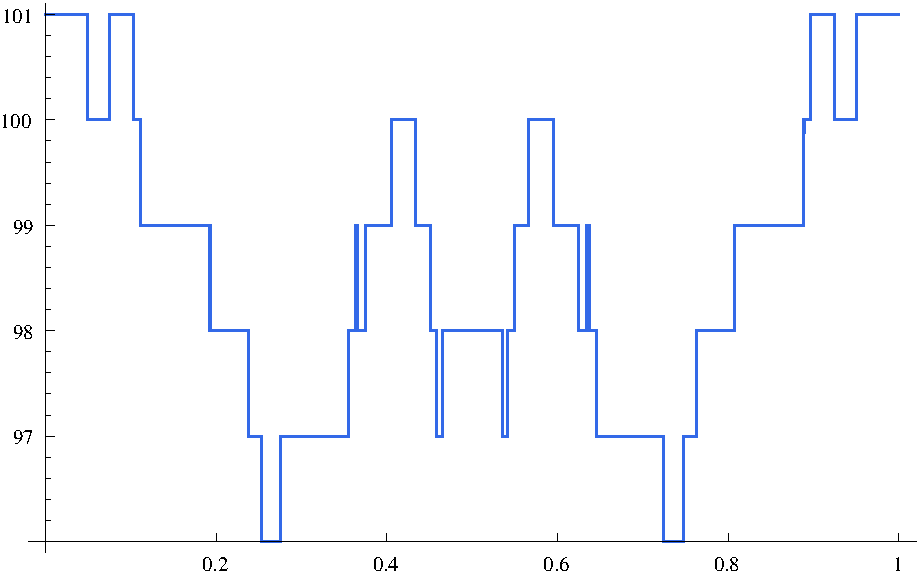
\includegraphics[width=0.8\textwidth]{./figures/all-together-more-than-two-thirds.pdf}
\caption{Plot of the estimate of the number of basis points for $h \geq \frac{2}{3}$.}
\label{fig: all-together-more-than-two-thirds}
\end{figure}

\begin{figure}
\centering
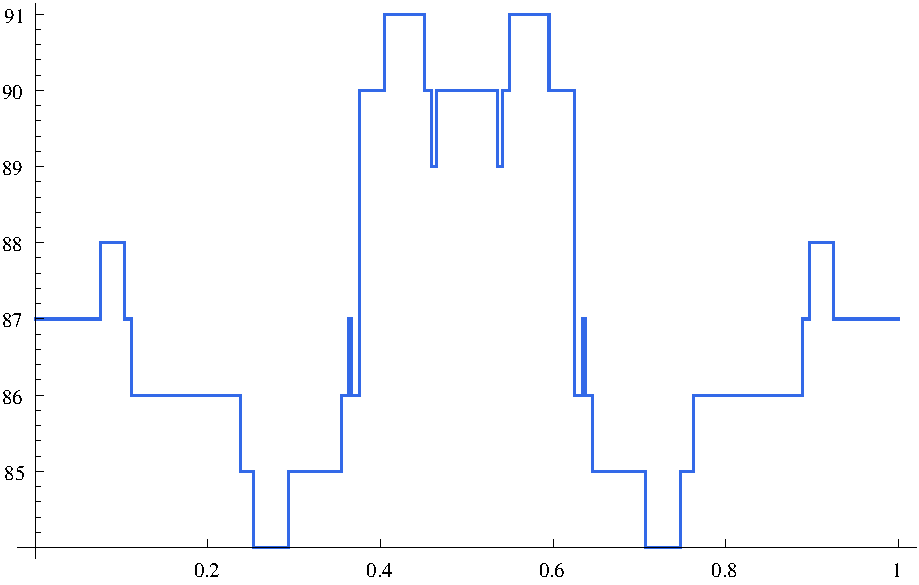
\includegraphics[width=0.8\textwidth]{./figures/all-together-less-than-two-thirds.pdf}
\caption{Plot of the estimate of the number of basis points for $h < \frac{2}{3}$.}
\label{fig: all-together-less-than-two-thirds}
\end{figure}

\begin{figure}
\centering
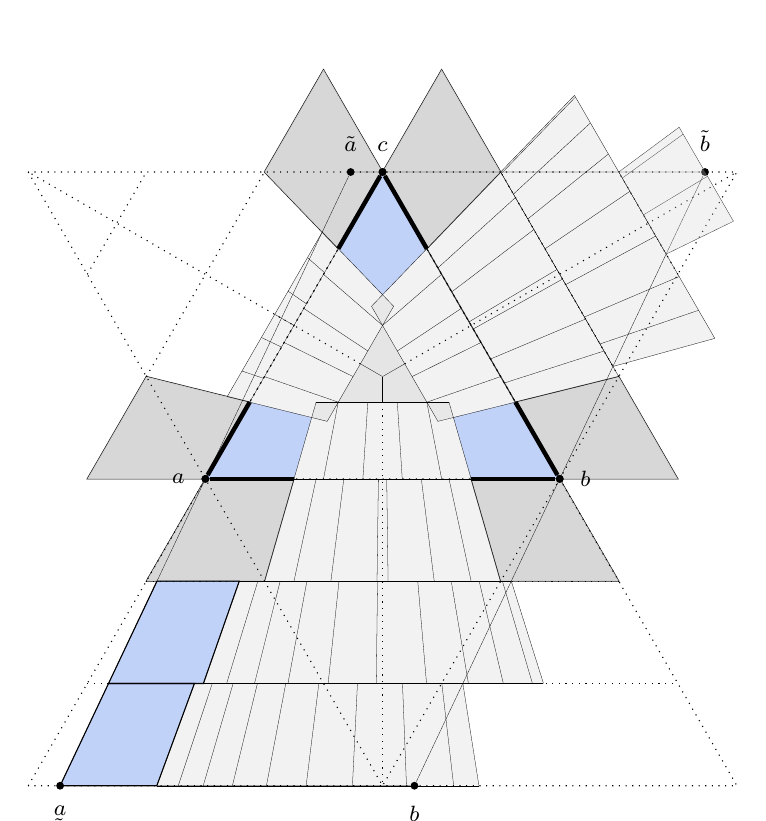
\begin{tikzpicture}[scale = 4.5, node distance=0.1cm,>=latex, dot/.style={circle,inner sep=1pt,fill,label={#1}, name=#1},
  extended line/.style={shorten >=-#1,shorten <=-#1},
 extended line/.default=1cm]
% S_{ab}
\draw (0,0) -- (-0.166667, -0.288675) -- (0.166667, -0.288675) -- (0.25,0) -- (0,0) -- cycle;
\fill[color-parallelogram,opacity=0.9] (0,0) -- (-0.166667, -0.288675) -- (0.166667, -0.288675) -- (0.25,0) -- (0,0) -- cycle;
% S_{ba}
\draw (1,0) -- (1.16667, -0.288675) -- (0.833333, -0.288675) -- (0.75,0) -- (1,0) -- cycle;
\fill[color-parallelogram,opacity=0.9] (1,0) -- (1.16667, -0.288675) -- (0.833333, -0.288675) -- (0.75,0) -- (1,0) -- cycle;

% S_{bc}
\draw (1,0) -- (1.33333, 0.) -- (1.16667, 0.288675) -- (0.875, 0.216506) -- (1,0) -- cycle;
\fill[color-parallelogram,opacity=0.9] (1,0) -- (1.33333, 0.) -- (1.16667, 0.288675) -- (0.875, 0.216506) -- (1,0) -- cycle;
% S_{cb}
\draw (0.5, 0.866025) -- (0.666667, 1.1547) -- (0.833333, 0.866025) -- (0.625, 0.649519) -- (1,0) -- cycle;
\fill[color-parallelogram,opacity=0.9] (0.5, 0.866025) -- (0.666667, 1.1547) -- (0.833333, 0.866025) -- (0.625, 0.649519) -- (1,0) -- cycle;

% S_{ac}
\draw (0,0) -- (-0.333333, 0.) -- (-0.166667, 0.288675) -- (0.125, 0.216506) -- (0,0) -- cycle;
\fill[color-parallelogram,opacity=0.9] (0,0) -- (-0.333333, 0.) -- (-0.166667, 0.288675) -- (0.125, 0.216506) -- (0,0) -- cycle;
% S_{ca}
\draw (0.5, 0.866025) -- (0.333333, 1.1547) -- (0.166667, 0.866025) -- (0.375, 0.649519) -- (0.5, 0.866025) -- cycle;
\fill[color-parallelogram,opacity=0.9] (0.5, 0.866025) -- (0.333333, 1.1547) -- (0.166667, 0.866025) -- (0.375, 0.649519) -- (0.5, 0.866025) -- cycle;

% color CL
\fill[blue, opacity=0.3] ({-0.2733333333333333}, {-0.5773502691896257}) -- ({-0.00555556},{-0.5773502691896257}) -- ({0.0955556},{-0.28867513459481287})  -- ({-0.13666666666666666},{-0.28867513459481287}) --  ({-0.2733333333333333}, {-0.5773502691896257}) -- cycle;
\fill[blue, opacity=0.3] ({-0.41000000000000003},{-0.8660254037844386})  -- ({-0.137143},{-0.866025}) -- ({-0.0309524},{-0.57735}) -- ({-0.2733333333333333}, {-0.5773502691896257}) -- ({-0.41000000000000003},{-0.8660254037844386}) -- cycle;

% color trapezoids
\fill[grey, opacity=0.3] ({0.3125},{0.2165063509}) -- ({0.2500000000},{0}) -- ({0.7500000000},{0}) -- ({0.6875},{0.2165063509}) -- cycle;
\fill[grey, opacity=0.3] ({0.46875},{0.4871392896}) -- ({0.625},{0.6495190528}) -- ({0.875},{0.2165063509})-- ({0.65625},{0.1623797632}) -- cycle;
\fill[grey, opacity=0.3] ({0.53125},{0.4871392896}) -- ({0.375},{0.6495190528}) -- ({0.125},{0.2165063509}) -- ({0.34375},{0.1623797632}) -- cycle;

\fill[grey, opacity=0.3] ({0.2500000000},{0}) -- ({0.166667},{-0.2886751346}) -- ({0.833333},{-0.2886751346})--({0.7500000000},{0}) -- cycle;

\fill[grey, opacity=0.3] ({0.0955556},{-0.288675}) -- ({-0.00555556},{-0.57735}) -- ({0.954167},{-0.57735})--({0.863333},{-0.288675})-- cycle;
\fill[grey, opacity=0.3] ({-0.0309524},{-0.57735}) -- ({-0.137143},{-0.866025})-- ({0.772},{-0.866025})--({0.726667},{-0.57735}) -- cycle;
\fill[grey, opacity=0.3] ({0.375},{0.6495190528}) -- ({0.329759},{0.696535})-- ({0.0616622},{0.232178})--({0.125},{0.2165063509}) -- cycle;
\fill[grey, opacity=0.3] ({0.875},{0.2165063509}) -- ({1.16667},{0.2886751346}) -- ({0.833333},{0.8660254038})--({0.625},{0.6495190528})-- cycle;
\fill[grey, opacity=0.3] ({1.15018},{0.317225}) -- ({1.43773},{0.396532}) -- ({1.04167},{1.082531755})--({0.833333},{0.8660254038})-- cycle;

% color parallelograms
\node [dot=](a) at (0,0) {};
\node [dot=](b) at (1,0) {};
\node [dot=](c) at ({1/2},{sqrt(3)/2}) {};

%% color deltoids
% deltoid_a
\fill[blue, opacity=0.3] (0,0) -- (0.25,0) -- (0.3, 0.173205) -- (0.125, 0.216506) -- (0,0) -- cycle;
% deltoid_b
\fill[blue, opacity=0.3] (0.75,0) -- (1,0) -- (0.875, 0.216506) -- (0.7, 0.173205) -- (0.75,0) -- cycle;
% deltoid_c
\fill[blue, opacity=0.3] (0.5, 0.866025) -- (0.625, 0.649519) -- (0.5, 0.519615) -- (0.375, 0.649519) -- (0.5, 0.866025) -- cycle;

% color inside
\fill[grey, opacity=0.6] ({0.375}, {sqrt(3)/8}) -- ({0.625}, {sqrt(3)/8}) -- ({0.5}, {sqrt(3)/4}) -- cycle;
\begin{footnotesize}
\node [dot=](a) at (0,0) {};
\node [left = of a] {$a$};
\node [dot=](b) at (1,0) {};
\node [right = of b] {$b$};
\node [dot=](c) at ({1/2},{sqrt(3)/2}) {};
\node [above = of c] {$c$};

\node [dot=](overa) at ({1/2-0.09},{sqrt(3)/2}) {};
\node [above = of overa] {$\abovesym{a}$};
\node [dot=](overb) at ({1/2 + 0.91},{sqrt(3)/2}) {};

\node [dot=](undera) at ({1/2-0.91},{-sqrt(3)/2}) {};
\node [below = of undera] {$\undersym{a}$};
\node [dot=](underb) at ({1/2+0.09},{-sqrt(3)/2}) {};
\node [below = of underb] {$\undersym{b}$};

%[semithick,black]
\draw[ultra thin] (undera) -- (underb) -- (overb) -- (overa) -- (undera) -- cycle;
\draw[thin,dotted] (a) -- (b) -- (c) -- (a) -- cycle;

% big triangle
\draw [thin,dotted] ({-1/2},{-sqrt(3)/2}) -- ({1/2},{sqrt(3)/2}) -- ({3/2},{-sqrt(3)/2}) -- cycle;
% flipud
\draw [thin,dotted] ({-1/2},{sqrt(3)/2}) -- ({1/2},{-sqrt(3)/2}) -- ({3/2},{sqrt(3)/2}) -- cycle;
% draw lower two lines and upper four tilted lines
\draw [thin,dotted]({-1/3},{-sqrt(3)/3}) -- ({4/3},{-sqrt(3)/3});
\draw [thin,dotted]({-1/6},{-sqrt(3)/6}) -- ({7/6},{-sqrt(3)/6});
\draw [thin,dotted]({-1/3},{sqrt(3)/3}) -- ({-1/6},{sqrt(3)/2});
\draw [thin,dotted]({-1/6},{sqrt(3)/6}) -- ({1/6},{sqrt(3)/2});
\draw [thin,dotted]({7/6},{sqrt(3)/6}) -- ({5/6},{sqrt(3)/2});
\draw [thin,dotted]({4/3},{sqrt(3)/3}) -- ({7/6},{sqrt(3)/2});
% halfs frmo 3/4 outwards
\draw [thin,dotted] ({0.5}, {0.2165063509461096}) -- ({1/2},{-sqrt(3)/2});
\draw [ thin,dotted] ({0.5625}, {0.3247595264191645}) -- ({3/2},{sqrt(3)/2});
\draw [ thin,dotted] ({0.4375}, {0.3247595264191645}) -- ({-1/2},{sqrt(3)/2});
% inside deltoids
\draw [ultra thin] ({0.5}, {0.2165063509461096}) -- ({0.5}, {0.28867513459481287});
\draw [ultra thin] ({0.5625}, {0.3247595264191645}) -- ({0.5}, {0.28867513459481287});
\draw [ultra thin] ({0.4375}, {0.3247595264191645}) -- ({0.5}, {0.28867513459481287});

% stubs
\draw[ultra thick] (b) -- ({1 - 0.25*(0.5)}, {0.25*sqrt(3)/2});
\draw[ultra thick] ({1 - 0.75*(0.5)}, {0.75*sqrt(3)/2}) -- (c);
\draw[ultra thick] (a) -- ({0.25*(0.5)}, {0.25*sqrt(3)/2});
\draw[ultra thick] ({0.75*(0.5)}, {0.75*sqrt(3)/2}) -- (c);
\draw[ultra thick] (a) -- ({0.25},0);
\draw[ultra thick] ({0.75}, 0) -- (b);

% symmetrically inside
\draw [ultra thin] ({0.3125},{0.2165063509}) -- ({0.2500000000},{0});
\draw [ultra thin] ({0.375},{0.2165063509}) -- ({0.3333333333},{0});
\draw [ultra thin] ({0.458333},{0.2165063509}) -- ({0.4444444444},{0});
\draw [ultra thin] ({0.541667},{0.2165063509}) -- ({0.5555555556},{0});
\draw [ultra thin] ({0.625},{0.2165063509}) -- ({0.6666666667},{0});
\draw [ultra thin] ({0.6875},{0.2165063509}) -- ({0.7500000000},{0});
\draw [ultra thin] ({0.3125},{0.2165063509}) -- ({0.6875},{0.2165063509});

\draw [ultra thin] ({0.46875},{0.4871392896}) -- ({0.625},{0.6495190528});
\draw [ultra thin] ({0.5},{0.4330127019}) -- ({0.666667},{0.5773502692});
\draw [ultra thin] ({0.541667},{0.3608439182}) -- ({0.722222},{0.4811252243});
\draw [ultra thin] ({0.583333},{0.2886751346}) -- ({0.777778},{0.3849001795});
\draw [ultra thin] ({0.625},{0.2165063509}) -- ({0.833333},{0.2886751346});
\draw [ultra thin] ({0.65625},{0.1623797632}) -- ({0.875},{0.2165063509});
\draw [ultra thin] ({0.46875},{0.4871392896}) -- ({0.65625},{0.1623797632});

\draw [ultra thin] ({0.53125},{0.4871392896}) -- ({0.375},{0.6495190528});
\draw [ultra thin] ({0.5},{0.4330127019}) -- ({0.333333},{0.5773502692});
\draw [ultra thin] ({0.458333},{0.3608439182}) -- ({0.277778},{0.4811252243});
\draw [ultra thin] ({0.416667},{0.2886751346}) -- ({0.222222},{0.3849001795});
\draw [ultra thin] ({0.375},{0.2165063509}) -- ({0.166667},{0.2886751346});
\draw [ultra thin] ({0.34375},{0.1623797632}) -- ({0.125},{0.2165063509});
\draw [ultra thin] ({0.53125},{0.4871392896}) -- ({0.34375},{0.1623797632});

% draw black holes
% BH1
\draw[] ({-0.2733333333333333}, {-0.5773502691896257}) -- ({-0.00555556},{-0.5773502691896257}) -- ({0.0955556},{-0.28867513459481287})  -- ({-0.13666666666666666},{-0.28867513459481287}) --  ({-0.2733333333333333}, {-0.5773502691896257}) -- cycle;
% BH2
\draw[] ({-0.41000000000000003},{-0.8660254037844386})  -- ({-0.137143},{-0.866025}) -- ({-0.0309524},{-0.57735}) -- ({-0.2733333333333333}, {-0.5773502691896257}) -- ({-0.41000000000000003},{-0.8660254037844386}) -- cycle;

% bottom layers
\draw [ultra thin] ({0.2500000000},{0}) -- ({0.166667},{-0.2886751346});
\draw [ultra thin] ({0.3125000000},{0}) -- ({0.25},{-0.2886751346});
\draw [ultra thin] ({0.3906250000},{0}) -- ({0.354167},{-0.2886751346});
\draw [ultra thin] ({0.4882812500},{0}) -- ({0.484375},{-0.2886751346});
\draw [ultra thin] ({0.5117187500},{0}) -- ({0.515625},{-0.2886751346});
\draw [ultra thin] ({0.6093750000},{0}) -- ({0.645833},{-0.2886751346});
\draw [ultra thin] ({0.6875000000},{0}) -- ({0.75},{-0.2886751346});
\draw [ultra thin] ({0.7500000000},{0}) -- ({0.833333},{-0.2886751346});
\draw [ultra thin] ({0.2500000000},{0}) -- ({0.7500000000},{0});

\draw [ultra thin] ({0.0955556},{-0.288675}) -- ({-0.00555556},{-0.57735});
\draw [ultra thin] ({0.148},{-0.288675}) -- ({0.06},{-0.57735});
\draw [ultra thin] ({0.210933},{-0.288675}) -- ({0.138667},{-0.57735});
\draw [ultra thin] ({0.286453},{-0.288675}) -- ({0.233067},{-0.57735});
\draw [ultra thin] ({0.377077},{-0.288675}) -- ({0.346347},{-0.57735});
\draw [ultra thin] ({0.485826},{-0.288675}) -- ({0.482283},{-0.57735});
\draw [ultra thin] ({0.5993},{-0.288675}) -- ({0.624124},{-0.57735});
\draw [ultra thin] ({0.693861},{-0.288675}) -- ({0.742326},{-0.57735});
\draw [ultra thin] ({0.772662},{-0.288675}) -- ({0.840827},{-0.57735});
\draw [ultra thin] ({0.838329},{-0.288675}) -- ({0.922912},{-0.57735});
\draw [ultra thin] ({0.863333},{-0.288675}) -- ({0.954167},{-0.57735});

\draw [ultra thin] ({0.0955556},{-0.288675}) -- ({0.863333},{-0.288675});
\draw [ultra thin] ({-0.00555556},{-0.57735}) -- ({0.954167},{-0.57735}); % lower line

\draw [ultra thin] ({-0.0309524},{-0.57735}) -- ({-0.137143},{-0.866025});
\draw [ultra thin] ({0.0194444},{-0.57735}) -- ({-0.0766667},{-0.866025});
\draw [ultra thin] ({0.0782407},{-0.57735}) -- ({-0.00611111},{-0.866025});
\draw [ultra thin] ({0.146836},{-0.57735}) -- ({0.0762037},{-0.866025});
\draw [ultra thin] ({0.226865},{-0.57735}) -- ({0.172238},{-0.866025});
\draw [ultra thin] ({0.320231},{-0.57735}) -- ({0.284277},{-0.866025});
\draw [ultra thin] ({0.429158},{-0.57735}) -- ({0.41499},{-0.866025});
\draw [ultra thin] ({0.55624},{-0.57735}) -- ({0.567488},{-0.866025});
\draw [ultra thin] ({0.667254},{-0.57735}) -- ({0.700704},{-0.866025});
\draw [ultra thin] ({0.726667},{-0.57735}) -- ({0.772},{-0.866025});
\draw [ultra thin] ({-0.0309524},{-0.57735}) -- ({0.726667},{-0.57735});
\draw [ultra thin] ({-0.137143},{-0.866025}) -- ({0.772},{-0.866025}); % lower line

% upper left part
\draw [ultra thin] ({0.375},{0.6495190528}) -- ({0.329759},{0.696535});
\draw [ultra thin] ({0.336146},{0.582222}) -- ({0.288092},{0.624366});
\draw [ultra thin] ({0.285214},{0.494006}) -- ({0.233474},{0.529765});
\draw [ultra thin] ({0.25},{0.4330127019}) -- ({0.19571},{0.464357});
\draw [ultra thin] ({0.214786},{0.372019}) -- ({0.157947},{0.398948});
\draw [ultra thin] ({0.163854},{0.283804}) -- ({0.103329},{0.304347});
\draw [ultra thin] ({0.125},{0.2165063509}) -- ({0.0616622},{0.232178});
\draw [ultra thin] ({0.375},{0.6495190528}) -- ({0.125},{0.2165063509});
\draw [ultra thin] ({0.329759},{0.696535}) -- ({0.0616622},{0.232178}); % lower line

% upper right part
\draw [ultra thin] ({0.875},{0.2165063509}) -- ({1.16667},{0.2886751346});
\draw [ultra thin] ({0.84375},{0.2706329387}) -- ({1.125},{0.3608439182});
\draw [ultra thin] ({0.804688},{0.3382911734}) -- ({1.07292},{0.4510548978});
\draw [ultra thin] ({0.755859},{0.4228639667}) -- ({1.00781},{0.5638186223});
\draw [ultra thin] ({0.744141},{0.4431614371}) -- ({0.992188},{0.5908819161});
\draw [ultra thin] ({0.695313},{0.5277342304}) -- ({0.927083},{0.7036456406});
\draw [ultra thin] ({0.65625},{0.5953924651}) -- ({0.875},{0.7938566201});
\draw [ultra thin] ({0.625},{0.6495190528}) -- ({0.833333},{0.8660254038});
\draw [ultra thin] ({0.875},{0.2165063509}) -- ({0.625},{0.6495190528});
\draw [ultra thin] ({1.16667},{0.2886751346}) -- ({0.833333},{0.8660254038}); % lower line

\draw [ultra thin] ({1.15018},{0.317225}) -- ({1.43773},{0.396532});
\draw [ultra thin] ({1.11355},{0.380671}) -- ({1.39194},{0.475838});
\draw [ultra thin] ({1.0696},{0.456805}) -- ({1.337},{0.571006});
\draw [ultra thin] ({1.01685},{0.548166}) -- ({1.27106},{0.685207});
\draw [ultra thin] ({0.958486},{0.649255}) -- ({1.19811},{0.811568});
\draw [ultra thin] ({0.909849},{0.733496}) -- ({1.13731},{0.91687});
\draw [ultra thin] ({0.869319},{0.803696}) -- ({1.08665},{1.00462});
\draw [ultra thin] ({0.835544},{0.862197}) -- ({1.04443},{1.07775});
\draw [ultra thin] ({0.833333},{0.8660254038}) -- ({1.04167},{1.082531755});
\draw [ultra thin] ({1.15018},{0.317225}) -- ({0.833333},{0.8660254038});
\draw [ultra thin] ({1.43773},{0.396532}) -- ({1.04167},{1.082531755}); % lower line

\draw [ultra thin] ({1.30037},{0.634451}) -- ({1.49022},{0.727081});
\draw [ultra thin] ({1.23644},{0.745175}) -- ({1.41696},{0.853971});
\draw [ultra thin] ({1.17654},{0.84892}) -- ({1.34832},{0.972862});
\draw [ultra thin] ({1.16667},{0.8660254038}) -- ({1.337},{0.992465});
\draw [ultra thin] ({1.30037},{0.634451}) -- ({1.16667},{0.8660254038});
\draw [ultra thin] ({1.49022},{0.727081}) -- ({1.337},{0.992465}); % lower line

\node [above = of overb] {$\abovesym{b}$};
% color upper 3 trapezoids, so it is grey over b_u
\fill[grey, opacity=0.3] ({1.30037},{0.634451}) -- ({1.49022},{0.727081}) -- ({1.337},{0.992465})-- ({1.16667},{0.8660254038})-- cycle;

% idea from coverage with respect to abd in the upper quadrilateral
%\draw [blue]({-1/3},{sqrt(3)/3}) -- ({4/3},{sqrt(3)/3});

\end{footnotesize}
\end{tikzpicture}
\caption{Transformed frame division at $t=\frac{1}{11}$ in $h \geq \frac{2}{3}$.}
\label{fig: coverage-mapped}
\end{figure}

\begin{figure}[t]%[b]{0.4\textwidth}
\centering
\input{./tikz/coverage-final.subfig}
\caption{Frame division at $t=\frac{1}{11}$ in $h \geq \frac{2}{3}$.}
\label{fig: coverage-final}
\end{figure}

With related methods and a more detailed analysis of estimates in the corner region, we would be able to lower our bound by 1, 2, maybe 3. It also seems that any additional improvement would require more additional pages of text compared to the resulting drop in the estimate. The 101 estimate is a psychological limit. Since it seems that with every improvement we do not produce a large enough drop in estimates, we have almost come to an end with the tools developed. Therefore, we need new methods for something more. We believe that the real number for the order of a complete graph that allows a partial edge drawing is much closer to 16 than 101.

We were also developing the idea of cutting all the layers into finer, denser mesh. This way, we get examples of problems called \textit{maximum independent set problems}. It should work, but we have some reservations. The cell boundaries are selected in a tight manner in each of the layers. When we place a denser mesh over it, we lose on tightness, and maybe the limit increases even more. We don’t have a nice, simple, and effective reason to push points apart instead of allowing them to move. For example, the points in the right triangle may condense toward the point $a$. For a fixed value of the parameter $t$, unoccupied cells could be joined together. However, it is difficult to imagine a unified approach that would work for all possible values of $t$.

\appendix % enable appendix numbering format
\chapter{Source code}
The following are more important modules in the Mathematica language in which we programmed the calculation of the critical values of the parameter $t$. Finally, there is an example of the use of modules.

\section{Important modules}
\begin{code}
cellsFromLeft::usage="cellsFromLeft[l0_,r0_,h0_,q0_] 
computes the minimum number of cells in a layer, 
such that the last one is suboptimal.";
cellsFromLeft[l0_,r0_,h0_,q0_]:=Module[
	{lf,l=l0,r=r0,h=h0,q=q0, f1, f2,alist},
	f1[x_]:=q*x; f2[x_]:=h(*@-@*)(h(*@-@*)x)/q;
	alist={l};(*there will always be at least one cell*)
	While[(l=f1[l])<h/2,AppendTo[alist,l]];
	lf=Last[alist];(*boundary just before the middle*)
	l=Min[f1[lf],f2[lf]];(*boundary just after the middle*)
	If[l<r0,AppendTo[alist,l]];
	(*otherwise it will only be a single cell*)
	While[(l=f2[l])<r0,AppendTo[alist,l]];
	Length[alist]]
\end{code}

\begin{code}
findSubcritTs::usage="findSubcritTs[t00_,t01_, fj_, l0_,h0_,q0_] 
returns a list of subcritical t's, that is where the definition 
of L(t) is changing";
findSubcritTs[t00_,t01_, fj_, l0_,h0_,q0_]:=Module[
	{h = h0, q = q0,numOfSubcritTs,max,min,t0=t00,t1=t01, l0Inv},
	max=fj[t0];min=fj[t1];
	numOfSubcritTs=max(*@-@*)min;
	If[numOfSubcritTs>0,
		Sort[Union[
		l0Inv[y_]:=InverseFunction[l0][y];
		Map[l0Inv[h/(q^(max(*@-@*)#)*(q+1))]&,Range[0,
		numOfSubcritTs(*@-@*)1]],
		{t0,t1}]],
		{t0,t1}]]
\end{code}

\begin{code}
findCritTsFromFunctions::usage=
"findCritTsFromFunctions[subIntBLX_, h0_] process the layers 
on the observed subinterval between a pair of adjacent critical
t's sct0 and sct1 where fj has jump discontinuities. There we 
know that fj is constant fj(t) = fj((sct0+sct1)/2) =: f0, for 
every t on the subinterval (sct0, sct1).  We can also compute 
fk[sct0] =: k0. Thus, we have L_{k(*@-@*)1} uniquely defined. 
We are interested in whether there is a critical t on the 
observed subinterval where fk has jump discontinuities. 
The rest of the story is kept in the comments.";
findCritTsFromFunctions[subIntBLX_, h0_]:=Module[
	{subIntBL = subIntBLX, h = h0, q, f1, f2, lkMinOne, 
	fk, fj, t0, t1, p,max, min,numOfSubcritTs,subcritTs,
	L0Inv, i,j, l0, r0, k0, j0,sct0,sct1,critTsList,t,ct},
	critTsList={};
	h = h0;
	q = (1+3(h+1/3))/(3(h+1/3));
	f1[x_]:=q*x; f2[x_]:=h(*@-@*)(h(*@-@*)x)/q;
	lkMinOne[t_,k0_, j0_]:= Nest[f2,Nest[f1,l0[t],j0+1], k0(*@-@*)j0(*@-@*)2]; 
	For[i=1,i<=Length[subIntBL],i++,
		p=Part[subIntBL,i];
		t0=Part[p,1];t1=Part[p,2];
		l0[t_]:=Part[p,3][t,h];
		r0[t_]:=Part[p,4][t,h];
		fk[t_]:=cellsFromLeft[l0[t],r0[t],h,q];
		fj[t_]:=Floor[Log[h/(l0[t]*(q+1))]/Log[q]];
		subcritTs = findSubcritTs[t0,t1, fj, l0,h,q];
		For[j=1,j<Length[subcritTs],j++,
(*Critical t exists and fk(t) decreases for one, 
if L_{k(*@-@*)1} reaches R_{0} or critical t exists and fk(t) 
increases for one, if R_{0} surpasses L_ {k}. 
In the second case there are two possibilities, 
if k(*@-@*)1 > j0 we are using second definition for L_{k} 
and have to check if R_{0} > f_{2}(L_{k(*@-@*)1}), 
otherwise we have to check if 
R_{0} > f_{1}(L_{k(*@-@*)1}).*)
			sct0=Part[subcritTs,j];
			sct1=Part[subcritTs,j+1];
			k0=fk[sct0];
			j0=fj[(sct0+sct1)/2];
(*L_{0}, f_{1}, f_{2} and R_{0} are linear functions. L_{k} is the
composition of k linear functions, so it is also a linear function 
for every fixed k. For all the described cases we have to find the 
intersection of two lines. First we check whether the two lines are 
parallel. If not, we can check for intersection. Finaly we check if 
this happens on the observed subinterval.*)
			If[(D[lkMinOne[t,k0,j0],t]/.t(*@-@*)>t0)
			!=(D[r0[t],t]/.t(*@-@*)>t0),
				ct=Solve[lkMinOne[t,k0,j0]==r0[t],t];
				ct = t /. ct[[1]];
				If[sct0<ct&&ct<sct1,AppendTo[critTsList,ct]]
			](*Derivative[lkM] > 0?*)
			If[k0(*@-@*)1>j0,
				If[(D[f2[lkMinOne[t,k0,j0]],t]/.t(*@-@*)>t0)!=
					(D[r0[t],t]/.t(*@-@*)>t0),
					ct=Solve[f2[lkMinOne[t,k0,j0]]
					==r0[t],t];
					ct = t /. ct[[1]];
					If[sct0<ct&&ct<sct1,
					AppendTo[critTsList,ct]]],
				If[(D[f1[lkMinOne[t,k0,j0]],t]/.t(*@-@*)>t0)
				!=(D[r0[t],t]/.t(*@-@*)>t0),
					ct=Solve[f1[lkMinOne[t,k0,j0]]
					==r0[t],t];
					ct = t /. ct[[1]];
					If[sct0<ct&&ct<sct1,
					AppendTo[critTsList,ct]]
				];
			];
		];
(*If on the observed subinterval L_{k(*@-@*)1} does not intersect R_{0} 
and also R_{0} does not intersect L_{k}, than that means that 
there are no critical t's on the observed subinterval.*);
	];
critTsList]
\end{code}

\begin{code}
findCritTsBottomLayers[]:=Module[
	{bndStubL,bndStubR,bndFrameL,bndFrameR,
	bndRayL,bndRayR,subIntBL2,subIntBL3,t,h},
	bndStubL[t_,h_] := (h(1+((*@-@*)2+3 h) t))/(2+3 h);
	bndStubR[t_,h_] := h (*@-@*) bndStubL[1 (*@-@*) t,h];
	bndFrameL[t_,h_] := (h(*@-@*)1)*t;
	bndFrameR[t_,h_] := h (*@-@*) bndFrameL[1(*@-@*)t,h];
	bndRayL[t_,h_]:= h/4;
	bndRayR[t_, h_] := (3*h)/4;
	subIntBL2 := { 
	{0, 1/4, bndStubL, bndFrameR}, 
	{1/4, 3/8, bndRayL, bndFrameR}, 
	{3/8, 1/2, bndRayL, bndRayR}};
	subIntBL3 := {
	{0, 1/4, bndStubL, bndFrameR},
	{1/4, 3/8, bndRayL, bndFrameR},
	{3/8, 1/2, bndFrameL, bndFrameR}};
{findCritTsFromFunctions[subIntBL2, 4/3],
findCritTsFromFunctions[subIntBL3, 5/3]}]
\end{code}

\begin{code}
findSftIntFromFunctions::usage=
"findSftIntFromFunctions[subIntTLX_, h0_,eps0_] estimate optimal
critical t's";
findSftIntFromFunctions[subIntTLX_, h0_,eps0_]:=Module[
	{subIntTL = subIntTLX, h = h0,t0, t1,l0,
	r0,p,fq,fk,sftIntList,i,eps=eps0},
	sftIntList={};
	For[i=1,i<=Length[subIntTL],i++,
		p=Part[subIntTL,i];
		t0=Part[p,1];t1=Part[p,2];
		l0[t_]:=Part[p,3][t];
		r0[t_]:=Part[p,4][t];
		fq[t_] := Part[p,5][t];
		fk[t_]:=cellsFromLeft[l0[t],r0[t],h, fq[t]];
		AppendTo[sftIntList,findSftIntBisection[t0,t1,fk,eps]];];
sftIntList]
\end{code}

\begin{code}
findSftIntBisection[t00_, t01_, fk_, eps0_]:= Module[
	{t0 = t00, t1 = t01, min, max,
	numOfCTs,i,a,b,c, eps = eps0,sftSubintList},
	sftSubintList = {};
	min=fk[t0];
	max=fk[t1];
	numOfCTs=max(*@-@*)min;
	For[i=1,i<=numOfCTs,i++,
		a=t0;b=t1;
		c=(a+b)/2;
		While[b(*@-@*)a>eps,
			If[fk[c](*@-@*)(max(*@-@*)i)<=0,a=c,b=c];
			c=(a+b)/2]; (*end while*)
		AppendTo[sftSubintList,{a,b}]];(*end for i*)
	Sort[sftSubintList]]
\end{code}

\begin{code}
findSftIntTopLayers[]:=Module[
	{eps,bndRayL1,bndRayR1,fq1,bndFrameL2,bndFrameR2,fq2i,fq2ii,
	bndFrameL3,bndFrameR3,fq3,subIntTL1,subIntTL2,subIntTL3},
	eps = 10^(*@-@*)10;
	(*TL1*)
	bndRayL1[t_]:= 1/4; 
	bndRayR1[t_]:= 3/4;
	fq1[t_] := 4/3(*@-@*)t/4;
	(*TL2*)
	bndFrameL2[t_] := 1/(3 t);
	bndFrameR2[t_]:= 1;
	fq2i[t_] := 1+1/(3+3 t);(*first part*)
	fq2ii[t_] :=  6/5; (*second part*)
	(*TL3*)
	bndFrameL3[t_] := 2/(3 t);
	bndFrameR3[t_] := 1;
	fq3[t_] := 1+1/(3+3 t);
	(*{t0, t1, l0, r0, fq}*)
	subIntTL1 := { 
	{0, 1/3, bndRayL1,bndRayR1,fq1}};
	subIntTL2:= {
	{1/3, 2/3,bndFrameL2, bndFrameR2,fq2i},
	{2/3, 1, bndFrameL2,bndFrameR2,fq2ii}};
	subIntTL3 := {
	{2/3, 1, bndFrameL3, bndFrameR3, fq3}};
{findSftIntFromFunctions[subIntTL1,1,eps],
findSftIntFromFunctions[subIntTL2, 4/3,eps],
findSftIntFromFunctions[subIntTL3, 5/3,eps]}]
\end{code}

\begin{code}
disjointIntervalsQ[intervals0_]:= Module[
{intervals = intervals0,numOfIntervals,aibi,order, result},
	numOfIntervals = Length[intervals];
	intervals=Flatten[intervals];
	aibi = Table[{i,i}, {i, 1, numOfIntervals}];
	aibi = Flatten[aibi];
	order = Ordering[intervals]; (*tells to which place each one 
	has to go*)
	result = aibi[[order]]; (*we place indexes in this order*)
	result = makePairs[result]; (*back to intervals*)
	Total[Map[If[Part[#,1] == Part[#,2], 1, 0]&, result]]
	 == numOfIntervals (*if they are the same number in each pair*) 
	&& Length[DeleteDuplicates[intervals]] 
	== Length[intervals] (*intervals must not touch*)
]
\end{code}

\begin{code}
makePairs[checklist0_]:=
Module[{checklist = checklist0,checklist2, ai, bi},
	checklist2 = {};
	For[i = 1, i < Length[checklist], i = i + 2,
	ai = Part[checklist, i];
	bi = Part[checklist, i+1];
	AppendTo[checklist2,{ai,bi}]
];
checklist2]
\end{code}

\begin{code}
inflateTs[tsList_,eps_]:=Module[
	{inflatedTsList,ais,bis},
	ais =tsList+eps; (*we blow up exact critical t's*)
	bis=tsList(*@-@*)eps; (*for eps*)
	Inner[List, ais, bis, List]]
\end{code}

\begin{code}
disjointSafetyIntervalsQ[]:=Module[
{sftIntBL,sftIntBLSim,sftIntTL,
sftIntTLSim,sftIntBH,sftIntBHSim,sftIntAll},
	sftIntBL=inflateTs[Flatten[findCritTsBottomLayers[]], 10^(*@-@*)10];
	sftIntBLSim = 1(*@-@*)sftIntBL;
	sftIntTL = Flatten[findSftIntTopLayers[],2];
	sftIntTLSim = 1(*@-@*)sftIntTL;
	sftIntBH = findSftIntBlakHoles[];
	sftIntBHSim = 1(*@-@*)sftIntBH;
	sftIntAll = Union[sftIntBL,sftIntBLSim,
	sftIntTL,sftIntTLSim,sftIntBH,sftIntBHSim];
	disjointIntervalsQ[sftIntAll]]
\end{code}

\begin{code}
findPartsOfGlobalFunction[]:=
Module[
	{fklist,tflist,i,tlist,flist},
	fklist={};
	For[i=1,i<Length[tflist],i=i+2,
	tlist =Part[tflist,i];
	flist =Part[tflist,i+1];
	AppendTo[fklist, Piecewise[
	Table[{Part[flist,i],
	Part[tlist,i]<= t<= Part[tlist,i+1]},{i,1,Length[flist]}],0]];
];
fklist]
\end{code}

\begin{code}
midRationals[sftIntAll_] := Module[
{midRats,allbis,allais,i},
	midRats = {};
	allbis = Map[Max,sftIntAll];
	allbis = Part[allbis,1;;Length[allbis](*@-@*)1];
	allais = Map[Min,sftIntAll];
	allais = Part[allais,2;;Length[allais]];
	Table[Rationalize[N[Mean[{allbis[[i]], allais[[i]]}]], 
	(allais[[i]](*@-@*) allbis[[i]])/2],{i, 1,Length[allais]}]];
\end{code}

\begin{code}
findRationalsForEvaluation[]:=Module[
{subCritTs,sftIntSubCrit,sftIntBL,sftIntBLSim,sftIntTL,sftIntTLSim,
sftIntBH,sftIntBHSim,sftIntAll,allbis,fk,fklist,fkGlobal,midRats},
	subCritTs = Union[{0, 1/4, 3/8, 1/2},1(*@-@*){0, 1/4, 3/8, 1/2},
	{0,1/3,2/3,1},
	{0,3/8,5/8},1(*@-@*){0,3/8,5/8}];
	sftIntSubCrit = inflateTs[subCritTs, 10^(*@-@*)10];
	sftIntBL=inflateTs[Flatten[findCritTsBottomLayers[]], 10^(*@-@*)10]; 
	(*with Map[Mean,sftIntBL] we get exact ct's back*)
	sftIntBLSim = 1(*@-@*)sftIntBL;
	sftIntTL = Flatten[findSftIntTopLayers[], 2];
	sftIntTLSim = 1(*@-@*)sftIntTL;
	sftIntBH = findSftIntBlakHoles[];
	sftIntBHSim = 1(*@-@*)sftIntBH;
	sftIntAll = Sort[Union[sftIntSubCrit,sftIntBL,
	sftIntBLSim,sftIntTL,sftIntTLSim,sftIntBH,sftIntBHSim]];
	midRats = midRationals[sftIntAll]]
\end{code}
\vspace{2cm}

\section{Use of modules}
The following is an example of using modules. On all systems of safety intervals, we add the functional values of all functions, add constants and calculate the maximum. The result is an estimate for the upper bound on the number of basis points of a partial drawing of a complete graph.
\begin{code}
fklist = findPartsOfGlobalFunction[];
(*(B_2 + B_3 + L_1 + L_2 + L_3 + P_1 + P_2)[t]*)
fk[t_]=fklist[[1]]+fklist[[2]]+fklist[[3]]+
fklist[[4]]+fklist[[5]]+fklist[[6]]+fklist[[7]];
fkGlobal[t_]:=fk[t]+fk[1 (*@-@*) t]+39+7;
rats = findRationalsForEvaluation[]
Max[Map[fkGlobal,rats]]
\end{code}

\clearemptydoublepage
\addcontentsline{toc}{chapter}{Bibliography}
\bibliographystyle{alpha}
\bibliography{6-references.bib}

\end{document}
